\documentclass{book}
\usepackage[a4paper,top=2.5cm,bottom=2.5cm,left=2.5cm,right=2.5cm]{geometry}
\usepackage{makeidx}
\usepackage{natbib}
\usepackage{graphicx}
\usepackage{multicol}
\usepackage{float}
\usepackage{listings}
\usepackage{color}
\usepackage{ifthen}
\usepackage[table]{xcolor}
\usepackage{textcomp}
\usepackage{alltt}
\usepackage{ifpdf}
\ifpdf
\usepackage[pdftex,
            pagebackref=true,
            colorlinks=true,
            linkcolor=blue,
            unicode
           ]{hyperref}
\else
\usepackage[ps2pdf,
            pagebackref=true,
            colorlinks=true,
            linkcolor=blue,
            unicode
           ]{hyperref}
\usepackage{pspicture}
\fi
\usepackage[utf8]{inputenc}
\usepackage{mathptmx}
\usepackage[scaled=.90]{helvet}
\usepackage{courier}
\usepackage{sectsty}
\usepackage{amssymb}
\usepackage[titles]{tocloft}
\usepackage{doxygen}
\lstset{language=C++,inputencoding=utf8,basicstyle=\footnotesize,breaklines=true,breakatwhitespace=true,tabsize=4,numbers=left }
\makeindex
\setcounter{tocdepth}{3}
\renewcommand{\footrulewidth}{0.4pt}
\renewcommand{\familydefault}{\sfdefault}
\hfuzz=15pt
\setlength{\emergencystretch}{15pt}
\hbadness=750
\tolerance=750
\begin{document}
\hypersetup{pageanchor=false,citecolor=blue}
\begin{titlepage}
\vspace*{7cm}
\begin{center}
{\Large Mercury2 Hardware Manager \\[1ex]\large 1.\-0dev }\\
\vspace*{1cm}
{\large Generated by Doxygen 1.8.3}\\
\vspace*{0.5cm}
{\small Fri Mar 1 2013 14:20:00}\\
\end{center}
\end{titlepage}
\clearemptydoublepage
\pagenumbering{roman}
\tableofcontents
\clearemptydoublepage
\pagenumbering{arabic}
\hypersetup{pageanchor=true,citecolor=blue}
\chapter{Getting Started}
\label{index}\hypertarget{index}{}Mercury2 is the next generation of ground station management systems that allows users to remotely command configured ground stations over the internet. Mercury2 is composed of two primary components\-: the web based user interface, and the hardware manager.

\hyperlink{how_it_works}{How It Works} \hyperlink{installation}{Installation} 
\chapter{Configuration}
\label{Configuration}
\hypertarget{Configuration}{}
\hyperlink{core_configuration_options}{Core Configuration Options} \hyperlink{hardware_configuration}{Hardware Configuration} \hypertarget{core_configuration_options}{}\section{Core Configuration Options}\label{core_configuration_options}
\hypertarget{hardware_configuration}{}\section{Hardware Configuration}\label{hardware_configuration}

\chapter{How It Works}
\label{how_it_works}
\hypertarget{how_it_works}{}
\input{how_it_works}
\chapter{Installation}
\label{installation}
\hypertarget{installation}{}
\input{installation}
\chapter{Logging}
\label{logging}
\hypertarget{logging}{}
\hyperlink{telemetry_dumps}{Telemetry Dumps} \hypertarget{telemetry_dumps}{}\section{Telemetry Dumps}\label{telemetry_dumps}

\chapter{Security}
\label{security}
\hypertarget{security}{}
\input{security}
\chapter{Using the Ground Station}
\label{using_the_ground_station}
\hypertarget{using_the_ground_station}{}
\hyperlink{controlling_the_ground_station}{Controlling the Ground Station} \hyperlink{receiving_telemetry}{Receiving and Transmitting Telemetry} \hypertarget{controlling_the_ground_station}{}\section{Controlling the Ground Station}\label{controlling_the_ground_station}
\hyperlink{control_from_shell}{From the Shell} \hyperlink{control_from_ui}{From the User Interface} \hyperlink{command_format}{Command Format} \hypertarget{control_from_shell}{}\subsection{From the Shell}\label{control_from_shell}
\hypertarget{control_from_ui}{}\subsection{From the User Interface}\label{control_from_ui}
\hypertarget{command_format}{}\subsection{Command Format}\label{command_format}
\hypertarget{receiving_telemetry}{}\section{Receiving and Transmitting Telemetry}\label{receiving_telemetry}

\chapter{Writing Custom Drivers}
\label{writing_drivers}
\hypertarget{writing_drivers}{}
\input{writing_drivers}
\chapter{Namespace Index}
\section{Namespace List}
Here is a list of all documented namespaces with brief descriptions\-:\begin{DoxyCompactList}
\item\contentsline{section}{\hyperlink{namespacehwm_1_1command_1_1command}{hwm.\-command.\-command} \\*Contains a class used to store the state of submitted ground station commands }{\pageref{namespacehwm_1_1command_1_1command}}{}
\item\contentsline{section}{\hyperlink{namespacehwm_1_1command_1_1connection}{hwm.\-command.\-connection} \\*Contains a resource for processing commands }{\pageref{namespacehwm_1_1command_1_1connection}}{}
\item\contentsline{section}{\hyperlink{namespacehwm_1_1command_1_1handlers_1_1handler}{hwm.\-command.\-handlers.\-handler} \\*Contains the base command handler interfaces and abstract classes that all system and device command handlers should implement }{\pageref{namespacehwm_1_1command_1_1handlers_1_1handler}}{}
\item\contentsline{section}{\hyperlink{namespacehwm_1_1command_1_1handlers_1_1system}{hwm.\-command.\-handlers.\-system} \\*Contains a class that handles various system commands received by the ground station }{\pageref{namespacehwm_1_1command_1_1handlers_1_1system}}{}
\item\contentsline{section}{\hyperlink{namespacehwm_1_1command_1_1metadata}{hwm.\-command.\-metadata} \\*This module contains functions used to build a command's meta-\/data dictionary }{\pageref{namespacehwm_1_1command_1_1metadata}}{}
\item\contentsline{section}{\hyperlink{namespacehwm_1_1command_1_1parser}{hwm.\-command.\-parser} \\*Parses system and hardware commands and passes them to the appropriate command handler }{\pageref{namespacehwm_1_1command_1_1parser}}{}
\item\contentsline{section}{\hyperlink{namespacehwm_1_1core_1_1configuration}{hwm.\-core.\-configuration} \\*Contains a class to store the hardware manager configuration }{\pageref{namespacehwm_1_1core_1_1configuration}}{}
\item\contentsline{section}{\hyperlink{namespacehwm_1_1core_1_1errors}{hwm.\-core.\-errors} \\*Contains general error handling functions }{\pageref{namespacehwm_1_1core_1_1errors}}{}
\item\contentsline{section}{\hyperlink{namespacehwm_1_1core_1_1initialization}{hwm.\-core.\-initialization} \\*Initializes the Hardware Manager application }{\pageref{namespacehwm_1_1core_1_1initialization}}{}
\item\contentsline{section}{\hyperlink{namespacehwm_1_1hardware_1_1devices_1_1drivers_1_1driver}{hwm.\-hardware.\-devices.\-drivers.\-driver} \\*This module defines the base driver classes available to Mercury2 }{\pageref{namespacehwm_1_1hardware_1_1devices_1_1drivers_1_1driver}}{}
\item\contentsline{section}{\hyperlink{namespacehwm_1_1hardware_1_1devices_1_1drivers_1_1icom__910_1_1icom__910}{hwm.\-hardware.\-devices.\-drivers.\-icom\-\_\-910.\-icom\-\_\-910} \\*This module contains a hardware driver and command handler for the I\-C\-O\-M 910 radio }{\pageref{namespacehwm_1_1hardware_1_1devices_1_1drivers_1_1icom__910_1_1icom__910}}{}
\item\contentsline{section}{\hyperlink{namespacehwm_1_1hardware_1_1devices_1_1drivers_1_1kantronics__tnc_1_1kantronics__tnc}{hwm.\-hardware.\-devices.\-drivers.\-kantronics\-\_\-tnc.\-kantronics\-\_\-tnc} \\*This module contains a simple driver for Kantronics T\-N\-Cs as well as a service that it uses to report its state to other pipeline devices }{\pageref{namespacehwm_1_1hardware_1_1devices_1_1drivers_1_1kantronics__tnc_1_1kantronics__tnc}}{}
\item\contentsline{section}{\hyperlink{namespacehwm_1_1hardware_1_1devices_1_1drivers_1_1mxl__antenna__controller_1_1mxl__antenna__controller}{hwm.\-hardware.\-devices.\-drivers.\-mxl\-\_\-antenna\-\_\-controller.\-mxl\-\_\-antenna\-\_\-controller} \\*This module contains the driver and command handler for the M\-X\-L Antenna Controller }{\pageref{namespacehwm_1_1hardware_1_1devices_1_1drivers_1_1mxl__antenna__controller_1_1mxl__antenna__controller}}{}
\item\contentsline{section}{\hyperlink{namespacehwm_1_1hardware_1_1devices_1_1drivers_1_1mxl__balloon__tracker_1_1mxl__balloon__tracker}{hwm.\-hardware.\-devices.\-drivers.\-mxl\-\_\-balloon\-\_\-tracker.\-mxl\-\_\-balloon\-\_\-tracker} \\*This module contains a virtual driver that provides tracking information for M\-X\-L balloon missions using a combination of the A\-P\-R\-S.\-fi network and position information downlinked directly from the balloon }{\pageref{namespacehwm_1_1hardware_1_1devices_1_1drivers_1_1mxl__balloon__tracker_1_1mxl__balloon__tracker}}{}
\item\contentsline{section}{\hyperlink{namespacehwm_1_1hardware_1_1devices_1_1drivers_1_1service}{hwm.\-hardware.\-devices.\-drivers.\-service} \\*Provides a base abstract class that driver services may implement }{\pageref{namespacehwm_1_1hardware_1_1devices_1_1drivers_1_1service}}{}
\item\contentsline{section}{\hyperlink{namespacehwm_1_1hardware_1_1devices_1_1drivers_1_1sgp4__tracker_1_1sgp4__tracker}{hwm.\-hardware.\-devices.\-drivers.\-sgp4\-\_\-tracker.\-sgp4\-\_\-tracker} \\*This module contains a virtual driver and command handler for a standard S\-G\-P4 tracker }{\pageref{namespacehwm_1_1hardware_1_1devices_1_1drivers_1_1sgp4__tracker_1_1sgp4__tracker}}{}
\item\contentsline{section}{\hyperlink{namespacehwm_1_1hardware_1_1devices_1_1drivers_1_1test__driver_1_1test__driver}{hwm.\-hardware.\-devices.\-drivers.\-test\-\_\-driver.\-test\-\_\-driver} \\*Contains a simple empty driver for unit testing purposes }{\pageref{namespacehwm_1_1hardware_1_1devices_1_1drivers_1_1test__driver_1_1test__driver}}{}
\item\contentsline{section}{\hyperlink{namespacehwm_1_1hardware_1_1devices_1_1drivers_1_1test__virtual__driver_1_1test__virtual__driver}{hwm.\-hardware.\-devices.\-drivers.\-test\-\_\-virtual\-\_\-driver.\-test\-\_\-virtual\-\_\-driver} \\*Contains a simple empty virtual driver for unit testing purposes }{\pageref{namespacehwm_1_1hardware_1_1devices_1_1drivers_1_1test__virtual__driver_1_1test__virtual__driver}}{}
\item\contentsline{section}{\hyperlink{namespacehwm_1_1hardware_1_1devices_1_1manager}{hwm.\-hardware.\-devices.\-manager} \\*Manages access to hardware devices }{\pageref{namespacehwm_1_1hardware_1_1devices_1_1manager}}{}
\item\contentsline{section}{\hyperlink{namespacehwm_1_1hardware_1_1pipelines_1_1manager}{hwm.\-hardware.\-pipelines.\-manager} \\*Manages access to the hardware pipeline pool }{\pageref{namespacehwm_1_1hardware_1_1pipelines_1_1manager}}{}
\item\contentsline{section}{\hyperlink{namespacehwm_1_1hardware_1_1pipelines_1_1pipeline}{hwm.\-hardware.\-pipelines.\-pipeline} \\*Represents individual hardware pipelines }{\pageref{namespacehwm_1_1hardware_1_1pipelines_1_1pipeline}}{}
\item\contentsline{section}{\hyperlink{namespacehwm_1_1network_1_1protocols_1_1data}{hwm.\-network.\-protocols.\-data} \\*This module contains the Twisted Protocol and related classes used to pass pipeline data to and from the session user }{\pageref{namespacehwm_1_1network_1_1protocols_1_1data}}{}
\item\contentsline{section}{\hyperlink{namespacehwm_1_1network_1_1protocols_1_1telemetry}{hwm.\-network.\-protocols.\-telemetry} \\*This module contains the Twisted Protocol (and related classes) used to broadcast pipeline telemetry to its users }{\pageref{namespacehwm_1_1network_1_1protocols_1_1telemetry}}{}
\item\contentsline{section}{\hyperlink{namespacehwm_1_1network_1_1protocols_1_1utilities}{hwm.\-network.\-protocols.\-utilities} \\*Contains methods commonly used by the H\-W\-M network protocols }{\pageref{namespacehwm_1_1network_1_1protocols_1_1utilities}}{}
\item\contentsline{section}{\hyperlink{namespacehwm_1_1network_1_1security_1_1permissions}{hwm.\-network.\-security.\-permissions} \\*This module contains a class used to manage and cache user command permissions }{\pageref{namespacehwm_1_1network_1_1security_1_1permissions}}{}
\item\contentsline{section}{\hyperlink{namespacehwm_1_1network_1_1security_1_1verification}{hwm.\-network.\-security.\-verification} \\*Contains functions for verifying user authorization credentials }{\pageref{namespacehwm_1_1network_1_1security_1_1verification}}{}
\item\contentsline{section}{\hyperlink{namespacehwm_1_1sessions_1_1coordinator}{hwm.\-sessions.\-coordinator} \\*Coordinates various periodic tasks used by the hardware manager }{\pageref{namespacehwm_1_1sessions_1_1coordinator}}{}
\item\contentsline{section}{\hyperlink{namespacehwm_1_1sessions_1_1schedule}{hwm.\-sessions.\-schedule} \\*Stores and maintains the reservation access schedule }{\pageref{namespacehwm_1_1sessions_1_1schedule}}{}
\item\contentsline{section}{\hyperlink{namespacehwm_1_1sessions_1_1session}{hwm.\-sessions.\-session} \\*Provides a representation for hardware manager usage sessions }{\pageref{namespacehwm_1_1sessions_1_1session}}{}
\end{DoxyCompactList}

\chapter{Hierarchical Index}
\section{Class Hierarchy}
This inheritance list is sorted roughly, but not completely, alphabetically\-:\begin{DoxyCompactList}
\item \contentsline{section}{hwm.\-command.\-command.\-Command}{\pageref{classhwm_1_1command_1_1command_1_1_command}}{}
\item Command\-Handler\begin{DoxyCompactList}
\item \contentsline{section}{hwm.\-command.\-tests.\-utilities.\-Test\-Command\-Handler}{\pageref{classhwm_1_1command_1_1tests_1_1utilities_1_1_test_command_handler}}{}
\end{DoxyCompactList}
\item \contentsline{section}{hwm.\-command.\-parser.\-Command\-Parser}{\pageref{classhwm_1_1command_1_1parser_1_1_command_parser}}{}
\item \contentsline{section}{hwm.\-core.\-configuration.\-Config}{\pageref{classhwm_1_1core_1_1configuration_1_1_config}}{}
\item Device\-Command\-Handler\begin{DoxyCompactList}
\item \contentsline{section}{hwm.\-hardware.\-devices.\-drivers.\-icom\-\_\-910.\-icom\-\_\-910.\-I\-C\-O\-M910\-Handler}{\pageref{classhwm_1_1hardware_1_1devices_1_1drivers_1_1icom__910_1_1icom__910_1_1_i_c_o_m910_handler}}{}
\item \contentsline{section}{hwm.\-hardware.\-devices.\-drivers.\-mxl\-\_\-antenna\-\_\-controller.\-mxl\-\_\-antenna\-\_\-controller.\-Antenna\-Controller\-Handler}{\pageref{classhwm_1_1hardware_1_1devices_1_1drivers_1_1mxl__antenna__controller_1_1mxl__antenna__controll042461b90848f732dc4817f26065c532}}{}
\item \contentsline{section}{hwm.\-hardware.\-devices.\-drivers.\-mxl\-\_\-balloon\-\_\-tracker.\-mxl\-\_\-balloon\-\_\-tracker.\-Balloon\-Handler}{\pageref{classhwm_1_1hardware_1_1devices_1_1drivers_1_1mxl__balloon__tracker_1_1mxl__balloon__tracker_1_1_balloon_handler}}{}
\item \contentsline{section}{hwm.\-hardware.\-devices.\-drivers.\-sgp4\-\_\-tracker.\-sgp4\-\_\-tracker.\-S\-G\-P4\-Handler}{\pageref{classhwm_1_1hardware_1_1devices_1_1drivers_1_1sgp4__tracker_1_1sgp4__tracker_1_1_s_g_p4_handler}}{}
\end{DoxyCompactList}
\item \contentsline{section}{hwm.\-hardware.\-devices.\-manager.\-Device\-Manager}{\pageref{classhwm_1_1hardware_1_1devices_1_1manager_1_1_device_manager}}{}
\item Exception\begin{DoxyCompactList}
\item \contentsline{section}{hwm.\-command.\-command.\-Command\-Error}{\pageref{classhwm_1_1command_1_1command_1_1_command_error}}{}
\item \contentsline{section}{hwm.\-command.\-command.\-Command\-Invalid\-Schema}{\pageref{classhwm_1_1command_1_1command_1_1_command_invalid_schema}}{}
\item \contentsline{section}{hwm.\-command.\-command.\-Command\-Malformed}{\pageref{classhwm_1_1command_1_1command_1_1_command_malformed}}{}
\item \contentsline{section}{hwm.\-command.\-command.\-Command\-Not\-Found}{\pageref{classhwm_1_1command_1_1command_1_1_command_not_found}}{}
\item \contentsline{section}{hwm.\-command.\-metadata.\-Invalid\-Command\-Address}{\pageref{classhwm_1_1command_1_1metadata_1_1_invalid_command_address}}{}
\item \contentsline{section}{hwm.\-command.\-metadata.\-Invalid\-Command\-Metadata}{\pageref{classhwm_1_1command_1_1metadata_1_1_invalid_command_metadata}}{}
\item \contentsline{section}{hwm.\-command.\-parser.\-Command\-Failed}{\pageref{classhwm_1_1command_1_1parser_1_1_command_failed}}{}
\item \contentsline{section}{hwm.\-core.\-configuration.\-Config\-File\-Malformed}{\pageref{classhwm_1_1core_1_1configuration_1_1_config_file_malformed}}{}
\item \contentsline{section}{hwm.\-core.\-configuration.\-Config\-Invalid}{\pageref{classhwm_1_1core_1_1configuration_1_1_config_invalid}}{}
\item \contentsline{section}{hwm.\-core.\-configuration.\-Option\-Not\-Found}{\pageref{classhwm_1_1core_1_1configuration_1_1_option_not_found}}{}
\item \contentsline{section}{hwm.\-core.\-configuration.\-Option\-Protected}{\pageref{classhwm_1_1core_1_1configuration_1_1_option_protected}}{}
\item \contentsline{section}{hwm.\-hardware.\-devices.\-drivers.\-driver.\-Driver\-Error}{\pageref{classhwm_1_1hardware_1_1devices_1_1drivers_1_1driver_1_1_driver_error}}{}
\begin{DoxyCompactList}
\item \contentsline{section}{hwm.\-hardware.\-devices.\-drivers.\-driver.\-Command\-Handler\-Not\-Defined}{\pageref{classhwm_1_1hardware_1_1devices_1_1drivers_1_1driver_1_1_command_handler_not_defined}}{}
\item \contentsline{section}{hwm.\-hardware.\-devices.\-drivers.\-driver.\-Device\-In\-Use}{\pageref{classhwm_1_1hardware_1_1devices_1_1drivers_1_1driver_1_1_device_in_use}}{}
\item \contentsline{section}{hwm.\-hardware.\-devices.\-drivers.\-driver.\-Pipeline\-Already\-Registered}{\pageref{classhwm_1_1hardware_1_1devices_1_1drivers_1_1driver_1_1_pipeline_already_registered}}{}
\item \contentsline{section}{hwm.\-hardware.\-devices.\-drivers.\-driver.\-Pipeline\-Not\-Registered}{\pageref{classhwm_1_1hardware_1_1devices_1_1drivers_1_1driver_1_1_pipeline_not_registered}}{}
\item \contentsline{section}{hwm.\-hardware.\-devices.\-drivers.\-driver.\-State\-Not\-Defined}{\pageref{classhwm_1_1hardware_1_1devices_1_1drivers_1_1driver_1_1_state_not_defined}}{}
\end{DoxyCompactList}
\item \contentsline{section}{hwm.\-hardware.\-devices.\-drivers.\-icom\-\_\-910.\-icom\-\_\-910.\-I\-C\-O\-M910\-Error}{\pageref{classhwm_1_1hardware_1_1devices_1_1drivers_1_1icom__910_1_1icom__910_1_1_i_c_o_m910_error}}{}
\begin{DoxyCompactList}
\item \contentsline{section}{hwm.\-hardware.\-devices.\-drivers.\-icom\-\_\-910.\-icom\-\_\-910.\-Invalid\-Target\-Position}{\pageref{classhwm_1_1hardware_1_1devices_1_1drivers_1_1icom__910_1_1icom__910_1_1_invalid_target_position}}{}
\end{DoxyCompactList}
\item \contentsline{section}{hwm.\-hardware.\-devices.\-drivers.\-mxl\-\_\-antenna\-\_\-controller.\-mxl\-\_\-antenna\-\_\-controller.\-Antenna\-Controller\-Error}{\pageref{classhwm_1_1hardware_1_1devices_1_1drivers_1_1mxl__antenna__controller_1_1mxl__antenna__controller_1_1_antenna_controller_error}}{}
\begin{DoxyCompactList}
\item \contentsline{section}{hwm.\-hardware.\-devices.\-drivers.\-mxl\-\_\-antenna\-\_\-controller.\-mxl\-\_\-antenna\-\_\-controller.\-Invalid\-Target\-Position}{\pageref{classhwm_1_1hardware_1_1devices_1_1drivers_1_1mxl__antenna__controller_1_1mxl__antenna__controller_1_1_invalid_target_position}}{}
\end{DoxyCompactList}
\item \contentsline{section}{hwm.\-hardware.\-devices.\-drivers.\-mxl\-\_\-balloon\-\_\-tracker.\-mxl\-\_\-balloon\-\_\-tracker.\-Balloon\-Tracker\-Error}{\pageref{classhwm_1_1hardware_1_1devices_1_1drivers_1_1mxl__balloon__tracker_1_1mxl__balloon__tracker_1_1_balloon_tracker_error}}{}
\begin{DoxyCompactList}
\item \contentsline{section}{hwm.\-hardware.\-devices.\-drivers.\-mxl\-\_\-balloon\-\_\-tracker.\-mxl\-\_\-balloon\-\_\-tracker.\-A\-P\-R\-S\-A\-P\-I\-Error}{\pageref{classhwm_1_1hardware_1_1devices_1_1drivers_1_1mxl__balloon__tracker_1_1mxl__balloon__tracker_1_1_a_p_r_s_a_p_i_error}}{}
\item \contentsline{section}{hwm.\-hardware.\-devices.\-drivers.\-mxl\-\_\-balloon\-\_\-tracker.\-mxl\-\_\-balloon\-\_\-tracker.\-Position\-Not\-Available}{\pageref{classhwm_1_1hardware_1_1devices_1_1drivers_1_1mxl__balloon__tracker_1_1mxl__balloon__tracker_1_1_position_not_available}}{}
\end{DoxyCompactList}
\item \contentsline{section}{hwm.\-hardware.\-devices.\-manager.\-Device\-Config\-Invalid}{\pageref{classhwm_1_1hardware_1_1devices_1_1manager_1_1_device_config_invalid}}{}
\item \contentsline{section}{hwm.\-hardware.\-devices.\-manager.\-Device\-Not\-Found}{\pageref{classhwm_1_1hardware_1_1devices_1_1manager_1_1_device_not_found}}{}
\item \contentsline{section}{hwm.\-hardware.\-devices.\-manager.\-Devices\-Already\-Initialized}{\pageref{classhwm_1_1hardware_1_1devices_1_1manager_1_1_devices_already_initialized}}{}
\item \contentsline{section}{hwm.\-hardware.\-devices.\-manager.\-Driver\-Init\-Error}{\pageref{classhwm_1_1hardware_1_1devices_1_1manager_1_1_driver_init_error}}{}
\item \contentsline{section}{hwm.\-hardware.\-devices.\-manager.\-Driver\-Not\-Found}{\pageref{classhwm_1_1hardware_1_1devices_1_1manager_1_1_driver_not_found}}{}
\item \contentsline{section}{hwm.\-hardware.\-pipelines.\-manager.\-Pipeline\-Manager\-Error}{\pageref{classhwm_1_1hardware_1_1pipelines_1_1manager_1_1_pipeline_manager_error}}{}
\begin{DoxyCompactList}
\item \contentsline{section}{hwm.\-hardware.\-pipelines.\-manager.\-Pipeline\-Not\-Found}{\pageref{classhwm_1_1hardware_1_1pipelines_1_1manager_1_1_pipeline_not_found}}{}
\item \contentsline{section}{hwm.\-hardware.\-pipelines.\-manager.\-Pipelines\-Already\-Initialized}{\pageref{classhwm_1_1hardware_1_1pipelines_1_1manager_1_1_pipelines_already_initialized}}{}
\item \contentsline{section}{hwm.\-hardware.\-pipelines.\-manager.\-Pipeline\-Schema\-Invalid}{\pageref{classhwm_1_1hardware_1_1pipelines_1_1manager_1_1_pipeline_schema_invalid}}{}
\item \contentsline{section}{hwm.\-hardware.\-pipelines.\-manager.\-Pipelines\-Not\-Defined}{\pageref{classhwm_1_1hardware_1_1pipelines_1_1manager_1_1_pipelines_not_defined}}{}
\end{DoxyCompactList}
\item \contentsline{section}{hwm.\-hardware.\-pipelines.\-pipeline.\-Pipeline\-Error}{\pageref{classhwm_1_1hardware_1_1pipelines_1_1pipeline_1_1_pipeline_error}}{}
\begin{DoxyCompactList}
\item \contentsline{section}{hwm.\-hardware.\-pipelines.\-pipeline.\-Pipeline\-Config\-Invalid}{\pageref{classhwm_1_1hardware_1_1pipelines_1_1pipeline_1_1_pipeline_config_invalid}}{}
\item \contentsline{section}{hwm.\-hardware.\-pipelines.\-pipeline.\-Pipeline\-In\-Use}{\pageref{classhwm_1_1hardware_1_1pipelines_1_1pipeline_1_1_pipeline_in_use}}{}
\item \contentsline{section}{hwm.\-hardware.\-pipelines.\-pipeline.\-Service\-Already\-Registered}{\pageref{classhwm_1_1hardware_1_1pipelines_1_1pipeline_1_1_service_already_registered}}{}
\item \contentsline{section}{hwm.\-hardware.\-pipelines.\-pipeline.\-Service\-Invalid}{\pageref{classhwm_1_1hardware_1_1pipelines_1_1pipeline_1_1_service_invalid}}{}
\item \contentsline{section}{hwm.\-hardware.\-pipelines.\-pipeline.\-Service\-Type\-Not\-Found}{\pageref{classhwm_1_1hardware_1_1pipelines_1_1pipeline_1_1_service_type_not_found}}{}
\item \contentsline{section}{hwm.\-hardware.\-pipelines.\-pipeline.\-Session\-Already\-Registered}{\pageref{classhwm_1_1hardware_1_1pipelines_1_1pipeline_1_1_session_already_registered}}{}
\end{DoxyCompactList}
\item \contentsline{section}{hwm.\-hardware.\-pipelines.\-tests.\-test\-\_\-pipeline.\-Test\-Pipeline\-Error}{\pageref{classhwm_1_1hardware_1_1pipelines_1_1tests_1_1test__pipeline_1_1_test_pipeline_error}}{}
\item \contentsline{section}{hwm.\-network.\-security.\-permissions.\-Permissions\-Error}{\pageref{classhwm_1_1network_1_1security_1_1permissions_1_1_permissions_error}}{}
\item \contentsline{section}{hwm.\-network.\-security.\-permissions.\-Permissions\-Invalid\-Schema}{\pageref{classhwm_1_1network_1_1security_1_1permissions_1_1_permissions_invalid_schema}}{}
\item \contentsline{section}{hwm.\-network.\-security.\-permissions.\-Permissions\-User\-Not\-Found}{\pageref{classhwm_1_1network_1_1security_1_1permissions_1_1_permissions_user_not_found}}{}
\item \contentsline{section}{hwm.\-sessions.\-coordinator.\-Coordinator\-Error}{\pageref{classhwm_1_1sessions_1_1coordinator_1_1_coordinator_error}}{}
\begin{DoxyCompactList}
\item \contentsline{section}{hwm.\-sessions.\-coordinator.\-Session\-Not\-Found}{\pageref{classhwm_1_1sessions_1_1coordinator_1_1_session_not_found}}{}
\end{DoxyCompactList}
\item \contentsline{section}{hwm.\-sessions.\-schedule.\-Schedule\-Error}{\pageref{classhwm_1_1sessions_1_1schedule_1_1_schedule_error}}{}
\item \contentsline{section}{hwm.\-sessions.\-session.\-Session\-Error}{\pageref{classhwm_1_1sessions_1_1session_1_1_session_error}}{}
\begin{DoxyCompactList}
\item \contentsline{section}{hwm.\-sessions.\-session.\-Protocol\-Already\-Registered}{\pageref{classhwm_1_1sessions_1_1session_1_1_protocol_already_registered}}{}
\end{DoxyCompactList}
\item \contentsline{section}{hwm.\-sessions.\-tests.\-test\-\_\-session.\-Test\-Session\-Error}{\pageref{classhwm_1_1sessions_1_1tests_1_1test__session_1_1_test_session_error}}{}
\end{DoxyCompactList}
\item H\-T\-T\-P\-Handler\begin{DoxyCompactList}
\item \contentsline{section}{hwm.\-hardware.\-devices.\-drivers.\-mxl\-\_\-antenna\-\_\-controller.\-tests.\-test\-\_\-mxl\-\_\-antenna\-\_\-controller.\-Mock\-Antenna\-Controller\-Handler}{\pageref{classhwm_1_1hardware_1_1devices_1_1drivers_1_1mxl__antenna__controller_1_1tests_1_1test__mxl__an4ff39621ad95421d0c0b0546fd5c2e95}}{}
\item \contentsline{section}{hwm.\-hardware.\-devices.\-drivers.\-mxl\-\_\-balloon\-\_\-tracker.\-tests.\-test\-\_\-mxl\-\_\-balloon\-\_\-tracker.\-Mock\-A\-P\-R\-S\-Handler}{\pageref{classhwm_1_1hardware_1_1devices_1_1drivers_1_1mxl__balloon__tracker_1_1tests_1_1test__mxl__ballo80cf737b8e85ab33d541a92bea4dd93c}}{}
\end{DoxyCompactList}
\item object\begin{DoxyCompactList}
\item \contentsline{section}{hwm.\-command.\-handlers.\-handler.\-Command\-Handler}{\pageref{classhwm_1_1command_1_1handlers_1_1handler_1_1_command_handler}}{}
\begin{DoxyCompactList}
\item \contentsline{section}{hwm.\-command.\-handlers.\-handler.\-Device\-Command\-Handler}{\pageref{classhwm_1_1command_1_1handlers_1_1handler_1_1_device_command_handler}}{}
\item \contentsline{section}{hwm.\-command.\-handlers.\-system.\-System\-Command\-Handler}{\pageref{classhwm_1_1command_1_1handlers_1_1system_1_1_system_command_handler}}{}
\end{DoxyCompactList}
\item \contentsline{section}{hwm.\-hardware.\-devices.\-drivers.\-driver.\-Driver}{\pageref{classhwm_1_1hardware_1_1devices_1_1drivers_1_1driver_1_1_driver}}{}
\begin{DoxyCompactList}
\item \contentsline{section}{hwm.\-hardware.\-devices.\-drivers.\-driver.\-Hardware\-Driver}{\pageref{classhwm_1_1hardware_1_1devices_1_1drivers_1_1driver_1_1_hardware_driver}}{}
\begin{DoxyCompactList}
\item \contentsline{section}{hwm.\-hardware.\-devices.\-drivers.\-icom\-\_\-910.\-icom\-\_\-910.\-I\-C\-O\-M\-\_\-910}{\pageref{classhwm_1_1hardware_1_1devices_1_1drivers_1_1icom__910_1_1icom__910_1_1_i_c_o_m__910}}{}
\item \contentsline{section}{hwm.\-hardware.\-devices.\-drivers.\-kantronics\-\_\-tnc.\-kantronics\-\_\-tnc.\-Kantronics\-\_\-\-T\-N\-C}{\pageref{classhwm_1_1hardware_1_1devices_1_1drivers_1_1kantronics__tnc_1_1kantronics__tnc_1_1_kantronics___t_n_c}}{}
\item \contentsline{section}{hwm.\-hardware.\-devices.\-drivers.\-mxl\-\_\-antenna\-\_\-controller.\-mxl\-\_\-antenna\-\_\-controller.\-M\-X\-L\-\_\-\-Antenna\-\_\-\-Controller}{\pageref{classhwm_1_1hardware_1_1devices_1_1drivers_1_1mxl__antenna__controller_1_1mxl__antenna__controll300dc396624a0e0bda412a3b1ecea20c}}{}
\item \contentsline{section}{hwm.\-hardware.\-devices.\-drivers.\-test\-\_\-driver.\-test\-\_\-driver.\-Test\-\_\-\-Driver}{\pageref{classhwm_1_1hardware_1_1devices_1_1drivers_1_1test__driver_1_1test__driver_1_1_test___driver}}{}
\end{DoxyCompactList}
\item \contentsline{section}{hwm.\-hardware.\-devices.\-drivers.\-driver.\-Virtual\-Driver}{\pageref{classhwm_1_1hardware_1_1devices_1_1drivers_1_1driver_1_1_virtual_driver}}{}
\begin{DoxyCompactList}
\item \contentsline{section}{hwm.\-hardware.\-devices.\-drivers.\-mxl\-\_\-balloon\-\_\-tracker.\-mxl\-\_\-balloon\-\_\-tracker.\-M\-X\-L\-\_\-\-Balloon\-\_\-\-Tracker}{\pageref{classhwm_1_1hardware_1_1devices_1_1drivers_1_1mxl__balloon__tracker_1_1mxl__balloon__tracker_1_1_m_x_l___balloon___tracker}}{}
\item \contentsline{section}{hwm.\-hardware.\-devices.\-drivers.\-sgp4\-\_\-tracker.\-sgp4\-\_\-tracker.\-S\-G\-P4\-\_\-\-Tracker}{\pageref{classhwm_1_1hardware_1_1devices_1_1drivers_1_1sgp4__tracker_1_1sgp4__tracker_1_1_s_g_p4___tracker}}{}
\item \contentsline{section}{hwm.\-hardware.\-devices.\-drivers.\-test\-\_\-virtual\-\_\-driver.\-test\-\_\-virtual\-\_\-driver.\-Test\-\_\-\-Virtual\-\_\-\-Driver}{\pageref{classhwm_1_1hardware_1_1devices_1_1drivers_1_1test__virtual__driver_1_1test__virtual__driver_1_1_test___virtual___driver}}{}
\end{DoxyCompactList}
\end{DoxyCompactList}
\item \contentsline{section}{hwm.\-hardware.\-devices.\-drivers.\-service.\-Service}{\pageref{classhwm_1_1hardware_1_1devices_1_1drivers_1_1service_1_1_service}}{}
\begin{DoxyCompactList}
\item \contentsline{section}{hwm.\-hardware.\-devices.\-drivers.\-kantronics\-\_\-tnc.\-kantronics\-\_\-tnc.\-T\-N\-C\-State\-Service}{\pageref{classhwm_1_1hardware_1_1devices_1_1drivers_1_1kantronics__tnc_1_1kantronics__tnc_1_1_t_n_c_state_service}}{}
\item \contentsline{section}{hwm.\-hardware.\-devices.\-drivers.\-mxl\-\_\-balloon\-\_\-tracker.\-mxl\-\_\-balloon\-\_\-tracker.\-Direct\-\_\-\-Downlink\-\_\-\-A\-P\-R\-S\-\_\-\-Service}{\pageref{classhwm_1_1hardware_1_1devices_1_1drivers_1_1mxl__balloon__tracker_1_1mxl__balloon__tracker_1_1e3a9bc8b0b4bc235d39c93a5b84975bc}}{}
\item \contentsline{section}{hwm.\-hardware.\-devices.\-drivers.\-sgp4\-\_\-tracker.\-sgp4\-\_\-tracker.\-S\-G\-P4\-Propagation\-Service}{\pageref{classhwm_1_1hardware_1_1devices_1_1drivers_1_1sgp4__tracker_1_1sgp4__tracker_1_1_s_g_p4_propagation_service}}{}
\end{DoxyCompactList}
\item \contentsline{section}{hwm.\-hardware.\-pipelines.\-pipeline.\-Pipeline\-Telemetry\-Producer}{\pageref{classhwm_1_1hardware_1_1pipelines_1_1pipeline_1_1_pipeline_telemetry_producer}}{}
\item \contentsline{section}{hwm.\-sessions.\-tests.\-utilities.\-Mock\-Session\-Coordinator}{\pageref{classhwm_1_1sessions_1_1tests_1_1utilities_1_1_mock_session_coordinator}}{}
\end{DoxyCompactList}
\item \contentsline{section}{hwm.\-network.\-security.\-permissions.\-Permission\-Manager}{\pageref{classhwm_1_1network_1_1security_1_1permissions_1_1_permission_manager}}{}
\item \contentsline{section}{hwm.\-hardware.\-pipelines.\-pipeline.\-Pipeline}{\pageref{classhwm_1_1hardware_1_1pipelines_1_1pipeline_1_1_pipeline}}{}
\item \contentsline{section}{hwm.\-hardware.\-pipelines.\-manager.\-Pipeline\-Manager}{\pageref{classhwm_1_1hardware_1_1pipelines_1_1manager_1_1_pipeline_manager}}{}
\item \contentsline{section}{hwm.\-sessions.\-schedule.\-Schedule\-Manager}{\pageref{classhwm_1_1sessions_1_1schedule_1_1_schedule_manager}}{}
\item \contentsline{section}{hwm.\-sessions.\-session.\-Session}{\pageref{classhwm_1_1sessions_1_1session_1_1_session}}{}
\item \contentsline{section}{hwm.\-sessions.\-coordinator.\-Session\-Coordinator}{\pageref{classhwm_1_1sessions_1_1coordinator_1_1_session_coordinator}}{}
\item Test\-Case\begin{DoxyCompactList}
\item \contentsline{section}{hwm.\-command.\-handlers.\-tests.\-test\-\_\-system\-\_\-command\-\_\-handler.\-Test\-System\-Command\-Handler}{\pageref{classhwm_1_1command_1_1handlers_1_1tests_1_1test__system__command__handler_1_1_test_system_command_handler}}{}
\item \contentsline{section}{hwm.\-command.\-tests.\-test\-\_\-command\-\_\-infrastructure.\-Test\-Command\-Infrastructure}{\pageref{classhwm_1_1command_1_1tests_1_1test__command__infrastructure_1_1_test_command_infrastructure}}{}
\item \contentsline{section}{hwm.\-core.\-tests.\-test\-\_\-configuration.\-Test\-Configuration}{\pageref{classhwm_1_1core_1_1tests_1_1test__configuration_1_1_test_configuration}}{}
\item \contentsline{section}{hwm.\-hardware.\-devices.\-drivers.\-icom\-\_\-910.\-tests.\-test\-\_\-icom\-\_\-910.\-Test\-Icom910}{\pageref{classhwm_1_1hardware_1_1devices_1_1drivers_1_1icom__910_1_1tests_1_1test__icom__910_1_1_test_icom910}}{}
\item \contentsline{section}{hwm.\-hardware.\-devices.\-drivers.\-icom\-\_\-910.\-tests.\-test\-\_\-icom\-\_\-910.\-Test\-I\-C\-O\-M910\-Handler}{\pageref{classhwm_1_1hardware_1_1devices_1_1drivers_1_1icom__910_1_1tests_1_1test__icom__910_1_1_test_i_c_o_m910_handler}}{}
\item \contentsline{section}{hwm.\-hardware.\-devices.\-drivers.\-kantronics\-\_\-tnc.\-tests.\-test\-\_\-kantronics\-\_\-tnc.\-Test\-Kantronics\-T\-N\-C}{\pageref{classhwm_1_1hardware_1_1devices_1_1drivers_1_1kantronics__tnc_1_1tests_1_1test__kantronics__tnc_1_1_test_kantronics_t_n_c}}{}
\item \contentsline{section}{hwm.\-hardware.\-devices.\-drivers.\-kantronics\-\_\-tnc.\-tests.\-test\-\_\-kantronics\-\_\-tnc.\-Test\-Kantronics\-T\-N\-C\-Protocol}{\pageref{classhwm_1_1hardware_1_1devices_1_1drivers_1_1kantronics__tnc_1_1tests_1_1test__kantronics__tnc_fb887f0a11150054eea93748489d0600}}{}
\item \contentsline{section}{hwm.\-hardware.\-devices.\-drivers.\-kantronics\-\_\-tnc.\-tests.\-test\-\_\-kantronics\-\_\-tnc.\-Test\-Kantronics\-T\-N\-C\-State\-Service}{\pageref{classhwm_1_1hardware_1_1devices_1_1drivers_1_1kantronics__tnc_1_1tests_1_1test__kantronics__tnc_0c24dcd59df096de940a284b07dc7d74}}{}
\item \contentsline{section}{hwm.\-hardware.\-devices.\-drivers.\-mxl\-\_\-antenna\-\_\-controller.\-tests.\-test\-\_\-mxl\-\_\-antenna\-\_\-controller.\-Test\-M\-X\-L\-Antenna\-Controller\-Driver}{\pageref{classhwm_1_1hardware_1_1devices_1_1drivers_1_1mxl__antenna__controller_1_1tests_1_1test__mxl__an2edaee9f18a9d6c35832076cf9ff4beb}}{}
\item \contentsline{section}{hwm.\-hardware.\-devices.\-drivers.\-mxl\-\_\-antenna\-\_\-controller.\-tests.\-test\-\_\-mxl\-\_\-antenna\-\_\-controller.\-Test\-M\-X\-L\-Antenna\-Controller\-Handler}{\pageref{classhwm_1_1hardware_1_1devices_1_1drivers_1_1mxl__antenna__controller_1_1tests_1_1test__mxl__anf1b82778ca0869b41ace53be3d0454a2}}{}
\item \contentsline{section}{hwm.\-hardware.\-devices.\-drivers.\-mxl\-\_\-balloon\-\_\-tracker.\-tests.\-test\-\_\-mxl\-\_\-balloon\-\_\-tracker.\-Test\-A\-P\-R\-S\-Tracking\-Service}{\pageref{classhwm_1_1hardware_1_1devices_1_1drivers_1_1mxl__balloon__tracker_1_1tests_1_1test__mxl__ballo85cb9f09344d47402c35803686488a42}}{}
\item \contentsline{section}{hwm.\-hardware.\-devices.\-drivers.\-mxl\-\_\-balloon\-\_\-tracker.\-tests.\-test\-\_\-mxl\-\_\-balloon\-\_\-tracker.\-Test\-Balloon\-Handler}{\pageref{classhwm_1_1hardware_1_1devices_1_1drivers_1_1mxl__balloon__tracker_1_1tests_1_1test__mxl__ballo580f1655922408baf8d87971eb9118f3}}{}
\item \contentsline{section}{hwm.\-hardware.\-devices.\-drivers.\-mxl\-\_\-balloon\-\_\-tracker.\-tests.\-test\-\_\-mxl\-\_\-balloon\-\_\-tracker.\-Test\-M\-X\-L\-Balloon\-Tracker\-Driver}{\pageref{classhwm_1_1hardware_1_1devices_1_1drivers_1_1mxl__balloon__tracker_1_1tests_1_1test__mxl__ballodf60623d41e11143100d8361dee24ac6}}{}
\item \contentsline{section}{hwm.\-hardware.\-devices.\-drivers.\-sgp4\-\_\-tracker.\-tests.\-test\-\_\-sgp4\-\_\-tracker.\-Test\-S\-G\-P4\-Handler}{\pageref{classhwm_1_1hardware_1_1devices_1_1drivers_1_1sgp4__tracker_1_1tests_1_1test__sgp4__tracker_1_1_test_s_g_p4_handler}}{}
\item \contentsline{section}{hwm.\-hardware.\-devices.\-drivers.\-sgp4\-\_\-tracker.\-tests.\-test\-\_\-sgp4\-\_\-tracker.\-Test\-S\-G\-P4\-Tracker}{\pageref{classhwm_1_1hardware_1_1devices_1_1drivers_1_1sgp4__tracker_1_1tests_1_1test__sgp4__tracker_1_1_test_s_g_p4_tracker}}{}
\item \contentsline{section}{hwm.\-hardware.\-devices.\-drivers.\-sgp4\-\_\-tracker.\-tests.\-test\-\_\-sgp4\-\_\-tracker.\-Test\-S\-G\-P4\-Tracking\-Service}{\pageref{classhwm_1_1hardware_1_1devices_1_1drivers_1_1sgp4__tracker_1_1tests_1_1test__sgp4__tracker_1_1_test_s_g_p4_tracking_service}}{}
\item \contentsline{section}{hwm.\-hardware.\-devices.\-drivers.\-tests.\-test\-\_\-base\-\_\-driver\-\_\-class.\-Test\-Base\-Driver}{\pageref{classhwm_1_1hardware_1_1devices_1_1drivers_1_1tests_1_1test__base__driver__class_1_1_test_base_driver}}{}
\item \contentsline{section}{hwm.\-hardware.\-devices.\-tests.\-test\-\_\-device\-\_\-manager.\-Test\-Device\-Manager}{\pageref{classhwm_1_1hardware_1_1devices_1_1tests_1_1test__device__manager_1_1_test_device_manager}}{}
\item \contentsline{section}{hwm.\-hardware.\-pipelines.\-tests.\-test\-\_\-pipeline.\-Test\-Pipeline}{\pageref{classhwm_1_1hardware_1_1pipelines_1_1tests_1_1test__pipeline_1_1_test_pipeline}}{}
\item \contentsline{section}{hwm.\-hardware.\-pipelines.\-tests.\-test\-\_\-pipeline\-\_\-manager.\-Test\-Pipeline\-Manager}{\pageref{classhwm_1_1hardware_1_1pipelines_1_1tests_1_1test__pipeline__manager_1_1_test_pipeline_manager}}{}
\item \contentsline{section}{hwm.\-network.\-protocols.\-tests.\-test\-\_\-data\-\_\-protocol.\-Test\-Pipeline\-Data\-Protocol}{\pageref{classhwm_1_1network_1_1protocols_1_1tests_1_1test__data__protocol_1_1_test_pipeline_data_protocol}}{}
\item \contentsline{section}{hwm.\-network.\-protocols.\-tests.\-test\-\_\-protocol\-\_\-utilities.\-Test\-Protocol\-Utilities}{\pageref{classhwm_1_1network_1_1protocols_1_1tests_1_1test__protocol__utilities_1_1_test_protocol_utilities}}{}
\item \contentsline{section}{hwm.\-network.\-protocols.\-tests.\-test\-\_\-telemetry\-\_\-protocol.\-Test\-Pipeline\-Telemetry\-Protocol}{\pageref{classhwm_1_1network_1_1protocols_1_1tests_1_1test__telemetry__protocol_1_1_test_pipeline_telemetry_protocol}}{}
\item \contentsline{section}{hwm.\-network.\-security.\-tests.\-test\-\_\-permission\-\_\-manager.\-Test\-Permission\-Manager}{\pageref{classhwm_1_1network_1_1security_1_1tests_1_1test__permission__manager_1_1_test_permission_manager}}{}
\item \contentsline{section}{hwm.\-sessions.\-tests.\-test\-\_\-coordinator.\-Test\-Coordinator}{\pageref{classhwm_1_1sessions_1_1tests_1_1test__coordinator_1_1_test_coordinator}}{}
\item \contentsline{section}{hwm.\-sessions.\-tests.\-test\-\_\-schedule.\-Test\-Schedule}{\pageref{classhwm_1_1sessions_1_1tests_1_1test__schedule_1_1_test_schedule}}{}
\item \contentsline{section}{hwm.\-sessions.\-tests.\-test\-\_\-session.\-Test\-Session}{\pageref{classhwm_1_1sessions_1_1tests_1_1test__session_1_1_test_session}}{}
\end{DoxyCompactList}
\item Factory\begin{DoxyCompactList}
\item \contentsline{section}{hwm.\-network.\-protocols.\-data.\-Pipeline\-Data\-Factory}{\pageref{classhwm_1_1network_1_1protocols_1_1data_1_1_pipeline_data_factory}}{}
\item \contentsline{section}{hwm.\-network.\-protocols.\-telemetry.\-Pipeline\-Telemetry\-Factory}{\pageref{classhwm_1_1network_1_1protocols_1_1telemetry_1_1_pipeline_telemetry_factory}}{}
\end{DoxyCompactList}
\item Line\-Receiver\begin{DoxyCompactList}
\item \contentsline{section}{hwm.\-hardware.\-devices.\-drivers.\-kantronics\-\_\-tnc.\-kantronics\-\_\-tnc.\-Kantronics\-T\-N\-C\-Protocol}{\pageref{classhwm_1_1hardware_1_1devices_1_1drivers_1_1kantronics__tnc_1_1kantronics__tnc_1_1_kantronics_t_n_c_protocol}}{}
\end{DoxyCompactList}
\item Magic\-Mock\begin{DoxyCompactList}
\item \contentsline{section}{hwm.\-hardware.\-devices.\-drivers.\-icom\-\_\-910.\-tests.\-test\-\_\-icom\-\_\-910.\-Test\-Icom910.\-Test\-Hamlib\-Rig}{\pageref{classhwm_1_1hardware_1_1devices_1_1drivers_1_1icom__910_1_1tests_1_1test__icom__910_1_1_test_icom910_1_1_test_hamlib_rig}}{}
\end{DoxyCompactList}
\item Protocol\begin{DoxyCompactList}
\item \contentsline{section}{hwm.\-network.\-protocols.\-data.\-Pipeline\-Data}{\pageref{classhwm_1_1network_1_1protocols_1_1data_1_1_pipeline_data}}{}
\item \contentsline{section}{hwm.\-network.\-protocols.\-telemetry.\-Pipeline\-Telemetry}{\pageref{classhwm_1_1network_1_1protocols_1_1telemetry_1_1_pipeline_telemetry}}{}
\end{DoxyCompactList}
\item Resource\begin{DoxyCompactList}
\item \contentsline{section}{hwm.\-command.\-connection.\-Command\-Resource}{\pageref{classhwm_1_1command_1_1connection_1_1_command_resource}}{}
\end{DoxyCompactList}
\end{DoxyCompactList}

\chapter{Class Index}
\section{Class List}
Here are the classes, structs, unions and interfaces with brief descriptions\-:\begin{DoxyCompactList}
\item\contentsline{section}{\hyperlink{classhwm_1_1network_1_1command_1_1factory_1_1_command_factory}{hwm.\-network.\-command.\-factory.\-Command\-Factory} \\*Manages command protocol instances as needed }{\pageref{classhwm_1_1network_1_1command_1_1factory_1_1_command_factory}}{}
\item\contentsline{section}{\hyperlink{classhwm_1_1core_1_1configuration_1_1_config}{hwm.\-core.\-configuration.\-Config} \\*Provides access to the hardware manager application configuration }{\pageref{classhwm_1_1core_1_1configuration_1_1_config}}{}
\item\contentsline{section}{\hyperlink{classhwm_1_1core_1_1configuration_1_1_option_not_found}{hwm.\-core.\-configuration.\-Option\-Not\-Found} }{\pageref{classhwm_1_1core_1_1configuration_1_1_option_not_found}}{}
\item\contentsline{section}{\hyperlink{classhwm_1_1core_1_1configuration_1_1_option_protected}{hwm.\-core.\-configuration.\-Option\-Protected} }{\pageref{classhwm_1_1core_1_1configuration_1_1_option_protected}}{}
\item\contentsline{section}{\hyperlink{classhwm_1_1hardware_1_1pipelines_1_1pipeline_1_1_pipeline}{hwm.\-hardware.\-pipelines.\-pipeline.\-Pipeline} \\*Represents and provides access to hardware pipelines }{\pageref{classhwm_1_1hardware_1_1pipelines_1_1pipeline_1_1_pipeline}}{}
\item\contentsline{section}{\hyperlink{classhwm_1_1hardware_1_1pipelines_1_1pipeline_1_1_pipeline_in_use}{hwm.\-hardware.\-pipelines.\-pipeline.\-Pipeline\-In\-Use} }{\pageref{classhwm_1_1hardware_1_1pipelines_1_1pipeline_1_1_pipeline_in_use}}{}
\item\contentsline{section}{\hyperlink{classhwm_1_1hardware_1_1pipelines_1_1pipeline_1_1_pipeline_invalid_configuration}{hwm.\-hardware.\-pipelines.\-pipeline.\-Pipeline\-Invalid\-Configuration} }{\pageref{classhwm_1_1hardware_1_1pipelines_1_1pipeline_1_1_pipeline_invalid_configuration}}{}
\item\contentsline{section}{\hyperlink{classhwm_1_1hardware_1_1pipelines_1_1manager_1_1_pipeline_manager}{hwm.\-hardware.\-pipelines.\-manager.\-Pipeline\-Manager} \\*Provides access the collection of available hardware pipelines }{\pageref{classhwm_1_1hardware_1_1pipelines_1_1manager_1_1_pipeline_manager}}{}
\item\contentsline{section}{\hyperlink{classhwm_1_1hardware_1_1pipelines_1_1manager_1_1_pipeline_not_found}{hwm.\-hardware.\-pipelines.\-manager.\-Pipeline\-Not\-Found} }{\pageref{classhwm_1_1hardware_1_1pipelines_1_1manager_1_1_pipeline_not_found}}{}
\item\contentsline{section}{\hyperlink{classhwm_1_1hardware_1_1pipelines_1_1manager_1_1_pipelines_all_ready_initialized}{hwm.\-hardware.\-pipelines.\-manager.\-Pipelines\-All\-Ready\-Initialized} }{\pageref{classhwm_1_1hardware_1_1pipelines_1_1manager_1_1_pipelines_all_ready_initialized}}{}
\item\contentsline{section}{\hyperlink{classhwm_1_1hardware_1_1pipelines_1_1manager_1_1_pipelines_not_defined}{hwm.\-hardware.\-pipelines.\-manager.\-Pipelines\-Not\-Defined} }{\pageref{classhwm_1_1hardware_1_1pipelines_1_1manager_1_1_pipelines_not_defined}}{}
\item\contentsline{section}{\hyperlink{classhwm_1_1sessions_1_1schedule_1_1_schedule_error}{hwm.\-sessions.\-schedule.\-Schedule\-Error} \\*Thrown if an error occurs while updating the schedule }{\pageref{classhwm_1_1sessions_1_1schedule_1_1_schedule_error}}{}
\item\contentsline{section}{\hyperlink{classhwm_1_1sessions_1_1schedule_1_1_schedule_manager}{hwm.\-sessions.\-schedule.\-Schedule\-Manager} \\*Represents a reservation access schedule }{\pageref{classhwm_1_1sessions_1_1schedule_1_1_schedule_manager}}{}
\item\contentsline{section}{\hyperlink{classhwm_1_1sessions_1_1session_1_1_session}{hwm.\-sessions.\-session.\-Session} \\*Represents a user hardware manager usage session }{\pageref{classhwm_1_1sessions_1_1session_1_1_session}}{}
\item\contentsline{section}{\hyperlink{classhwm_1_1sessions_1_1coordinator_1_1_session_coordinator}{hwm.\-sessions.\-coordinator.\-Session\-Coordinator} \\*Handles the creation and management of reservation sessions }{\pageref{classhwm_1_1sessions_1_1coordinator_1_1_session_coordinator}}{}
\item\contentsline{section}{\hyperlink{classhwm_1_1core_1_1tests_1_1test__configuration_1_1_test_configuration}{hwm.\-core.\-tests.\-test\-\_\-configuration.\-Test\-Configuration} \\*This test case tests the functionality of the configuration module (and Config class) }{\pageref{classhwm_1_1core_1_1tests_1_1test__configuration_1_1_test_configuration}}{}
\item\contentsline{section}{\hyperlink{classhwm_1_1sessions_1_1tests_1_1test__coordinator_1_1_test_coordinator}{hwm.\-sessions.\-tests.\-test\-\_\-coordinator.\-Test\-Coordinator} \\*This test suite tests the functionality of the session coordinator }{\pageref{classhwm_1_1sessions_1_1tests_1_1test__coordinator_1_1_test_coordinator}}{}
\item\contentsline{section}{\hyperlink{classhwm_1_1hardware_1_1pipelines_1_1tests_1_1test__pipeline__manager_1_1_test_pipeline_manager}{hwm.\-hardware.\-pipelines.\-tests.\-test\-\_\-pipeline\-\_\-manager.\-Test\-Pipeline\-Manager} \\*This collection of tests tests the hardware pipeline manager, which is responsible for managing access to the individual hardware pipelines }{\pageref{classhwm_1_1hardware_1_1pipelines_1_1tests_1_1test__pipeline__manager_1_1_test_pipeline_manager}}{}
\item\contentsline{section}{\hyperlink{classhwm_1_1sessions_1_1tests_1_1test__schedule_1_1_test_schedule}{hwm.\-sessions.\-tests.\-test\-\_\-schedule.\-Test\-Schedule} \\*This test suite tests the functionality of the schedule manager (Schedule\-Manager) }{\pageref{classhwm_1_1sessions_1_1tests_1_1test__schedule_1_1_test_schedule}}{}
\end{DoxyCompactList}

\chapter{Namespace Documentation}
\hypertarget{namespacehwm_1_1core_1_1configuration}{\section{hwm.\-core.\-configuration Namespace Reference}
\label{namespacehwm_1_1core_1_1configuration}\index{hwm.\-core.\-configuration@{hwm.\-core.\-configuration}}
}


Contains a class to store the hardware manager configuration.  


\subsection*{Classes}
\begin{DoxyCompactItemize}
\item 
class \hyperlink{classhwm_1_1core_1_1configuration_1_1_config}{Config}
\begin{DoxyCompactList}\small\item\em Provides access to the hardware manager application configuration. \end{DoxyCompactList}\item 
class \hyperlink{classhwm_1_1core_1_1configuration_1_1_option_protected}{Option\-Protected}
\item 
class \hyperlink{classhwm_1_1core_1_1configuration_1_1_option_not_found}{Option\-Not\-Found}
\end{DoxyCompactItemize}
\subsection*{Variables}
\begin{DoxyCompactItemize}
\item 
tuple \hyperlink{namespacehwm_1_1core_1_1configuration_a87c77155d12f2ea9ccfb44c9602cb86a}{Configuration} \hyperlink{classhwm_1_1core_1_1configuration_1_1_config}{Config}()
\begin{DoxyCompactList}\small\item\em Stores a 'singleton' instance of the \hyperlink{classhwm_1_1core_1_1configuration_1_1_config}{Config} object. \end{DoxyCompactList}\end{DoxyCompactItemize}


\subsection{Detailed Description}
Contains a class to store the hardware manager configuration. This module contains a class that provides methods for storing, modifying, and retrieving application configuration and shared state for the hardware manager. Access it by importing the Configuration variable. 

\subsection{Variable Documentation}
\hypertarget{namespacehwm_1_1core_1_1configuration_a87c77155d12f2ea9ccfb44c9602cb86a}{\index{hwm\-::core\-::configuration@{hwm\-::core\-::configuration}!Configuration@{Configuration}}
\index{Configuration@{Configuration}!hwm::core::configuration@{hwm\-::core\-::configuration}}
\subsubsection[{Configuration}]{\setlength{\rightskip}{0pt plus 5cm}tuple hwm.\-core.\-configuration.\-Configuration {\bf Config}()}}\label{namespacehwm_1_1core_1_1configuration_a87c77155d12f2ea9ccfb44c9602cb86a}


Stores a 'singleton' instance of the \hyperlink{classhwm_1_1core_1_1configuration_1_1_config}{Config} object. 

Assign local references to this instance to access the configuration. 
\hypertarget{namespacehwm_1_1core_1_1errors}{\section{hwm.\-core.\-errors Namespace Reference}
\label{namespacehwm_1_1core_1_1errors}\index{hwm.\-core.\-errors@{hwm.\-core.\-errors}}
}


Contains general error handling functions.  


\subsection*{Functions}
\begin{DoxyCompactItemize}
\item 
def \hyperlink{namespacehwm_1_1core_1_1errors_ac7188b37c466b86302d129c200a5c722}{uncaught\-\_\-exception}
\begin{DoxyCompactList}\small\item\em Handles previously uncaught exceptions. \end{DoxyCompactList}\end{DoxyCompactItemize}


\subsection{Detailed Description}
Contains general error handling functions. This module contains assorted error handling functions. These functions are typically used to handle top-\/level hardware manager exceptions (such as a previously uncaught exceptions). 

\subsection{Function Documentation}
\hypertarget{namespacehwm_1_1core_1_1errors_ac7188b37c466b86302d129c200a5c722}{\index{hwm\-::core\-::errors@{hwm\-::core\-::errors}!uncaught\-\_\-exception@{uncaught\-\_\-exception}}
\index{uncaught\-\_\-exception@{uncaught\-\_\-exception}!hwm::core::errors@{hwm\-::core\-::errors}}
\subsubsection[{uncaught\-\_\-exception}]{\setlength{\rightskip}{0pt plus 5cm}def hwm.\-core.\-errors.\-uncaught\-\_\-exception (
\begin{DoxyParamCaption}
\item[{}]{type, }
\item[{}]{value, }
\item[{}]{tb}
\end{DoxyParamCaption}
)}}\label{namespacehwm_1_1core_1_1errors_ac7188b37c466b86302d129c200a5c722}


Handles previously uncaught exceptions. 

This method is used to handle top-\/level uncaught exceptions. It exits the program with an error code if such an exception is encountered.

\begin{DoxyNote}{Note}
This function logs all uncaught exceptions to the application logs, which are set up in hwm.\-application.\-core.\-initialization. If the logs haven't been set up (i.\-e. the exception was generated early on) the default log settings will be used.
\end{DoxyNote}

\begin{DoxyParams}{Parameters}
{\em type} & The exception type. \\
\hline
{\em value} & The exception descriptive text. \\
\hline
{\em tb} & The complete traceback for the provided exception. \\
\hline
\end{DoxyParams}

\hypertarget{namespacehwm_1_1core_1_1initialization}{\section{hwm.\-core.\-initialization Namespace Reference}
\label{namespacehwm_1_1core_1_1initialization}\index{hwm.\-core.\-initialization@{hwm.\-core.\-initialization}}
}


Initializes the Hardware Manager application.  


\subsection*{Functions}
\begin{DoxyCompactItemize}
\item 
def \hyperlink{namespacehwm_1_1core_1_1initialization_ae81383c152b341507c55ef3cb8cf7123}{initialize}
\begin{DoxyCompactList}\small\item\em Initializes the hardware manager. \end{DoxyCompactList}\item 
def \hyperlink{namespacehwm_1_1core_1_1initialization_a7edc944436e31525a995216455432dc7}{announce\-\_\-start}
\begin{DoxyCompactList}\small\item\em Announces the application start to the console and application logs. \end{DoxyCompactList}\item 
def \hyperlink{namespacehwm_1_1core_1_1initialization_a8a19289c66bb5780589d66859cecbfb3}{verify\-\_\-data\-\_\-files}
\begin{DoxyCompactList}\small\item\em Checks for the presence of required data file directories. \end{DoxyCompactList}\item 
def \hyperlink{namespacehwm_1_1core_1_1initialization_a5c42fc78a42bf209608f5a56286994fc}{setup\-\_\-configuration}
\begin{DoxyCompactList}\small\item\em Sets up the configuration object. \end{DoxyCompactList}\item 
def \hyperlink{namespacehwm_1_1core_1_1initialization_a208f248b1b09e33ca99f203abe4e8058}{setup\-\_\-logs}
\begin{DoxyCompactList}\small\item\em Sets up the logger. \end{DoxyCompactList}\end{DoxyCompactItemize}


\subsection{Detailed Description}
Initializes the Hardware Manager application. This module contains the methods responsible for initializing the Hardware Manager. This entails setting up the application state and starting the reactor loop. 

\subsection{Function Documentation}
\hypertarget{namespacehwm_1_1core_1_1initialization_a7edc944436e31525a995216455432dc7}{\index{hwm\-::core\-::initialization@{hwm\-::core\-::initialization}!announce\-\_\-start@{announce\-\_\-start}}
\index{announce\-\_\-start@{announce\-\_\-start}!hwm::core::initialization@{hwm\-::core\-::initialization}}
\subsubsection[{announce\-\_\-start}]{\setlength{\rightskip}{0pt plus 5cm}def hwm.\-core.\-initialization.\-announce\-\_\-start (
\begin{DoxyParamCaption}
{}
\end{DoxyParamCaption}
)}}\label{namespacehwm_1_1core_1_1initialization_a7edc944436e31525a995216455432dc7}


Announces the application start to the console and application logs. 

\hypertarget{namespacehwm_1_1core_1_1initialization_ae81383c152b341507c55ef3cb8cf7123}{\index{hwm\-::core\-::initialization@{hwm\-::core\-::initialization}!initialize@{initialize}}
\index{initialize@{initialize}!hwm::core::initialization@{hwm\-::core\-::initialization}}
\subsubsection[{initialize}]{\setlength{\rightskip}{0pt plus 5cm}def hwm.\-core.\-initialization.\-initialize (
\begin{DoxyParamCaption}
{}
\end{DoxyParamCaption}
)}}\label{namespacehwm_1_1core_1_1initialization_ae81383c152b341507c55ef3cb8cf7123}


Initializes the hardware manager. 

This method initializes the hardware manager by initializing the required resources (e.\-g. pipeline manager, schedule manager, configuration, etc.) and starting the event reactor. This is the main entry location for the hardware manager. \hypertarget{namespacehwm_1_1core_1_1initialization_a5c42fc78a42bf209608f5a56286994fc}{\index{hwm\-::core\-::initialization@{hwm\-::core\-::initialization}!setup\-\_\-configuration@{setup\-\_\-configuration}}
\index{setup\-\_\-configuration@{setup\-\_\-configuration}!hwm::core::initialization@{hwm\-::core\-::initialization}}
\subsubsection[{setup\-\_\-configuration}]{\setlength{\rightskip}{0pt plus 5cm}def hwm.\-core.\-initialization.\-setup\-\_\-configuration (
\begin{DoxyParamCaption}
{}
\end{DoxyParamCaption}
)}}\label{namespacehwm_1_1core_1_1initialization_a5c42fc78a42bf209608f5a56286994fc}


Sets up the configuration object. 

This function sets up the configuration object (a singleton) by loading the required configuration files, validating the required options, and populating the unspecified default options. \hypertarget{namespacehwm_1_1core_1_1initialization_a208f248b1b09e33ca99f203abe4e8058}{\index{hwm\-::core\-::initialization@{hwm\-::core\-::initialization}!setup\-\_\-logs@{setup\-\_\-logs}}
\index{setup\-\_\-logs@{setup\-\_\-logs}!hwm::core::initialization@{hwm\-::core\-::initialization}}
\subsubsection[{setup\-\_\-logs}]{\setlength{\rightskip}{0pt plus 5cm}def hwm.\-core.\-initialization.\-setup\-\_\-logs (
\begin{DoxyParamCaption}
{}
\end{DoxyParamCaption}
)}}\label{namespacehwm_1_1core_1_1initialization_a208f248b1b09e33ca99f203abe4e8058}


Sets up the logger. 

\hypertarget{namespacehwm_1_1core_1_1initialization_a8a19289c66bb5780589d66859cecbfb3}{\index{hwm\-::core\-::initialization@{hwm\-::core\-::initialization}!verify\-\_\-data\-\_\-files@{verify\-\_\-data\-\_\-files}}
\index{verify\-\_\-data\-\_\-files@{verify\-\_\-data\-\_\-files}!hwm::core::initialization@{hwm\-::core\-::initialization}}
\subsubsection[{verify\-\_\-data\-\_\-files}]{\setlength{\rightskip}{0pt plus 5cm}def hwm.\-core.\-initialization.\-verify\-\_\-data\-\_\-files (
\begin{DoxyParamCaption}
{}
\end{DoxyParamCaption}
)}}\label{namespacehwm_1_1core_1_1initialization_a8a19289c66bb5780589d66859cecbfb3}


Checks for the presence of required data file directories. 

This method verifies that required data files and data file directories exist in the proper directory (/var/local on linux). If they don't (i.\-e. if this is the first time that the program has been run), the defaults will be copied from the package folder (in python2.\-7/dist-\/packages) 
\hypertarget{namespacehwm_1_1hardware_1_1pipelines_1_1manager}{\section{hwm.\-hardware.\-pipelines.\-manager Namespace Reference}
\label{namespacehwm_1_1hardware_1_1pipelines_1_1manager}\index{hwm.\-hardware.\-pipelines.\-manager@{hwm.\-hardware.\-pipelines.\-manager}}
}


Manages access to the hardware pipeline pool.  


\subsection*{Classes}
\begin{DoxyCompactItemize}
\item 
class \hyperlink{classhwm_1_1hardware_1_1pipelines_1_1manager_1_1_pipeline_manager}{Pipeline\-Manager}
\begin{DoxyCompactList}\small\item\em Provides access the collection of available hardware pipelines. \end{DoxyCompactList}\item 
class \hyperlink{classhwm_1_1hardware_1_1pipelines_1_1manager_1_1_pipelines_not_defined}{Pipelines\-Not\-Defined}
\item 
class \hyperlink{classhwm_1_1hardware_1_1pipelines_1_1manager_1_1_pipelines_all_ready_initialized}{Pipelines\-All\-Ready\-Initialized}
\item 
class \hyperlink{classhwm_1_1hardware_1_1pipelines_1_1manager_1_1_pipeline_not_found}{Pipeline\-Not\-Found}
\end{DoxyCompactItemize}


\subsection{Detailed Description}
Manages access to the hardware pipeline pool. This module contains a class that is responsible for managing access to the hardware pipelines. 
\hypertarget{namespacehwm_1_1hardware_1_1pipelines_1_1pipeline}{\section{hwm.\-hardware.\-pipelines.\-pipeline Namespace Reference}
\label{namespacehwm_1_1hardware_1_1pipelines_1_1pipeline}\index{hwm.\-hardware.\-pipelines.\-pipeline@{hwm.\-hardware.\-pipelines.\-pipeline}}
}


Represents individual hardware pipelines.  


\subsection*{Classes}
\begin{DoxyCompactItemize}
\item 
class \hyperlink{classhwm_1_1hardware_1_1pipelines_1_1pipeline_1_1_pipeline}{Pipeline}
\begin{DoxyCompactList}\small\item\em Represents and provides access to a hardware pipeline. \end{DoxyCompactList}\item 
class \hyperlink{classhwm_1_1hardware_1_1pipelines_1_1pipeline_1_1_pipeline_telemetry_producer}{Pipeline\-Telemetry\-Producer}
\begin{DoxyCompactList}\small\item\em A push producer that is responsible for moderating pipeline telemetry production. \end{DoxyCompactList}\item 
class \hyperlink{classhwm_1_1hardware_1_1pipelines_1_1pipeline_1_1_pipeline_error}{Pipeline\-Error}
\item 
class \hyperlink{classhwm_1_1hardware_1_1pipelines_1_1pipeline_1_1_pipeline_config_invalid}{Pipeline\-Config\-Invalid}
\item 
class \hyperlink{classhwm_1_1hardware_1_1pipelines_1_1pipeline_1_1_pipeline_in_use}{Pipeline\-In\-Use}
\item 
class \hyperlink{classhwm_1_1hardware_1_1pipelines_1_1pipeline_1_1_session_already_registered}{Session\-Already\-Registered}
\item 
class \hyperlink{classhwm_1_1hardware_1_1pipelines_1_1pipeline_1_1_service_invalid}{Service\-Invalid}
\item 
class \hyperlink{classhwm_1_1hardware_1_1pipelines_1_1pipeline_1_1_service_already_registered}{Service\-Already\-Registered}
\item 
class \hyperlink{classhwm_1_1hardware_1_1pipelines_1_1pipeline_1_1_service_type_not_found}{Service\-Type\-Not\-Found}
\end{DoxyCompactItemize}


\subsection{Detailed Description}
Represents individual hardware pipelines. This modules contains the class that is used to represent individual hardware pipelines. 
\hypertarget{namespacehwm_1_1network_1_1command_1_1connection}{\section{hwm.\-network.\-command.\-connection Namespace Reference}
\label{namespacehwm_1_1network_1_1command_1_1connection}\index{hwm.\-network.\-command.\-connection@{hwm.\-network.\-command.\-connection}}
}


Contains the protocol that provides access to ground station command connections.  




\subsection{Detailed Description}
Contains the protocol that provides access to ground station command connections. This module contains a Twisted protocol class that provides an interface to user command connections. 
\hypertarget{namespacehwm_1_1network_1_1command_1_1factory}{\section{hwm.\-network.\-command.\-factory Namespace Reference}
\label{namespacehwm_1_1network_1_1command_1_1factory}\index{hwm.\-network.\-command.\-factory@{hwm.\-network.\-command.\-factory}}
}


Provides a factory that creates command connection instances.  


\subsection*{Classes}
\begin{DoxyCompactItemize}
\item 
class \hyperlink{classhwm_1_1network_1_1command_1_1factory_1_1_command_factory}{Command\-Factory}
\begin{DoxyCompactList}\small\item\em Manages command protocol instances as needed. \end{DoxyCompactList}\end{DoxyCompactItemize}


\subsection{Detailed Description}
Provides a factory that creates command connection instances. This module contains a Twisted factory class that creates and manages individual command connection protocol instances. 
\hypertarget{namespacehwm_1_1sessions_1_1coordinator}{\section{hwm.\-sessions.\-coordinator Namespace Reference}
\label{namespacehwm_1_1sessions_1_1coordinator}\index{hwm.\-sessions.\-coordinator@{hwm.\-sessions.\-coordinator}}
}


Coordinates various periodic tasks used by the hardware manager.  


\subsection*{Classes}
\begin{DoxyCompactItemize}
\item 
class \hyperlink{classhwm_1_1sessions_1_1coordinator_1_1_session_coordinator}{Session\-Coordinator}
\begin{DoxyCompactList}\small\item\em Handles the creation and management of reservation sessions. \end{DoxyCompactList}\end{DoxyCompactItemize}


\subsection{Detailed Description}
Coordinates various periodic tasks used by the hardware manager. This module contains a class that is used to coordinate the various sessions. 
\hypertarget{namespacehwm_1_1sessions_1_1schedule}{\section{hwm.\-sessions.\-schedule Namespace Reference}
\label{namespacehwm_1_1sessions_1_1schedule}\index{hwm.\-sessions.\-schedule@{hwm.\-sessions.\-schedule}}
}


Stores and maintains the reservation access schedule.  


\subsection*{Classes}
\begin{DoxyCompactItemize}
\item 
class \hyperlink{classhwm_1_1sessions_1_1schedule_1_1_schedule_manager}{Schedule\-Manager}
\begin{DoxyCompactList}\small\item\em Represents a reservation access schedule. \end{DoxyCompactList}\item 
class \hyperlink{classhwm_1_1sessions_1_1schedule_1_1_schedule_error}{Schedule\-Error}
\end{DoxyCompactItemize}


\subsection{Detailed Description}
Stores and maintains the reservation access schedule. This module contains a class that is used to fetch, maintain, and provide access to the reservation schedule. 
\hypertarget{namespacehwm_1_1sessions_1_1session}{\section{hwm.\-sessions.\-session Namespace Reference}
\label{namespacehwm_1_1sessions_1_1session}\index{hwm.\-sessions.\-session@{hwm.\-sessions.\-session}}
}


Provides a representation for hardware manager usage sessions.  


\subsection*{Classes}
\begin{DoxyCompactItemize}
\item 
class \hyperlink{classhwm_1_1sessions_1_1session_1_1_session}{Session}
\begin{DoxyCompactList}\small\item\em Represents a user hardware manager usage session. \end{DoxyCompactList}\end{DoxyCompactItemize}


\subsection{Detailed Description}
Provides a representation for hardware manager usage sessions. This module contains a class that is used to represent user access sessions (as specified in the reservation schedule). 
\chapter{Class Documentation}
\hypertarget{classhwm_1_1network_1_1command_1_1factory_1_1_command_factory}{\section{hwm.\-network.\-command.\-factory.\-Command\-Factory Class Reference}
\label{classhwm_1_1network_1_1command_1_1factory_1_1_command_factory}\index{hwm.\-network.\-command.\-factory.\-Command\-Factory@{hwm.\-network.\-command.\-factory.\-Command\-Factory}}
}


Manages command protocol instances as needed.  


Inheritance diagram for hwm.\-network.\-command.\-factory.\-Command\-Factory\-:\begin{figure}[H]
\begin{center}
\leavevmode
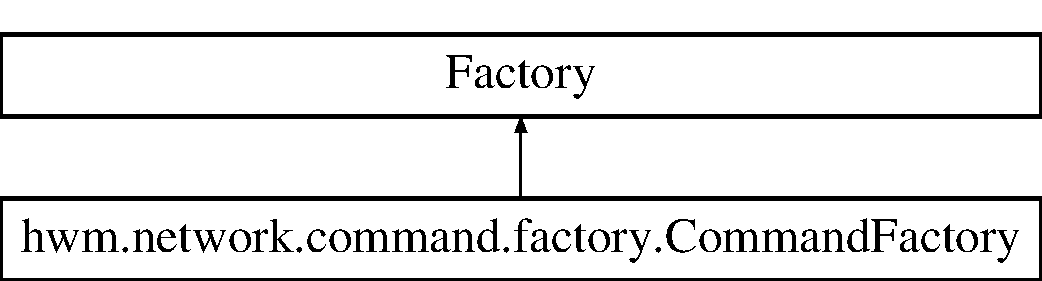
\includegraphics[height=2.000000cm]{classhwm_1_1network_1_1command_1_1factory_1_1_command_factory}
\end{center}
\end{figure}
\subsection*{Public Member Functions}
\begin{DoxyCompactItemize}
\item 
\hypertarget{classhwm_1_1network_1_1command_1_1factory_1_1_command_factory_ab61b598fef0431cc0c5b0c5753e12e82}{def \hyperlink{classhwm_1_1network_1_1command_1_1factory_1_1_command_factory_ab61b598fef0431cc0c5b0c5753e12e82}{\-\_\-\-\_\-init\-\_\-\-\_\-}}\label{classhwm_1_1network_1_1command_1_1factory_1_1_command_factory_ab61b598fef0431cc0c5b0c5753e12e82}

\begin{DoxyCompactList}\small\item\em Sets up the command protocol factory. \end{DoxyCompactList}\item 
def \hyperlink{classhwm_1_1network_1_1command_1_1factory_1_1_command_factory_a16fe7ccd8e21d6fdcc57a34c82f9b2ef}{build\-Protocol}
\begin{DoxyCompactList}\small\item\em Contructs a new command protocol when a connection is made. \end{DoxyCompactList}\end{DoxyCompactItemize}


\subsection{Detailed Description}
Manages command protocol instances as needed. 

This factory is responsible for creating and managing ground station command protocols as users connect and disconnect. 

\subsection{Member Function Documentation}
\hypertarget{classhwm_1_1network_1_1command_1_1factory_1_1_command_factory_a16fe7ccd8e21d6fdcc57a34c82f9b2ef}{\index{hwm\-::network\-::command\-::factory\-::\-Command\-Factory@{hwm\-::network\-::command\-::factory\-::\-Command\-Factory}!build\-Protocol@{build\-Protocol}}
\index{build\-Protocol@{build\-Protocol}!hwm::network::command::factory::CommandFactory@{hwm\-::network\-::command\-::factory\-::\-Command\-Factory}}
\subsubsection[{build\-Protocol}]{\setlength{\rightskip}{0pt plus 5cm}def hwm.\-network.\-command.\-factory.\-Command\-Factory.\-build\-Protocol (
\begin{DoxyParamCaption}
\item[{}]{self, }
\item[{}]{address}
\end{DoxyParamCaption}
)}}\label{classhwm_1_1network_1_1command_1_1factory_1_1_command_factory_a16fe7ccd8e21d6fdcc57a34c82f9b2ef}


Contructs a new command protocol when a connection is made. 


\begin{DoxyParams}{Parameters}
{\em address} & An Address object representing the new connection. \\
\hline
\end{DoxyParams}


The documentation for this class was generated from the following file\-:\begin{DoxyCompactItemize}
\item 
C\-:/\-Users/\-Jimmy/\-Documents/\-Files/\-Work/\-Active Projects/\-M\-X\-L/mercury2/\-Hardware\-\_\-\-Manager/hwm/network/command/factory.\-py\end{DoxyCompactItemize}

\hypertarget{classhwm_1_1core_1_1configuration_1_1_config}{\section{hwm.\-core.\-configuration.\-Config Class Reference}
\label{classhwm_1_1core_1_1configuration_1_1_config}\index{hwm.\-core.\-configuration.\-Config@{hwm.\-core.\-configuration.\-Config}}
}


Provides access to the hardware manager application configuration.  


\subsection*{Public Member Functions}
\begin{DoxyCompactItemize}
\item 
def \hyperlink{classhwm_1_1core_1_1configuration_1_1_config_a06460bf2af249c6601827b2afde8b291}{\-\_\-\-\_\-init\-\_\-\-\_\-}
\begin{DoxyCompactList}\small\item\em Initializes the dictionaries and other member variables used to hold the configuration. \end{DoxyCompactList}\item 
def \hyperlink{classhwm_1_1core_1_1configuration_1_1_config_a805d1df7708afb305e85079d729d8369}{read\-\_\-configuration}
\begin{DoxyCompactList}\small\item\em Loads and parses the specified configuration file. \end{DoxyCompactList}\item 
def \hyperlink{classhwm_1_1core_1_1configuration_1_1_config_ada75769149ea06f7142856fa0a73f5a3}{process\-\_\-configuration}
\begin{DoxyCompactList}\small\item\em Verifies that the required configuration elements have been set. \end{DoxyCompactList}\item 
def \hyperlink{classhwm_1_1core_1_1configuration_1_1_config_ac34da53e95cd38ebc84368e42cbcd95a}{set}
\begin{DoxyCompactList}\small\item\em Sets the indicated configuration option to the provided value. \end{DoxyCompactList}\item 
def \hyperlink{classhwm_1_1core_1_1configuration_1_1_config_a384f394128523c4395e4a6e9f3d5d906}{get}
\begin{DoxyCompactList}\small\item\em Retrieves the specified configuration option. \end{DoxyCompactList}\item 
def \hyperlink{classhwm_1_1core_1_1configuration_1_1_config_a59b1c4c8c34be86e011dd9102e07cfbd}{delete}
\begin{DoxyCompactList}\small\item\em Removes the specified configuration option from the user options dictionary. \end{DoxyCompactList}\end{DoxyCompactItemize}
\subsection*{Public Attributes}
\begin{DoxyCompactItemize}
\item 
\hypertarget{classhwm_1_1core_1_1configuration_1_1_config_a427c9c68035e6d28a05f255593de86aa}{{\bfseries version}}\label{classhwm_1_1core_1_1configuration_1_1_config_a427c9c68035e6d28a05f255593de86aa}

\item 
\hypertarget{classhwm_1_1core_1_1configuration_1_1_config_a0fe0c0b9d227f184980e77d7d0854edc}{{\bfseries verbose\-\_\-startup}}\label{classhwm_1_1core_1_1configuration_1_1_config_a0fe0c0b9d227f184980e77d7d0854edc}

\item 
\hypertarget{classhwm_1_1core_1_1configuration_1_1_config_affca9301b207c467333b9d8b53e63da1}{{\bfseries data\-\_\-directory}}\label{classhwm_1_1core_1_1configuration_1_1_config_affca9301b207c467333b9d8b53e63da1}

\item 
\hypertarget{classhwm_1_1core_1_1configuration_1_1_config_ac08fab7b96bd0ff4f31b3b357b281dda}{{\bfseries options}}\label{classhwm_1_1core_1_1configuration_1_1_config_ac08fab7b96bd0ff4f31b3b357b281dda}

\item 
\hypertarget{classhwm_1_1core_1_1configuration_1_1_config_a76b155d8d10ead2dc5a90fc602a33ffb}{{\bfseries user\-\_\-options}}\label{classhwm_1_1core_1_1configuration_1_1_config_a76b155d8d10ead2dc5a90fc602a33ffb}

\end{DoxyCompactItemize}
\subsection*{Private Member Functions}
\begin{DoxyCompactItemize}
\item 
def \hyperlink{classhwm_1_1core_1_1configuration_1_1_config_af270a1b7fcd55ca884587e9e19411813}{\-\_\-set\-\_\-default\-\_\-configuration}
\begin{DoxyCompactList}\small\item\em Sets the default values for configuration elements that have not been set. \end{DoxyCompactList}\item 
def \hyperlink{classhwm_1_1core_1_1configuration_1_1_config_a95235089ef316715ed60938ebb262fd4}{\-\_\-check\-\_\-required\-\_\-configuration}
\begin{DoxyCompactList}\small\item\em Verifies that the required configuration elements have been set. \end{DoxyCompactList}\end{DoxyCompactItemize}


\subsection{Detailed Description}
Provides access to the hardware manager application configuration. 

This class stores and provides access to the configuration and shared state used by the hardware manager such as the configuration, reservation schedules, and pipeline configuration. In addition, it allows users to store their own configuration options as needed. To use this class import this module (configuration) and assign a local variable to 'Configuration' (makes code easier to test). 

\subsection{Constructor \& Destructor Documentation}
\hypertarget{classhwm_1_1core_1_1configuration_1_1_config_a06460bf2af249c6601827b2afde8b291}{\index{hwm\-::core\-::configuration\-::\-Config@{hwm\-::core\-::configuration\-::\-Config}!\-\_\-\-\_\-init\-\_\-\-\_\-@{\-\_\-\-\_\-init\-\_\-\-\_\-}}
\index{\-\_\-\-\_\-init\-\_\-\-\_\-@{\-\_\-\-\_\-init\-\_\-\-\_\-}!hwm::core::configuration::Config@{hwm\-::core\-::configuration\-::\-Config}}
\subsubsection[{\-\_\-\-\_\-init\-\_\-\-\_\-}]{\setlength{\rightskip}{0pt plus 5cm}def hwm.\-core.\-configuration.\-Config.\-\_\-\-\_\-init\-\_\-\-\_\- (
\begin{DoxyParamCaption}
\item[{}]{self}
\end{DoxyParamCaption}
)}}\label{classhwm_1_1core_1_1configuration_1_1_config_a06460bf2af249c6601827b2afde8b291}


Initializes the dictionaries and other member variables used to hold the configuration. 

\begin{DoxyNote}{Note}
Only user\-\_\-options can be modified during program execution (using the setter/getter). This keeps prevents configuration options from getting altered/deleted. 
\end{DoxyNote}


\subsection{Member Function Documentation}
\hypertarget{classhwm_1_1core_1_1configuration_1_1_config_a95235089ef316715ed60938ebb262fd4}{\index{hwm\-::core\-::configuration\-::\-Config@{hwm\-::core\-::configuration\-::\-Config}!\-\_\-check\-\_\-required\-\_\-configuration@{\-\_\-check\-\_\-required\-\_\-configuration}}
\index{\-\_\-check\-\_\-required\-\_\-configuration@{\-\_\-check\-\_\-required\-\_\-configuration}!hwm::core::configuration::Config@{hwm\-::core\-::configuration\-::\-Config}}
\subsubsection[{\-\_\-check\-\_\-required\-\_\-configuration}]{\setlength{\rightskip}{0pt plus 5cm}def hwm.\-core.\-configuration.\-Config.\-\_\-check\-\_\-required\-\_\-configuration (
\begin{DoxyParamCaption}
\item[{}]{self}
\end{DoxyParamCaption}
)\hspace{0.3cm}{\ttfamily [private]}}}\label{classhwm_1_1core_1_1configuration_1_1_config_a95235089ef316715ed60938ebb262fd4}


Verifies that the required configuration elements have been set. 

\begin{DoxyVerb} This method verifies that the required configuration elements have properly been set.
\end{DoxyVerb}


\begin{DoxyNote}{Note}
If a configuration option is missing, an exception will be thrown detailing the error. This exception will be caught by the global exception handler. 
\end{DoxyNote}
\hypertarget{classhwm_1_1core_1_1configuration_1_1_config_af270a1b7fcd55ca884587e9e19411813}{\index{hwm\-::core\-::configuration\-::\-Config@{hwm\-::core\-::configuration\-::\-Config}!\-\_\-set\-\_\-default\-\_\-configuration@{\-\_\-set\-\_\-default\-\_\-configuration}}
\index{\-\_\-set\-\_\-default\-\_\-configuration@{\-\_\-set\-\_\-default\-\_\-configuration}!hwm::core::configuration::Config@{hwm\-::core\-::configuration\-::\-Config}}
\subsubsection[{\-\_\-set\-\_\-default\-\_\-configuration}]{\setlength{\rightskip}{0pt plus 5cm}def hwm.\-core.\-configuration.\-Config.\-\_\-set\-\_\-default\-\_\-configuration (
\begin{DoxyParamCaption}
\item[{}]{self}
\end{DoxyParamCaption}
)\hspace{0.3cm}{\ttfamily [private]}}}\label{classhwm_1_1core_1_1configuration_1_1_config_af270a1b7fcd55ca884587e9e19411813}


Sets the default values for configuration elements that have not been set. 

\begin{DoxyNote}{Note}
If a configuration option with a default value has been set (most likely from a file by read\-\_\-configuration), that value will be used instead of the default. 
\end{DoxyNote}
\hypertarget{classhwm_1_1core_1_1configuration_1_1_config_a59b1c4c8c34be86e011dd9102e07cfbd}{\index{hwm\-::core\-::configuration\-::\-Config@{hwm\-::core\-::configuration\-::\-Config}!delete@{delete}}
\index{delete@{delete}!hwm::core::configuration::Config@{hwm\-::core\-::configuration\-::\-Config}}
\subsubsection[{delete}]{\setlength{\rightskip}{0pt plus 5cm}def hwm.\-core.\-configuration.\-Config.\-delete (
\begin{DoxyParamCaption}
\item[{}]{self, }
\item[{}]{option\-\_\-key}
\end{DoxyParamCaption}
)}}\label{classhwm_1_1core_1_1configuration_1_1_config_a59b1c4c8c34be86e011dd9102e07cfbd}


Removes the specified configuration option from the user options dictionary. 


\begin{DoxyExceptions}{Exceptions}
{\em \hyperlink{classhwm_1_1core_1_1configuration_1_1_option_protected}{Option\-Protected}} & Thrown if the user tries to delete a protected run-\/time option. \\
\hline
{\em \hyperlink{classhwm_1_1core_1_1configuration_1_1_option_not_found}{Option\-Not\-Found}} & Thrown if the option can't be located.\\
\hline
\end{DoxyExceptions}

\begin{DoxyParams}{Parameters}
{\em option\-\_\-key} & The key of the option to remove. \\
\hline
\end{DoxyParams}
\begin{DoxyReturn}{Returns}
Returns True if the option was successfully deleted. 
\end{DoxyReturn}
\hypertarget{classhwm_1_1core_1_1configuration_1_1_config_a384f394128523c4395e4a6e9f3d5d906}{\index{hwm\-::core\-::configuration\-::\-Config@{hwm\-::core\-::configuration\-::\-Config}!get@{get}}
\index{get@{get}!hwm::core::configuration::Config@{hwm\-::core\-::configuration\-::\-Config}}
\subsubsection[{get}]{\setlength{\rightskip}{0pt plus 5cm}def hwm.\-core.\-configuration.\-Config.\-get (
\begin{DoxyParamCaption}
\item[{}]{self, }
\item[{}]{option\-\_\-key}
\end{DoxyParamCaption}
)}}\label{classhwm_1_1core_1_1configuration_1_1_config_a384f394128523c4395e4a6e9f3d5d906}


Retrieves the specified configuration option. 

\begin{DoxyVerb} This method returns the value of the specified option from either the user defined options or pre-set runtime 
 options.
\end{DoxyVerb}



\begin{DoxyExceptions}{Exceptions}
{\em \hyperlink{classhwm_1_1core_1_1configuration_1_1_option_not_found}{Option\-Not\-Found}} & Thrown if the specified option can't be located in either configuration value dictionary.\\
\hline
\end{DoxyExceptions}

\begin{DoxyParams}{Parameters}
{\em option\-\_\-key} & The key of the option to query for. \\
\hline
\end{DoxyParams}
\begin{DoxyReturn}{Returns}
Returns the value of the specified option if found. 
\end{DoxyReturn}
\hypertarget{classhwm_1_1core_1_1configuration_1_1_config_ada75769149ea06f7142856fa0a73f5a3}{\index{hwm\-::core\-::configuration\-::\-Config@{hwm\-::core\-::configuration\-::\-Config}!process\-\_\-configuration@{process\-\_\-configuration}}
\index{process\-\_\-configuration@{process\-\_\-configuration}!hwm::core::configuration::Config@{hwm\-::core\-::configuration\-::\-Config}}
\subsubsection[{process\-\_\-configuration}]{\setlength{\rightskip}{0pt plus 5cm}def hwm.\-core.\-configuration.\-Config.\-process\-\_\-configuration (
\begin{DoxyParamCaption}
\item[{}]{self}
\end{DoxyParamCaption}
)}}\label{classhwm_1_1core_1_1configuration_1_1_config_ada75769149ea06f7142856fa0a73f5a3}


Verifies that the required configuration elements have been set. 

\begin{DoxyVerb} This method verifies that the required configuration elements have properly been set. These elements were probably
 loaded from a YAML configuration file via read_configuration(). In addition, 
\end{DoxyVerb}


\begin{DoxyNote}{Note}
If a configuration option is missing, an exception will be thrown detailing the error. This exception will be caught by the global exception handler. 

Only configuration options loaded from files before this method is called will be processed. 
\end{DoxyNote}
\hypertarget{classhwm_1_1core_1_1configuration_1_1_config_a805d1df7708afb305e85079d729d8369}{\index{hwm\-::core\-::configuration\-::\-Config@{hwm\-::core\-::configuration\-::\-Config}!read\-\_\-configuration@{read\-\_\-configuration}}
\index{read\-\_\-configuration@{read\-\_\-configuration}!hwm::core::configuration::Config@{hwm\-::core\-::configuration\-::\-Config}}
\subsubsection[{read\-\_\-configuration}]{\setlength{\rightskip}{0pt plus 5cm}def hwm.\-core.\-configuration.\-Config.\-read\-\_\-configuration (
\begin{DoxyParamCaption}
\item[{}]{self, }
\item[{}]{configuration\-\_\-file}
\end{DoxyParamCaption}
)}}\label{classhwm_1_1core_1_1configuration_1_1_config_a805d1df7708afb305e85079d729d8369}


Loads and parses the specified configuration file. 

\begin{DoxyVerb} Reads in all configuration settings from the specified YAML file and stores them in the 'options' dictionary.
\end{DoxyVerb}



\begin{DoxyExceptions}{Exceptions}
{\em I\-O\-Error} & Thrown if the specified file can't be loaded. \\
\hline
{\em Exception} & Thrown if the specified file can't be parsed by the Y\-A\-M\-L parser.\\
\hline
\end{DoxyExceptions}
\begin{DoxyNote}{Note}
All configuration files are in Y\-A\-M\-L format. 

All configurations are assumed to be required (i.\-e. this throws an exception if the file can't be loaded) 

If a file is loaded that contains a previously defined protected option, the previous value will be overridden by the new value. 
\end{DoxyNote}
\begin{DoxySeeAlso}{See Also}
\href{http://en.wikipedia.org/wiki/YAML}{\tt http\-://en.\-wikipedia.\-org/wiki/\-Y\-A\-M\-L}
\end{DoxySeeAlso}

\begin{DoxyParams}{Parameters}
{\em configuration\-\_\-file} & The Y\-A\-M\-L configuration file to load. This is an absolute path. \\
\hline
\end{DoxyParams}
\hypertarget{classhwm_1_1core_1_1configuration_1_1_config_ac34da53e95cd38ebc84368e42cbcd95a}{\index{hwm\-::core\-::configuration\-::\-Config@{hwm\-::core\-::configuration\-::\-Config}!set@{set}}
\index{set@{set}!hwm::core::configuration::Config@{hwm\-::core\-::configuration\-::\-Config}}
\subsubsection[{set}]{\setlength{\rightskip}{0pt plus 5cm}def hwm.\-core.\-configuration.\-Config.\-set (
\begin{DoxyParamCaption}
\item[{}]{self, }
\item[{}]{option\-\_\-key, }
\item[{}]{option\-\_\-value}
\end{DoxyParamCaption}
)}}\label{classhwm_1_1core_1_1configuration_1_1_config_ac34da53e95cd38ebc84368e42cbcd95a}


Sets the indicated configuration option to the provided value. 


\begin{DoxyExceptions}{Exceptions}
{\em \hyperlink{classhwm_1_1core_1_1configuration_1_1_option_protected}{Option\-Protected}} & Thrown if the user tries to modify or set a protected run-\/time key.\\
\hline
\end{DoxyExceptions}

\begin{DoxyParams}{Parameters}
{\em option\-\_\-key} & The key (name) of the option to set. \\
\hline
{\em option\-\_\-value} & The value to assign to the indicated option. \\
\hline
\end{DoxyParams}
\begin{DoxyReturn}{Returns}
Returns True if the option was successfully set. 
\end{DoxyReturn}


The documentation for this class was generated from the following file\-:\begin{DoxyCompactItemize}
\item 
C\-:/\-Users/\-Jimmy/\-Documents/\-Files/\-Work/\-Active Projects/\-M\-X\-L/mercury2/\-Hardware\-\_\-\-Manager/hwm/core/configuration.\-py\end{DoxyCompactItemize}

\hypertarget{classhwm_1_1core_1_1configuration_1_1_option_not_found}{\section{hwm.\-core.\-configuration.\-Option\-Not\-Found Class Reference}
\label{classhwm_1_1core_1_1configuration_1_1_option_not_found}\index{hwm.\-core.\-configuration.\-Option\-Not\-Found@{hwm.\-core.\-configuration.\-Option\-Not\-Found}}
}
Inheritance diagram for hwm.\-core.\-configuration.\-Option\-Not\-Found\-:\begin{figure}[H]
\begin{center}
\leavevmode
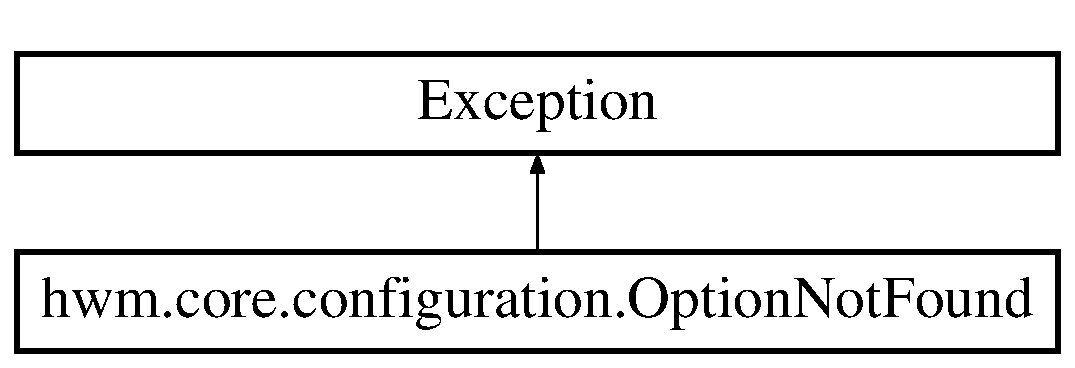
\includegraphics[height=2.000000cm]{classhwm_1_1core_1_1configuration_1_1_option_not_found}
\end{center}
\end{figure}


The documentation for this class was generated from the following file\-:\begin{DoxyCompactItemize}
\item 
hwm/core/configuration.\-py\end{DoxyCompactItemize}

\hypertarget{classhwm_1_1core_1_1configuration_1_1_option_protected}{\section{hwm.\-core.\-configuration.\-Option\-Protected Class Reference}
\label{classhwm_1_1core_1_1configuration_1_1_option_protected}\index{hwm.\-core.\-configuration.\-Option\-Protected@{hwm.\-core.\-configuration.\-Option\-Protected}}
}
Inheritance diagram for hwm.\-core.\-configuration.\-Option\-Protected\-:\begin{figure}[H]
\begin{center}
\leavevmode
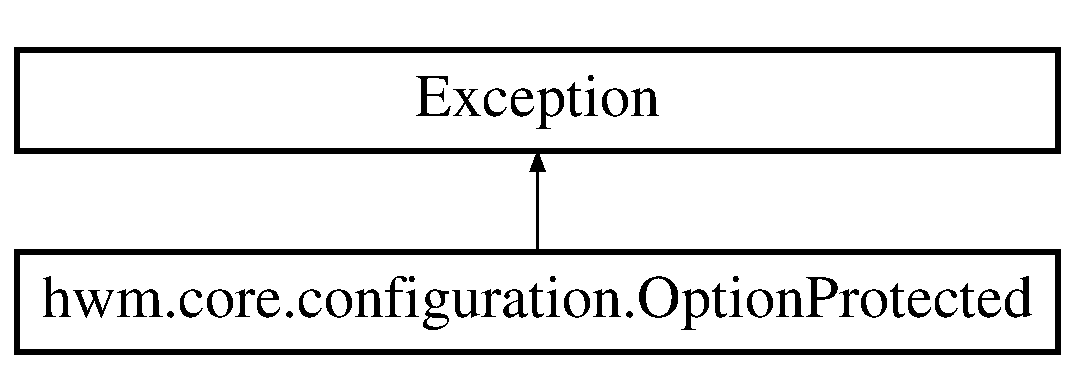
\includegraphics[height=2.000000cm]{classhwm_1_1core_1_1configuration_1_1_option_protected}
\end{center}
\end{figure}


The documentation for this class was generated from the following file\-:\begin{DoxyCompactItemize}
\item 
hwm/core/configuration.\-py\end{DoxyCompactItemize}

\hypertarget{classhwm_1_1hardware_1_1pipelines_1_1pipeline_1_1_pipeline}{\section{hwm.\-hardware.\-pipelines.\-pipeline.\-Pipeline Class Reference}
\label{classhwm_1_1hardware_1_1pipelines_1_1pipeline_1_1_pipeline}\index{hwm.\-hardware.\-pipelines.\-pipeline.\-Pipeline@{hwm.\-hardware.\-pipelines.\-pipeline.\-Pipeline}}
}


Represents and provides access to hardware pipelines.  


\subsection*{Public Member Functions}
\begin{DoxyCompactItemize}
\item 
def \hyperlink{classhwm_1_1hardware_1_1pipelines_1_1pipeline_1_1_pipeline_aed56445fa619c9390ffeba92d924c861}{\-\_\-\-\_\-init\-\_\-\-\_\-}
\begin{DoxyCompactList}\small\item\em Initializes the pipeline with the supplied configuration. \end{DoxyCompactList}\item 
def \hyperlink{classhwm_1_1hardware_1_1pipelines_1_1pipeline_1_1_pipeline_a75e2d36779704a689c0695a3065a69b9}{reserve\-\_\-pipeline}
\begin{DoxyCompactList}\small\item\em Locks the pipeline. \end{DoxyCompactList}\end{DoxyCompactItemize}
\subsection*{Public Attributes}
\begin{DoxyCompactItemize}
\item 
\hypertarget{classhwm_1_1hardware_1_1pipelines_1_1pipeline_1_1_pipeline_a06d0e6687fa8cf71f730ba65704ecc81}{{\bfseries in\-\_\-use}}\label{classhwm_1_1hardware_1_1pipelines_1_1pipeline_1_1_pipeline_a06d0e6687fa8cf71f730ba65704ecc81}

\item 
\hypertarget{classhwm_1_1hardware_1_1pipelines_1_1pipeline_1_1_pipeline_a6a975003dd74bf7c6f201627d61fdc71}{{\bfseries configuration}}\label{classhwm_1_1hardware_1_1pipelines_1_1pipeline_1_1_pipeline_a6a975003dd74bf7c6f201627d61fdc71}

\item 
\hypertarget{classhwm_1_1hardware_1_1pipelines_1_1pipeline_1_1_pipeline_a3227f17d687d49dd432118445e715e29}{{\bfseries id}}\label{classhwm_1_1hardware_1_1pipelines_1_1pipeline_1_1_pipeline_a3227f17d687d49dd432118445e715e29}

\end{DoxyCompactItemize}
\subsection*{Private Member Functions}
\begin{DoxyCompactItemize}
\item 
def \hyperlink{classhwm_1_1hardware_1_1pipelines_1_1pipeline_1_1_pipeline_a89de1b7f4df55a320771c6a4ab928dc2}{\-\_\-validate\-\_\-configuration}
\begin{DoxyCompactList}\small\item\em Validates the pipeline's supplied configuration. \end{DoxyCompactList}\end{DoxyCompactItemize}


\subsection{Detailed Description}
Represents and provides access to hardware pipelines. 

This class represents and provides an interface to the hardware pipelines and associated hardware devices. 

\subsection{Constructor \& Destructor Documentation}
\hypertarget{classhwm_1_1hardware_1_1pipelines_1_1pipeline_1_1_pipeline_aed56445fa619c9390ffeba92d924c861}{\index{hwm\-::hardware\-::pipelines\-::pipeline\-::\-Pipeline@{hwm\-::hardware\-::pipelines\-::pipeline\-::\-Pipeline}!\-\_\-\-\_\-init\-\_\-\-\_\-@{\-\_\-\-\_\-init\-\_\-\-\_\-}}
\index{\-\_\-\-\_\-init\-\_\-\-\_\-@{\-\_\-\-\_\-init\-\_\-\-\_\-}!hwm::hardware::pipelines::pipeline::Pipeline@{hwm\-::hardware\-::pipelines\-::pipeline\-::\-Pipeline}}
\subsubsection[{\-\_\-\-\_\-init\-\_\-\-\_\-}]{\setlength{\rightskip}{0pt plus 5cm}def hwm.\-hardware.\-pipelines.\-pipeline.\-Pipeline.\-\_\-\-\_\-init\-\_\-\-\_\- (
\begin{DoxyParamCaption}
\item[{}]{self, }
\item[{}]{pipeline\-\_\-configuration}
\end{DoxyParamCaption}
)}}\label{classhwm_1_1hardware_1_1pipelines_1_1pipeline_1_1_pipeline_aed56445fa619c9390ffeba92d924c861}


Initializes the pipeline with the supplied configuration. 

\begin{DoxyNote}{Note}
The pipelines are initialized by the pipeline manager, not individually. 

This method may pass on exceptions from the pipeline configuration validator.
\end{DoxyNote}

\begin{DoxyParams}{Parameters}
{\em pipeline\-\_\-configuration} & A dictionary containing the settings to initialize the pipeline with. This is supplied by the pipeline manager and is loaded from the pipeline configuration file. \\
\hline
\end{DoxyParams}


\subsection{Member Function Documentation}
\hypertarget{classhwm_1_1hardware_1_1pipelines_1_1pipeline_1_1_pipeline_a89de1b7f4df55a320771c6a4ab928dc2}{\index{hwm\-::hardware\-::pipelines\-::pipeline\-::\-Pipeline@{hwm\-::hardware\-::pipelines\-::pipeline\-::\-Pipeline}!\-\_\-validate\-\_\-configuration@{\-\_\-validate\-\_\-configuration}}
\index{\-\_\-validate\-\_\-configuration@{\-\_\-validate\-\_\-configuration}!hwm::hardware::pipelines::pipeline::Pipeline@{hwm\-::hardware\-::pipelines\-::pipeline\-::\-Pipeline}}
\subsubsection[{\-\_\-validate\-\_\-configuration}]{\setlength{\rightskip}{0pt plus 5cm}def hwm.\-hardware.\-pipelines.\-pipeline.\-Pipeline.\-\_\-validate\-\_\-configuration (
\begin{DoxyParamCaption}
\item[{}]{self}
\end{DoxyParamCaption}
)\hspace{0.3cm}{\ttfamily [private]}}}\label{classhwm_1_1hardware_1_1pipelines_1_1pipeline_1_1_pipeline_a89de1b7f4df55a320771c6a4ab928dc2}


Validates the pipeline's supplied configuration. 

\begin{DoxyVerb} This method validates the pipeline's supplied configuration against the requirements.
\end{DoxyVerb}



\begin{DoxyExceptions}{Exceptions}
{\em Throws} & \hyperlink{classhwm_1_1hardware_1_1pipelines_1_1pipeline_1_1_pipeline_invalid_configuration}{Pipeline\-Invalid\-Configuration} is the supplied configuration is invalid. \\
\hline
\end{DoxyExceptions}
\hypertarget{classhwm_1_1hardware_1_1pipelines_1_1pipeline_1_1_pipeline_a75e2d36779704a689c0695a3065a69b9}{\index{hwm\-::hardware\-::pipelines\-::pipeline\-::\-Pipeline@{hwm\-::hardware\-::pipelines\-::pipeline\-::\-Pipeline}!reserve\-\_\-pipeline@{reserve\-\_\-pipeline}}
\index{reserve\-\_\-pipeline@{reserve\-\_\-pipeline}!hwm::hardware::pipelines::pipeline::Pipeline@{hwm\-::hardware\-::pipelines\-::pipeline\-::\-Pipeline}}
\subsubsection[{reserve\-\_\-pipeline}]{\setlength{\rightskip}{0pt plus 5cm}def hwm.\-hardware.\-pipelines.\-pipeline.\-Pipeline.\-reserve\-\_\-pipeline (
\begin{DoxyParamCaption}
\item[{}]{self}
\end{DoxyParamCaption}
)}}\label{classhwm_1_1hardware_1_1pipelines_1_1pipeline_1_1_pipeline_a75e2d36779704a689c0695a3065a69b9}


Locks the pipeline. 

When called, this method checks if the pipeline is currently being used. If it is, an exception is generated. If it isn't then the pipeline is locked. 

The documentation for this class was generated from the following file\-:\begin{DoxyCompactItemize}
\item 
C\-:/\-Users/\-Jimmy/\-Documents/\-Files/\-Work/\-Active Projects/\-M\-X\-L/mercury2/\-Hardware\-\_\-\-Manager/hwm/hardware/pipelines/pipeline.\-py\end{DoxyCompactItemize}

\hypertarget{classhwm_1_1hardware_1_1pipelines_1_1pipeline_1_1_pipeline_in_use}{\section{hwm.\-hardware.\-pipelines.\-pipeline.\-Pipeline\-In\-Use Class Reference}
\label{classhwm_1_1hardware_1_1pipelines_1_1pipeline_1_1_pipeline_in_use}\index{hwm.\-hardware.\-pipelines.\-pipeline.\-Pipeline\-In\-Use@{hwm.\-hardware.\-pipelines.\-pipeline.\-Pipeline\-In\-Use}}
}
Inheritance diagram for hwm.\-hardware.\-pipelines.\-pipeline.\-Pipeline\-In\-Use\-:\begin{figure}[H]
\begin{center}
\leavevmode
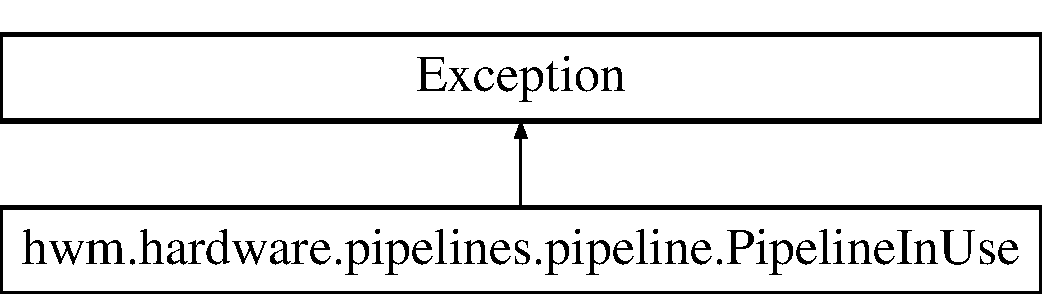
\includegraphics[height=3.000000cm]{classhwm_1_1hardware_1_1pipelines_1_1pipeline_1_1_pipeline_in_use}
\end{center}
\end{figure}


The documentation for this class was generated from the following file\-:\begin{DoxyCompactItemize}
\item 
hwm/hardware/pipelines/pipeline.\-py\end{DoxyCompactItemize}

\hypertarget{classhwm_1_1hardware_1_1pipelines_1_1pipeline_1_1_pipeline_invalid_configuration}{\section{hwm.\-hardware.\-pipelines.\-pipeline.\-Pipeline\-Invalid\-Configuration Class Reference}
\label{classhwm_1_1hardware_1_1pipelines_1_1pipeline_1_1_pipeline_invalid_configuration}\index{hwm.\-hardware.\-pipelines.\-pipeline.\-Pipeline\-Invalid\-Configuration@{hwm.\-hardware.\-pipelines.\-pipeline.\-Pipeline\-Invalid\-Configuration}}
}
Inheritance diagram for hwm.\-hardware.\-pipelines.\-pipeline.\-Pipeline\-Invalid\-Configuration\-:\begin{figure}[H]
\begin{center}
\leavevmode
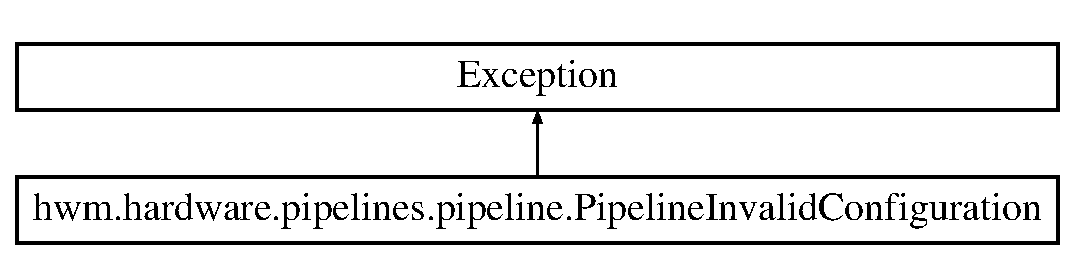
\includegraphics[height=2.000000cm]{classhwm_1_1hardware_1_1pipelines_1_1pipeline_1_1_pipeline_invalid_configuration}
\end{center}
\end{figure}


The documentation for this class was generated from the following file\-:\begin{DoxyCompactItemize}
\item 
C\-:/\-Users/\-Jimmy/\-Documents/\-Files/\-Work/\-Active Projects/\-M\-X\-L/mercury2/\-Hardware\-\_\-\-Manager/hwm/hardware/pipelines/pipeline.\-py\end{DoxyCompactItemize}

\hypertarget{classhwm_1_1hardware_1_1pipelines_1_1manager_1_1_pipeline_manager}{\section{hwm.\-hardware.\-pipelines.\-manager.\-Pipeline\-Manager Class Reference}
\label{classhwm_1_1hardware_1_1pipelines_1_1manager_1_1_pipeline_manager}\index{hwm.\-hardware.\-pipelines.\-manager.\-Pipeline\-Manager@{hwm.\-hardware.\-pipelines.\-manager.\-Pipeline\-Manager}}
}


Provides access the collection of available hardware pipelines.  


\subsection*{Public Member Functions}
\begin{DoxyCompactItemize}
\item 
def \hyperlink{classhwm_1_1hardware_1_1pipelines_1_1manager_1_1_pipeline_manager_a88a42b5d8f14bb37d5618cd29452126d}{\-\_\-\-\_\-init\-\_\-\-\_\-}
\begin{DoxyCompactList}\small\item\em Sets up the pipeline manager. \end{DoxyCompactList}\item 
def \hyperlink{classhwm_1_1hardware_1_1pipelines_1_1manager_1_1_pipeline_manager_acd2d1d93204110d7256c8cbb34cde804}{get\-\_\-pipeline}
\begin{DoxyCompactList}\small\item\em Returns a reference to the specified pipeline. \end{DoxyCompactList}\end{DoxyCompactItemize}
\subsection*{Public Attributes}
\begin{DoxyCompactItemize}
\item 
\hypertarget{classhwm_1_1hardware_1_1pipelines_1_1manager_1_1_pipeline_manager_a11e66d6149717d994105088073f3233b}{{\bfseries config}}\label{classhwm_1_1hardware_1_1pipelines_1_1manager_1_1_pipeline_manager_a11e66d6149717d994105088073f3233b}

\item 
\hypertarget{classhwm_1_1hardware_1_1pipelines_1_1manager_1_1_pipeline_manager_a8aa2912c371eb0cc95d127b15b8164aa}{{\bfseries device\-\_\-manager}}\label{classhwm_1_1hardware_1_1pipelines_1_1manager_1_1_pipeline_manager_a8aa2912c371eb0cc95d127b15b8164aa}

\item 
\hypertarget{classhwm_1_1hardware_1_1pipelines_1_1manager_1_1_pipeline_manager_a108ced2236088b116828b55fb7a0d98d}{{\bfseries command\-\_\-parser}}\label{classhwm_1_1hardware_1_1pipelines_1_1manager_1_1_pipeline_manager_a108ced2236088b116828b55fb7a0d98d}

\item 
\hypertarget{classhwm_1_1hardware_1_1pipelines_1_1manager_1_1_pipeline_manager_a3984be455a8589fa8cc5ec28cb2ffb80}{{\bfseries pipelines}}\label{classhwm_1_1hardware_1_1pipelines_1_1manager_1_1_pipeline_manager_a3984be455a8589fa8cc5ec28cb2ffb80}

\end{DoxyCompactItemize}
\subsection*{Private Member Functions}
\begin{DoxyCompactItemize}
\item 
def \hyperlink{classhwm_1_1hardware_1_1pipelines_1_1manager_1_1_pipeline_manager_a19b0c2d59d9b7168523647ef3dffe5ad}{\-\_\-initialize\-\_\-pipelines}
\begin{DoxyCompactList}\small\item\em Initializes the configured pipelines. \end{DoxyCompactList}\item 
def \hyperlink{classhwm_1_1hardware_1_1pipelines_1_1manager_1_1_pipeline_manager_a30049fcecdad73fd9dcb18c216506fc7}{\-\_\-validate\-\_\-pipeline\-\_\-schema}
\begin{DoxyCompactList}\small\item\em Validates the provided pipeline configuration. \end{DoxyCompactList}\end{DoxyCompactItemize}


\subsection{Detailed Description}
Provides access the collection of available hardware pipelines. 

This class initializes and manages the collection of loaded hardware pipelines. 

\subsection{Constructor \& Destructor Documentation}
\hypertarget{classhwm_1_1hardware_1_1pipelines_1_1manager_1_1_pipeline_manager_a88a42b5d8f14bb37d5618cd29452126d}{\index{hwm\-::hardware\-::pipelines\-::manager\-::\-Pipeline\-Manager@{hwm\-::hardware\-::pipelines\-::manager\-::\-Pipeline\-Manager}!\-\_\-\-\_\-init\-\_\-\-\_\-@{\-\_\-\-\_\-init\-\_\-\-\_\-}}
\index{\-\_\-\-\_\-init\-\_\-\-\_\-@{\-\_\-\-\_\-init\-\_\-\-\_\-}!hwm::hardware::pipelines::manager::PipelineManager@{hwm\-::hardware\-::pipelines\-::manager\-::\-Pipeline\-Manager}}
\subsubsection[{\-\_\-\-\_\-init\-\_\-\-\_\-}]{\setlength{\rightskip}{0pt plus 5cm}def hwm.\-hardware.\-pipelines.\-manager.\-Pipeline\-Manager.\-\_\-\-\_\-init\-\_\-\-\_\- (
\begin{DoxyParamCaption}
\item[{}]{self, }
\item[{}]{device\-\_\-manager, }
\item[{}]{command\-\_\-parser}
\end{DoxyParamCaption}
)}}\label{classhwm_1_1hardware_1_1pipelines_1_1manager_1_1_pipeline_manager_a88a42b5d8f14bb37d5618cd29452126d}


Sets up the pipeline manager. 

\begin{DoxyVerb} This constructor sets up the pipeline manager and calls a method that initializes the available pipelines.
\end{DoxyVerb}


\begin{DoxyNote}{Note}
This class does not load the pipeline configuration file itself. Instead, Configuration is instructed to load it at runtime and this class accesses it via the 'configuration' module. If this class is initialized before the pipeline configuration has been loaded an exception will be raised
\end{DoxyNote}

\begin{DoxyExceptions}{Exceptions}
{\em May} & pass on exceptions from the pipeline initialization process (see \-\_\-initialize\-\_\-pipelines).\\
\hline
\end{DoxyExceptions}

\begin{DoxyParams}{Parameters}
{\em device\-\_\-manager} & A reference to the Device\-Manager instance that should be used. \\
\hline
{\em command\-\_\-parser} & A reference to a Command\-Parser that will be used to process pipeline setup commands. \\
\hline
\end{DoxyParams}


\subsection{Member Function Documentation}
\hypertarget{classhwm_1_1hardware_1_1pipelines_1_1manager_1_1_pipeline_manager_a19b0c2d59d9b7168523647ef3dffe5ad}{\index{hwm\-::hardware\-::pipelines\-::manager\-::\-Pipeline\-Manager@{hwm\-::hardware\-::pipelines\-::manager\-::\-Pipeline\-Manager}!\-\_\-initialize\-\_\-pipelines@{\-\_\-initialize\-\_\-pipelines}}
\index{\-\_\-initialize\-\_\-pipelines@{\-\_\-initialize\-\_\-pipelines}!hwm::hardware::pipelines::manager::PipelineManager@{hwm\-::hardware\-::pipelines\-::manager\-::\-Pipeline\-Manager}}
\subsubsection[{\-\_\-initialize\-\_\-pipelines}]{\setlength{\rightskip}{0pt plus 5cm}def hwm.\-hardware.\-pipelines.\-manager.\-Pipeline\-Manager.\-\_\-initialize\-\_\-pipelines (
\begin{DoxyParamCaption}
\item[{}]{self}
\end{DoxyParamCaption}
)\hspace{0.3cm}{\ttfamily [private]}}}\label{classhwm_1_1hardware_1_1pipelines_1_1manager_1_1_pipeline_manager_a19b0c2d59d9b7168523647ef3dffe5ad}


Initializes the configured pipelines. 

\begin{DoxyVerb} This method initializes all of the configured pipelines (i.e. available in the configuration) and saves their
 references.
\end{DoxyVerb}



\begin{DoxyExceptions}{Exceptions}
{\em Throws} & Pipelines\-All\-Ready\-Initialized if this method is called after pipelines have been initialized. \\
\hline
{\em Throws} & \hyperlink{classhwm_1_1hardware_1_1pipelines_1_1manager_1_1_pipelines_not_defined}{Pipelines\-Not\-Defined} if no pipelines are defined in the runtime configuration. \\
\hline
{\em May} & pass on \hyperlink{classhwm_1_1hardware_1_1pipelines_1_1manager_1_1_pipeline_schema_invalid}{Pipeline\-Schema\-Invalid} exceptions if the pipeline configuration doesn't match the defined schema. \\
\hline
{\em May} & pass on Pipeline\-Config\-Invalid exceptions if the pipeline configuration contains other errors. \\
\hline
\end{DoxyExceptions}
\hypertarget{classhwm_1_1hardware_1_1pipelines_1_1manager_1_1_pipeline_manager_a30049fcecdad73fd9dcb18c216506fc7}{\index{hwm\-::hardware\-::pipelines\-::manager\-::\-Pipeline\-Manager@{hwm\-::hardware\-::pipelines\-::manager\-::\-Pipeline\-Manager}!\-\_\-validate\-\_\-pipeline\-\_\-schema@{\-\_\-validate\-\_\-pipeline\-\_\-schema}}
\index{\-\_\-validate\-\_\-pipeline\-\_\-schema@{\-\_\-validate\-\_\-pipeline\-\_\-schema}!hwm::hardware::pipelines::manager::PipelineManager@{hwm\-::hardware\-::pipelines\-::manager\-::\-Pipeline\-Manager}}
\subsubsection[{\-\_\-validate\-\_\-pipeline\-\_\-schema}]{\setlength{\rightskip}{0pt plus 5cm}def hwm.\-hardware.\-pipelines.\-manager.\-Pipeline\-Manager.\-\_\-validate\-\_\-pipeline\-\_\-schema (
\begin{DoxyParamCaption}
\item[{}]{self, }
\item[{}]{pipeline\-\_\-configuration}
\end{DoxyParamCaption}
)\hspace{0.3cm}{\ttfamily [private]}}}\label{classhwm_1_1hardware_1_1pipelines_1_1manager_1_1_pipeline_manager_a30049fcecdad73fd9dcb18c216506fc7}


Validates the provided pipeline configuration. 

\begin{DoxyVerb} This method validates the provided pipeline configuration (loaded from the configuration files) by comparing it
 against the defined schema.
\end{DoxyVerb}


\begin{DoxyNote}{Note}
Each pipeline class may perform additional validations when initialized. This method simply checks the pipeline configuration schema as a whole.
\end{DoxyNote}

\begin{DoxyExceptions}{Exceptions}
{\em Throws} & \hyperlink{classhwm_1_1hardware_1_1pipelines_1_1manager_1_1_pipeline_schema_invalid}{Pipeline\-Schema\-Invalid} if the provided pipeline configuration schema is invalid.\\
\hline
\end{DoxyExceptions}

\begin{DoxyParams}{Parameters}
{\em pipeline\-\_\-configuration} & An object containing the pipeline configuration from the Y\-A\-M\-L configuration files. \\
\hline
\end{DoxyParams}
\hypertarget{classhwm_1_1hardware_1_1pipelines_1_1manager_1_1_pipeline_manager_acd2d1d93204110d7256c8cbb34cde804}{\index{hwm\-::hardware\-::pipelines\-::manager\-::\-Pipeline\-Manager@{hwm\-::hardware\-::pipelines\-::manager\-::\-Pipeline\-Manager}!get\-\_\-pipeline@{get\-\_\-pipeline}}
\index{get\-\_\-pipeline@{get\-\_\-pipeline}!hwm::hardware::pipelines::manager::PipelineManager@{hwm\-::hardware\-::pipelines\-::manager\-::\-Pipeline\-Manager}}
\subsubsection[{get\-\_\-pipeline}]{\setlength{\rightskip}{0pt plus 5cm}def hwm.\-hardware.\-pipelines.\-manager.\-Pipeline\-Manager.\-get\-\_\-pipeline (
\begin{DoxyParamCaption}
\item[{}]{self, }
\item[{}]{pipeline\-\_\-id}
\end{DoxyParamCaption}
)}}\label{classhwm_1_1hardware_1_1pipelines_1_1manager_1_1_pipeline_manager_acd2d1d93204110d7256c8cbb34cde804}


Returns a reference to the specified pipeline. 

\begin{DoxyNote}{Note}
This method does not perform any pipeline locking. That is managed by the individual pipeline classes and is typically triggered by the session coordinator.
\end{DoxyNote}

\begin{DoxyExceptions}{Exceptions}
{\em Throws} & \hyperlink{classhwm_1_1hardware_1_1pipelines_1_1manager_1_1_pipeline_not_found}{Pipeline\-Not\-Found} when the requested pipeline can't be found.\\
\hline
\end{DoxyExceptions}

\begin{DoxyParams}{Parameters}
{\em pipeline\-\_\-id} & The I\-D of the requested pipeline. \\
\hline
\end{DoxyParams}
\begin{DoxyReturn}{Returns}
Returns a reference to the specified pipeline object. 
\end{DoxyReturn}


The documentation for this class was generated from the following file\-:\begin{DoxyCompactItemize}
\item 
hwm/hardware/pipelines/manager.\-py\end{DoxyCompactItemize}

\hypertarget{classhwm_1_1hardware_1_1pipelines_1_1manager_1_1_pipeline_not_found}{\section{hwm.\-hardware.\-pipelines.\-manager.\-Pipeline\-Not\-Found Class Reference}
\label{classhwm_1_1hardware_1_1pipelines_1_1manager_1_1_pipeline_not_found}\index{hwm.\-hardware.\-pipelines.\-manager.\-Pipeline\-Not\-Found@{hwm.\-hardware.\-pipelines.\-manager.\-Pipeline\-Not\-Found}}
}
Inheritance diagram for hwm.\-hardware.\-pipelines.\-manager.\-Pipeline\-Not\-Found\-:\begin{figure}[H]
\begin{center}
\leavevmode
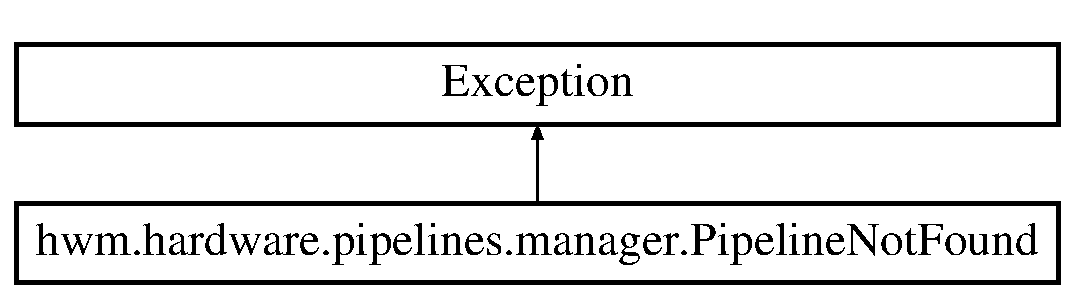
\includegraphics[height=3.000000cm]{classhwm_1_1hardware_1_1pipelines_1_1manager_1_1_pipeline_not_found}
\end{center}
\end{figure}


The documentation for this class was generated from the following file\-:\begin{DoxyCompactItemize}
\item 
hwm/hardware/pipelines/manager.\-py\end{DoxyCompactItemize}

\hypertarget{classhwm_1_1hardware_1_1pipelines_1_1manager_1_1_pipelines_all_ready_initialized}{\section{hwm.\-hardware.\-pipelines.\-manager.\-Pipelines\-All\-Ready\-Initialized Class Reference}
\label{classhwm_1_1hardware_1_1pipelines_1_1manager_1_1_pipelines_all_ready_initialized}\index{hwm.\-hardware.\-pipelines.\-manager.\-Pipelines\-All\-Ready\-Initialized@{hwm.\-hardware.\-pipelines.\-manager.\-Pipelines\-All\-Ready\-Initialized}}
}
Inheritance diagram for hwm.\-hardware.\-pipelines.\-manager.\-Pipelines\-All\-Ready\-Initialized\-:\begin{figure}[H]
\begin{center}
\leavevmode
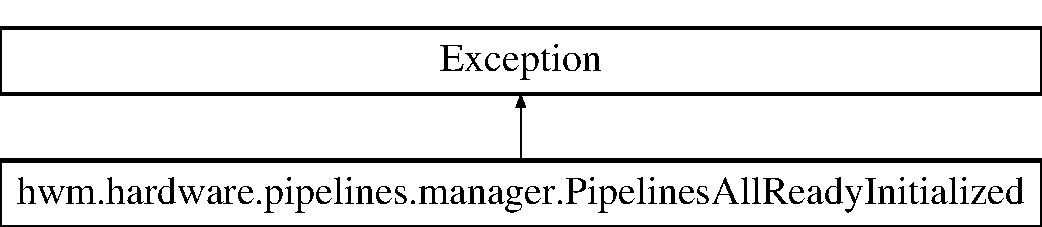
\includegraphics[height=2.000000cm]{classhwm_1_1hardware_1_1pipelines_1_1manager_1_1_pipelines_all_ready_initialized}
\end{center}
\end{figure}


The documentation for this class was generated from the following file\-:\begin{DoxyCompactItemize}
\item 
C\-:/\-Users/\-Jimmy/\-Documents/\-Files/\-Work/\-Active Projects/\-M\-X\-L/mercury2/\-Hardware\-\_\-\-Manager/hwm/hardware/pipelines/manager.\-py\end{DoxyCompactItemize}

\hypertarget{classhwm_1_1hardware_1_1pipelines_1_1manager_1_1_pipelines_not_defined}{\section{hwm.\-hardware.\-pipelines.\-manager.\-Pipelines\-Not\-Defined Class Reference}
\label{classhwm_1_1hardware_1_1pipelines_1_1manager_1_1_pipelines_not_defined}\index{hwm.\-hardware.\-pipelines.\-manager.\-Pipelines\-Not\-Defined@{hwm.\-hardware.\-pipelines.\-manager.\-Pipelines\-Not\-Defined}}
}
Inheritance diagram for hwm.\-hardware.\-pipelines.\-manager.\-Pipelines\-Not\-Defined\-:\begin{figure}[H]
\begin{center}
\leavevmode
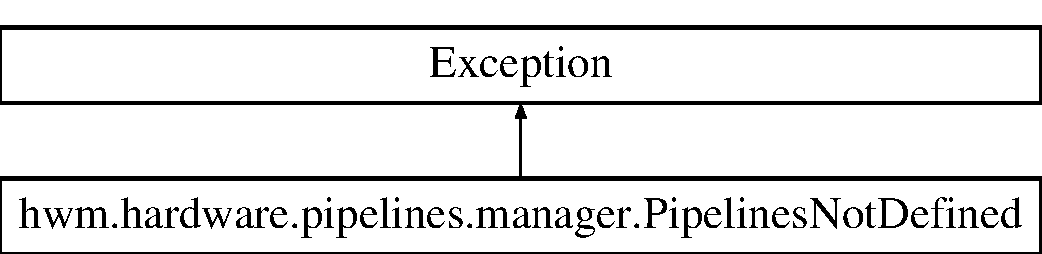
\includegraphics[height=3.000000cm]{classhwm_1_1hardware_1_1pipelines_1_1manager_1_1_pipelines_not_defined}
\end{center}
\end{figure}


The documentation for this class was generated from the following file\-:\begin{DoxyCompactItemize}
\item 
hwm/hardware/pipelines/manager.\-py\end{DoxyCompactItemize}

\hypertarget{classhwm_1_1sessions_1_1schedule_1_1_schedule_error}{\section{hwm.\-sessions.\-schedule.\-Schedule\-Error Class Reference}
\label{classhwm_1_1sessions_1_1schedule_1_1_schedule_error}\index{hwm.\-sessions.\-schedule.\-Schedule\-Error@{hwm.\-sessions.\-schedule.\-Schedule\-Error}}
}
Inheritance diagram for hwm.\-sessions.\-schedule.\-Schedule\-Error\-:\begin{figure}[H]
\begin{center}
\leavevmode
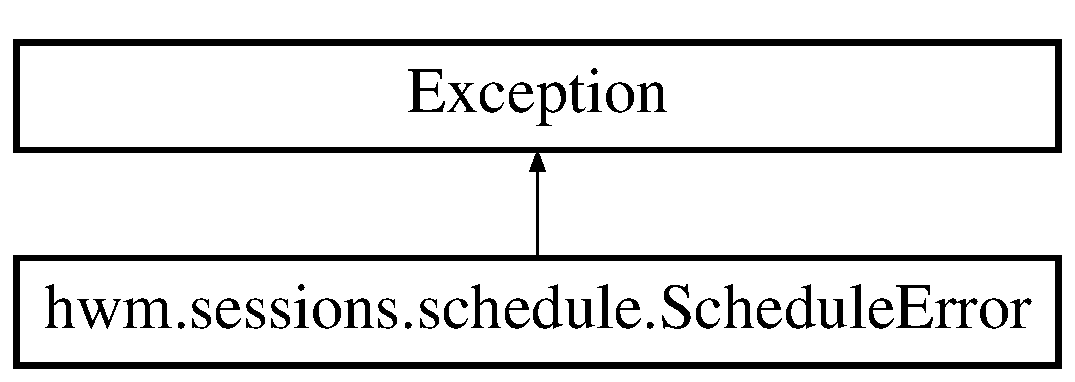
\includegraphics[height=2.000000cm]{classhwm_1_1sessions_1_1schedule_1_1_schedule_error}
\end{center}
\end{figure}


The documentation for this class was generated from the following file\-:\begin{DoxyCompactItemize}
\item 
hwm/sessions/schedule.\-py\end{DoxyCompactItemize}

\hypertarget{classhwm_1_1sessions_1_1schedule_1_1_schedule_manager}{\section{hwm.\-sessions.\-schedule.\-Schedule\-Manager Class Reference}
\label{classhwm_1_1sessions_1_1schedule_1_1_schedule_manager}\index{hwm.\-sessions.\-schedule.\-Schedule\-Manager@{hwm.\-sessions.\-schedule.\-Schedule\-Manager}}
}


Represents a reservation access schedule.  


\subsection*{Public Member Functions}
\begin{DoxyCompactItemize}
\item 
def \hyperlink{classhwm_1_1sessions_1_1schedule_1_1_schedule_manager_a0143ac24564e0a7176921772f522acf4}{\-\_\-\-\_\-init\-\_\-\-\_\-}
\begin{DoxyCompactList}\small\item\em Initializes the schedule instance. \end{DoxyCompactList}\item 
def \hyperlink{classhwm_1_1sessions_1_1schedule_1_1_schedule_manager_a796d64f28ba7cf37b1958077aba60a09}{update\-\_\-schedule}
\begin{DoxyCompactList}\small\item\em Downloads the most recent version of the schedule from the active source. \end{DoxyCompactList}\item 
def \hyperlink{classhwm_1_1sessions_1_1schedule_1_1_schedule_manager_a8d1904cfc12d70c97ac0ad66d02b57b4}{get\-\_\-active\-\_\-reservations}
\begin{DoxyCompactList}\small\item\em Returns a list of the currently active reservations (by timestamp). \end{DoxyCompactList}\end{DoxyCompactItemize}
\subsection*{Public Attributes}
\begin{DoxyCompactItemize}
\item 
\hypertarget{classhwm_1_1sessions_1_1schedule_1_1_schedule_manager_afa995b0beb3c784fdb000e3e831b282e}{{\bfseries config}}\label{classhwm_1_1sessions_1_1schedule_1_1_schedule_manager_afa995b0beb3c784fdb000e3e831b282e}

\item 
\hypertarget{classhwm_1_1sessions_1_1schedule_1_1_schedule_manager_a7d2a931d793fc0a6db2e18ab877b7c75}{{\bfseries use\-\_\-network\-\_\-schedule}}\label{classhwm_1_1sessions_1_1schedule_1_1_schedule_manager_a7d2a931d793fc0a6db2e18ab877b7c75}

\item 
\hypertarget{classhwm_1_1sessions_1_1schedule_1_1_schedule_manager_a80b5a9421afb5f761dfbf5694d168b89}{{\bfseries schedule\-\_\-location}}\label{classhwm_1_1sessions_1_1schedule_1_1_schedule_manager_a80b5a9421afb5f761dfbf5694d168b89}

\item 
\hypertarget{classhwm_1_1sessions_1_1schedule_1_1_schedule_manager_a32b0341fa62d60fe41040ebcaaf2bf0a}{{\bfseries schedule}}\label{classhwm_1_1sessions_1_1schedule_1_1_schedule_manager_a32b0341fa62d60fe41040ebcaaf2bf0a}

\item 
\hypertarget{classhwm_1_1sessions_1_1schedule_1_1_schedule_manager_a9327b4c4367245911c7ff3bc2ffd81f6}{{\bfseries last\-\_\-updated}}\label{classhwm_1_1sessions_1_1schedule_1_1_schedule_manager_a9327b4c4367245911c7ff3bc2ffd81f6}

\end{DoxyCompactItemize}
\subsection*{Private Member Functions}
\begin{DoxyCompactItemize}
\item 
def \hyperlink{classhwm_1_1sessions_1_1schedule_1_1_schedule_manager_a022e98a41d6254ab8be51509089c11e2}{\-\_\-validate\-\_\-schedule}
\begin{DoxyCompactList}\small\item\em Validates the newly loaded schedule J\-S\-O\-N. \end{DoxyCompactList}\item 
def \hyperlink{classhwm_1_1sessions_1_1schedule_1_1_schedule_manager_a969595d4ed4ef73bf5709a4910afb548}{\-\_\-save\-\_\-schedule}
\begin{DoxyCompactList}\small\item\em Saves the provided schedule to the \hyperlink{classhwm_1_1sessions_1_1schedule_1_1_schedule_manager}{Schedule\-Manager} class instance. \end{DoxyCompactList}\item 
def \hyperlink{classhwm_1_1sessions_1_1schedule_1_1_schedule_manager_a4eb795805cbf4dd66c7c4774f9c07ea9}{\-\_\-download\-\_\-remote\-\_\-schedule}
\begin{DoxyCompactList}\small\item\em Loads the schedule from the schedule's U\-R\-L. \end{DoxyCompactList}\item 
def \hyperlink{classhwm_1_1sessions_1_1schedule_1_1_schedule_manager_ab40776c55c8d1f12a0d59f55bc716675}{\-\_\-download\-\_\-local\-\_\-schedule}
\begin{DoxyCompactList}\small\item\em Loads the schedule from the local disk. \end{DoxyCompactList}\end{DoxyCompactItemize}


\subsection{Detailed Description}
Represents a reservation access schedule. 

This class provides access to a copy of the reservation schedule. That hardware manager can use \hyperlink{classhwm_1_1sessions_1_1schedule_1_1_schedule_manager}{Schedule\-Manager} to\-:
\begin{DoxyItemize}
\item Download new copies of the reservation schedule from the user interface
\item Query for specific reservations
\item Access newly active reservations 
\end{DoxyItemize}

\subsection{Constructor \& Destructor Documentation}
\hypertarget{classhwm_1_1sessions_1_1schedule_1_1_schedule_manager_a0143ac24564e0a7176921772f522acf4}{\index{hwm\-::sessions\-::schedule\-::\-Schedule\-Manager@{hwm\-::sessions\-::schedule\-::\-Schedule\-Manager}!\-\_\-\-\_\-init\-\_\-\-\_\-@{\-\_\-\-\_\-init\-\_\-\-\_\-}}
\index{\-\_\-\-\_\-init\-\_\-\-\_\-@{\-\_\-\-\_\-init\-\_\-\-\_\-}!hwm::sessions::schedule::ScheduleManager@{hwm\-::sessions\-::schedule\-::\-Schedule\-Manager}}
\subsubsection[{\-\_\-\-\_\-init\-\_\-\-\_\-}]{\setlength{\rightskip}{0pt plus 5cm}def hwm.\-sessions.\-schedule.\-Schedule\-Manager.\-\_\-\-\_\-init\-\_\-\-\_\- (
\begin{DoxyParamCaption}
\item[{}]{self, }
\item[{}]{schedule\-\_\-endpoint}
\end{DoxyParamCaption}
)}}\label{classhwm_1_1sessions_1_1schedule_1_1_schedule_manager_a0143ac24564e0a7176921772f522acf4}


Initializes the schedule instance. 


\begin{DoxyParams}{Parameters}
{\em schedule\-\_\-endpoint} & Where to load the reservation schedule from. This can either be a local file or a network address (such as the mercury2 user interface A\-P\-I). If it begins with 'http', it will be treated as a network address. \\
\hline
\end{DoxyParams}


\subsection{Member Function Documentation}
\hypertarget{classhwm_1_1sessions_1_1schedule_1_1_schedule_manager_ab40776c55c8d1f12a0d59f55bc716675}{\index{hwm\-::sessions\-::schedule\-::\-Schedule\-Manager@{hwm\-::sessions\-::schedule\-::\-Schedule\-Manager}!\-\_\-download\-\_\-local\-\_\-schedule@{\-\_\-download\-\_\-local\-\_\-schedule}}
\index{\-\_\-download\-\_\-local\-\_\-schedule@{\-\_\-download\-\_\-local\-\_\-schedule}!hwm::sessions::schedule::ScheduleManager@{hwm\-::sessions\-::schedule\-::\-Schedule\-Manager}}
\subsubsection[{\-\_\-download\-\_\-local\-\_\-schedule}]{\setlength{\rightskip}{0pt plus 5cm}def hwm.\-sessions.\-schedule.\-Schedule\-Manager.\-\_\-download\-\_\-local\-\_\-schedule (
\begin{DoxyParamCaption}
\item[{}]{self}
\end{DoxyParamCaption}
)\hspace{0.3cm}{\ttfamily [private]}}}\label{classhwm_1_1sessions_1_1schedule_1_1_schedule_manager_ab40776c55c8d1f12a0d59f55bc716675}


Loads the schedule from the local disk. 

\begin{DoxyVerb} This method loads the local schedule from the disk and returns it.
\end{DoxyVerb}



\begin{DoxyExceptions}{Exceptions}
{\em Throws} & \hyperlink{classhwm_1_1sessions_1_1schedule_1_1_schedule_error}{Schedule\-Error} if an error occurs while loading or parsing the schedule.\\
\hline
\end{DoxyExceptions}
\begin{DoxyNote}{Note}
The schedule file is passed to the constructor and specified by self.\-schedule\-\_\-location. 

This method is intended to be called with threads.\-defer\-To\-Thread. The returned schedule will be passed to the resulting deferred's callback chain.
\end{DoxyNote}
\begin{DoxyReturn}{Returns}
Returns a python object representing the schedule if successful. 
\end{DoxyReturn}
\hypertarget{classhwm_1_1sessions_1_1schedule_1_1_schedule_manager_a4eb795805cbf4dd66c7c4774f9c07ea9}{\index{hwm\-::sessions\-::schedule\-::\-Schedule\-Manager@{hwm\-::sessions\-::schedule\-::\-Schedule\-Manager}!\-\_\-download\-\_\-remote\-\_\-schedule@{\-\_\-download\-\_\-remote\-\_\-schedule}}
\index{\-\_\-download\-\_\-remote\-\_\-schedule@{\-\_\-download\-\_\-remote\-\_\-schedule}!hwm::sessions::schedule::ScheduleManager@{hwm\-::sessions\-::schedule\-::\-Schedule\-Manager}}
\subsubsection[{\-\_\-download\-\_\-remote\-\_\-schedule}]{\setlength{\rightskip}{0pt plus 5cm}def hwm.\-sessions.\-schedule.\-Schedule\-Manager.\-\_\-download\-\_\-remote\-\_\-schedule (
\begin{DoxyParamCaption}
\item[{}]{self}
\end{DoxyParamCaption}
)\hspace{0.3cm}{\ttfamily [private]}}}\label{classhwm_1_1sessions_1_1schedule_1_1_schedule_manager_a4eb795805cbf4dd66c7c4774f9c07ea9}


Loads the schedule from the schedule's U\-R\-L. 

\begin{DoxyVerb} This method loads the the schedule from a URL (e.g. the mercury2 user interface) and returns it.
\end{DoxyVerb}



\begin{DoxyExceptions}{Exceptions}
{\em Throws} & \hyperlink{classhwm_1_1sessions_1_1schedule_1_1_schedule_error}{Schedule\-Error} if an error occurs while downloading or parsing the schedule.\\
\hline
\end{DoxyExceptions}
\begin{DoxyNote}{Note}
This method is intended to be called with threads.\-defer\-To\-Thread. The returned schedule will be passed to the resulting deferred's callback chain.
\end{DoxyNote}
\begin{DoxyReturn}{Returns}
Returns a python object representing the downloaded schedule. 
\end{DoxyReturn}
\hypertarget{classhwm_1_1sessions_1_1schedule_1_1_schedule_manager_a969595d4ed4ef73bf5709a4910afb548}{\index{hwm\-::sessions\-::schedule\-::\-Schedule\-Manager@{hwm\-::sessions\-::schedule\-::\-Schedule\-Manager}!\-\_\-save\-\_\-schedule@{\-\_\-save\-\_\-schedule}}
\index{\-\_\-save\-\_\-schedule@{\-\_\-save\-\_\-schedule}!hwm::sessions::schedule::ScheduleManager@{hwm\-::sessions\-::schedule\-::\-Schedule\-Manager}}
\subsubsection[{\-\_\-save\-\_\-schedule}]{\setlength{\rightskip}{0pt plus 5cm}def hwm.\-sessions.\-schedule.\-Schedule\-Manager.\-\_\-save\-\_\-schedule (
\begin{DoxyParamCaption}
\item[{}]{self, }
\item[{}]{schedule\-\_\-load\-\_\-result}
\end{DoxyParamCaption}
)\hspace{0.3cm}{\ttfamily [private]}}}\label{classhwm_1_1sessions_1_1schedule_1_1_schedule_manager_a969595d4ed4ef73bf5709a4910afb548}


Saves the provided schedule to the \hyperlink{classhwm_1_1sessions_1_1schedule_1_1_schedule_manager}{Schedule\-Manager} class instance. 

\begin{DoxyNote}{Note}
This method is intended to be used as a callback for the deferred returned by the various schedule download methods.
\end{DoxyNote}

\begin{DoxyParams}{Parameters}
{\em schedule\-\_\-load\-\_\-result} & The result of the attempted schedule download. \\
\hline
\end{DoxyParams}
\begin{DoxyReturn}{Returns}
Returns a python object representing the new schedule. Note this is represents the raw J\-S\-O\-N objects before and filters or modifications have been applied. 
\end{DoxyReturn}
\hypertarget{classhwm_1_1sessions_1_1schedule_1_1_schedule_manager_a022e98a41d6254ab8be51509089c11e2}{\index{hwm\-::sessions\-::schedule\-::\-Schedule\-Manager@{hwm\-::sessions\-::schedule\-::\-Schedule\-Manager}!\-\_\-validate\-\_\-schedule@{\-\_\-validate\-\_\-schedule}}
\index{\-\_\-validate\-\_\-schedule@{\-\_\-validate\-\_\-schedule}!hwm::sessions::schedule::ScheduleManager@{hwm\-::sessions\-::schedule\-::\-Schedule\-Manager}}
\subsubsection[{\-\_\-validate\-\_\-schedule}]{\setlength{\rightskip}{0pt plus 5cm}def hwm.\-sessions.\-schedule.\-Schedule\-Manager.\-\_\-validate\-\_\-schedule (
\begin{DoxyParamCaption}
\item[{}]{self, }
\item[{}]{schedule\-\_\-load\-\_\-result}
\end{DoxyParamCaption}
)\hspace{0.3cm}{\ttfamily [private]}}}\label{classhwm_1_1sessions_1_1schedule_1_1_schedule_manager_a022e98a41d6254ab8be51509089c11e2}


Validates the newly loaded schedule J\-S\-O\-N. 

\begin{DoxyVerb} This callback validates the format of the new schedule against the JSON schedule schema.
\end{DoxyVerb}



\begin{DoxyExceptions}{Exceptions}
{\em Throws} & \hyperlink{classhwm_1_1sessions_1_1schedule_1_1_schedule_error}{Schedule\-Error} if the schedule represented by schedule\-\_\-load\-\_\-result isn't valid.\\
\hline
\end{DoxyExceptions}

\begin{DoxyParams}{Parameters}
{\em schedule\-\_\-load\-\_\-result} & The result of the attempted schedule download.  Returns a python object representing the new schedule. \\
\hline
\end{DoxyParams}
\hypertarget{classhwm_1_1sessions_1_1schedule_1_1_schedule_manager_a8d1904cfc12d70c97ac0ad66d02b57b4}{\index{hwm\-::sessions\-::schedule\-::\-Schedule\-Manager@{hwm\-::sessions\-::schedule\-::\-Schedule\-Manager}!get\-\_\-active\-\_\-reservations@{get\-\_\-active\-\_\-reservations}}
\index{get\-\_\-active\-\_\-reservations@{get\-\_\-active\-\_\-reservations}!hwm::sessions::schedule::ScheduleManager@{hwm\-::sessions\-::schedule\-::\-Schedule\-Manager}}
\subsubsection[{get\-\_\-active\-\_\-reservations}]{\setlength{\rightskip}{0pt plus 5cm}def hwm.\-sessions.\-schedule.\-Schedule\-Manager.\-get\-\_\-active\-\_\-reservations (
\begin{DoxyParamCaption}
\item[{}]{self}
\end{DoxyParamCaption}
)}}\label{classhwm_1_1sessions_1_1schedule_1_1_schedule_manager_a8d1904cfc12d70c97ac0ad66d02b57b4}


Returns a list of the currently active reservations (by timestamp). 

\begin{DoxyNote}{Note}
This method will return all active reservations whether or not the session coordinator is all ready responding to them. It is the responsibility of the coordinator to handle duplicates.
\end{DoxyNote}
\begin{DoxyReturn}{Returns}
Returns a list of the reservations that are currently active. If no reservations are active, an empty list will be returned. 
\end{DoxyReturn}
\hypertarget{classhwm_1_1sessions_1_1schedule_1_1_schedule_manager_a796d64f28ba7cf37b1958077aba60a09}{\index{hwm\-::sessions\-::schedule\-::\-Schedule\-Manager@{hwm\-::sessions\-::schedule\-::\-Schedule\-Manager}!update\-\_\-schedule@{update\-\_\-schedule}}
\index{update\-\_\-schedule@{update\-\_\-schedule}!hwm::sessions::schedule::ScheduleManager@{hwm\-::sessions\-::schedule\-::\-Schedule\-Manager}}
\subsubsection[{update\-\_\-schedule}]{\setlength{\rightskip}{0pt plus 5cm}def hwm.\-sessions.\-schedule.\-Schedule\-Manager.\-update\-\_\-schedule (
\begin{DoxyParamCaption}
\item[{}]{self}
\end{DoxyParamCaption}
)}}\label{classhwm_1_1sessions_1_1schedule_1_1_schedule_manager_a796d64f28ba7cf37b1958077aba60a09}


Downloads the most recent version of the schedule from the active source. 

\begin{DoxyNote}{Note}
This method loads the schedule from the active source (either a local file or network address) and updates the local copy using callbacks. If use\-\_\-local\-\_\-schedule is true, the schedule will be loaded from a local file (specified in the configuration files). If it is false, it will be loaded from the user interface A\-P\-I.
\end{DoxyNote}
\begin{DoxyReturn}{Returns}
Returns a deferred that will be called with the result of the file access (the schedule object or a Failure). 
\end{DoxyReturn}


The documentation for this class was generated from the following file\-:\begin{DoxyCompactItemize}
\item 
C\-:/\-Users/\-Jimmy/\-Documents/\-Files/\-Work/\-Active Projects/\-M\-X\-L/mercury2/\-Hardware\-\_\-\-Manager/hwm/sessions/schedule.\-py\end{DoxyCompactItemize}

\hypertarget{classhwm_1_1sessions_1_1session_1_1_session}{\section{hwm.\-sessions.\-session.\-Session Class Reference}
\label{classhwm_1_1sessions_1_1session_1_1_session}\index{hwm.\-sessions.\-session.\-Session@{hwm.\-sessions.\-session.\-Session}}
}


Represents a user hardware pipeline usage session.  


\subsection*{Public Member Functions}
\begin{DoxyCompactItemize}
\item 
def \hyperlink{classhwm_1_1sessions_1_1session_1_1_session_afe7c8702e8502c36cd300226e81121c6}{\-\_\-\-\_\-init\-\_\-\-\_\-}
\begin{DoxyCompactList}\small\item\em Initializes the new session. \end{DoxyCompactList}\item 
def \hyperlink{classhwm_1_1sessions_1_1session_1_1_session_a13b88831137e474313c55eecc55e09d5}{write\-\_\-telemetry}
\begin{DoxyCompactList}\small\item\em Writes the provided telemetry datum to the registered telemetry protocols. \end{DoxyCompactList}\item 
def \hyperlink{classhwm_1_1sessions_1_1session_1_1_session_a26619312f19b5f19f939bf72f864ff3e}{write\-\_\-output}
\begin{DoxyCompactList}\small\item\em Writes the provided data chunk to the registered data protocols. \end{DoxyCompactList}\item 
def \hyperlink{classhwm_1_1sessions_1_1session_1_1_session_ae89be342f479669229a72028120cc2a2}{write}
\begin{DoxyCompactList}\small\item\em Writes the chunk of data to the pipeline. \end{DoxyCompactList}\item 
def \hyperlink{classhwm_1_1sessions_1_1session_1_1_session_a48e131f82f7c51b83484047c8ee40603}{register\-\_\-data\-\_\-protocol}
\begin{DoxyCompactList}\small\item\em Registers the provided data protocol with the session. \end{DoxyCompactList}\item 
def \hyperlink{classhwm_1_1sessions_1_1session_1_1_session_a5079765b5b9e9b107615de01615bdc8a}{register\-\_\-telemetry\-\_\-protocol}
\begin{DoxyCompactList}\small\item\em Registers the provided telemetry protocol with the session. \end{DoxyCompactList}\item 
def \hyperlink{classhwm_1_1sessions_1_1session_1_1_session_aa63aa265e8f4cf8a2d8cff5b0899bc05}{get\-\_\-pipeline\-\_\-telemetry\-\_\-producer}
\begin{DoxyCompactList}\small\item\em Returns the telemetry producer for the session's pipeline. \end{DoxyCompactList}\item 
def \hyperlink{classhwm_1_1sessions_1_1session_1_1_session_af47ab747d5daf47d54893fe4af954ca0}{start\-\_\-session}
\begin{DoxyCompactList}\small\item\em Sets up the session for use. \end{DoxyCompactList}\item 
def \hyperlink{classhwm_1_1sessions_1_1session_1_1_session_ac31271ee658c6fb54feba36024b76781}{kill\-\_\-session}
\begin{DoxyCompactList}\small\item\em Terminates the session. \end{DoxyCompactList}\item 
def \hyperlink{classhwm_1_1sessions_1_1session_1_1_session_a7f096ca20400296cba0f4299316c3777}{is\-\_\-active}
\begin{DoxyCompactList}\small\item\em Indicates if the \hyperlink{classhwm_1_1sessions_1_1session_1_1_session}{Session} is active. \end{DoxyCompactList}\end{DoxyCompactItemize}
\subsection*{Public Attributes}
\begin{DoxyCompactItemize}
\item 
\hypertarget{classhwm_1_1sessions_1_1session_1_1_session_af2f0c6b61f2309847f20f96920dea75e}{{\bfseries active\-\_\-pipeline}}\label{classhwm_1_1sessions_1_1session_1_1_session_af2f0c6b61f2309847f20f96920dea75e}

\item 
\hypertarget{classhwm_1_1sessions_1_1session_1_1_session_a4698585d4354b4675e04b6c427064e2b}{{\bfseries command\-\_\-parser}}\label{classhwm_1_1sessions_1_1session_1_1_session_a4698585d4354b4675e04b6c427064e2b}

\item 
\hypertarget{classhwm_1_1sessions_1_1session_1_1_session_a881946415d9554daa68b6c63e516e5ba}{{\bfseries configuration}}\label{classhwm_1_1sessions_1_1session_1_1_session_a881946415d9554daa68b6c63e516e5ba}

\item 
\hypertarget{classhwm_1_1sessions_1_1session_1_1_session_a81ee3b8a086f8bed764522e3b9e9f1b1}{{\bfseries id}}\label{classhwm_1_1sessions_1_1session_1_1_session_a81ee3b8a086f8bed764522e3b9e9f1b1}

\item 
\hypertarget{classhwm_1_1sessions_1_1session_1_1_session_a4fb0e2eb1605d4d9019f8876a3e14670}{{\bfseries user\-\_\-id}}\label{classhwm_1_1sessions_1_1session_1_1_session_a4fb0e2eb1605d4d9019f8876a3e14670}

\item 
\hypertarget{classhwm_1_1sessions_1_1session_1_1_session_a7dc18422aad6019baba6d7bfce51cdcc}{{\bfseries setup\-\_\-commands}}\label{classhwm_1_1sessions_1_1session_1_1_session_a7dc18422aad6019baba6d7bfce51cdcc}

\item 
\hypertarget{classhwm_1_1sessions_1_1session_1_1_session_af10df61ee88d6a5e85a958db51eb6c65}{{\bfseries data\-\_\-protocols}}\label{classhwm_1_1sessions_1_1session_1_1_session_af10df61ee88d6a5e85a958db51eb6c65}

\item 
\hypertarget{classhwm_1_1sessions_1_1session_1_1_session_ac55c394d24acfa8699542e1ad91ef07e}{{\bfseries telemetry\-\_\-protocols}}\label{classhwm_1_1sessions_1_1session_1_1_session_ac55c394d24acfa8699542e1ad91ef07e}

\end{DoxyCompactItemize}
\subsection*{Private Member Functions}
\begin{DoxyCompactItemize}
\item 
def \hyperlink{classhwm_1_1sessions_1_1session_1_1_session_ae15ea5f2fb1f9fc941d566ba1a1fa717}{\-\_\-run\-\_\-setup\-\_\-commands}
\begin{DoxyCompactList}\small\item\em Runs the session setup commands. \end{DoxyCompactList}\item 
def \hyperlink{classhwm_1_1sessions_1_1session_1_1_session_a0f1ed6e582009b9e7e1bf1bb48e92ca2}{\-\_\-activate\-\_\-session}
\begin{DoxyCompactList}\small\item\em Marks the session as active. \end{DoxyCompactList}\item 
def \hyperlink{classhwm_1_1sessions_1_1session_1_1_session_a705fbbf0404ebe64170cef1a1ac6fd86}{\-\_\-session\-\_\-setup\-\_\-error}
\begin{DoxyCompactList}\small\item\em Cleans up after session-\/fatal errors and passes the failure along. \end{DoxyCompactList}\end{DoxyCompactItemize}
\subsection*{Private Attributes}
\begin{DoxyCompactItemize}
\item 
\hypertarget{classhwm_1_1sessions_1_1session_1_1_session_ad86f3d3182ae07468717bd82c6af449a}{{\bfseries \-\_\-active}}\label{classhwm_1_1sessions_1_1session_1_1_session_ad86f3d3182ae07468717bd82c6af449a}

\end{DoxyCompactItemize}


\subsection{Detailed Description}
Represents a user hardware pipeline usage session. 

This class is used to represent hardware pipeline reservations, which are specified by the reservation schedule. \hyperlink{classhwm_1_1sessions_1_1session_1_1_session}{Session} instances are managed by the Session\-Coordinator, which is responsible for creating and destroying sessions as needed. 

\subsection{Constructor \& Destructor Documentation}
\hypertarget{classhwm_1_1sessions_1_1session_1_1_session_afe7c8702e8502c36cd300226e81121c6}{\index{hwm\-::sessions\-::session\-::\-Session@{hwm\-::sessions\-::session\-::\-Session}!\-\_\-\-\_\-init\-\_\-\-\_\-@{\-\_\-\-\_\-init\-\_\-\-\_\-}}
\index{\-\_\-\-\_\-init\-\_\-\-\_\-@{\-\_\-\-\_\-init\-\_\-\-\_\-}!hwm::sessions::session::Session@{hwm\-::sessions\-::session\-::\-Session}}
\subsubsection[{\-\_\-\-\_\-init\-\_\-\-\_\-}]{\setlength{\rightskip}{0pt plus 5cm}def hwm.\-sessions.\-session.\-Session.\-\_\-\-\_\-init\-\_\-\-\_\- (
\begin{DoxyParamCaption}
\item[{}]{self, }
\item[{}]{reservation\-\_\-configuration, }
\item[{}]{session\-\_\-pipeline, }
\item[{}]{command\-\_\-parser}
\end{DoxyParamCaption}
)}}\label{classhwm_1_1sessions_1_1session_1_1_session_afe7c8702e8502c36cd300226e81121c6}


Initializes the new session. 

\begin{DoxyNote}{Note}
The provided pipeline is not locked when it is passed in. self.\-start\-\_\-session needs to be called to lock up the pipeline and perform other session setup tasks.
\end{DoxyNote}

\begin{DoxyParams}{Parameters}
{\em reservation\-\_\-configuration} & A dictionary containing the configuration settings for the reservation associated with this session. \\
\hline
{\em session\-\_\-pipeline} & The Pipeline that this session will use. \\
\hline
{\em command\-\_\-parser} & The Command\-Parser that will be used to execute the session setup commands. \\
\hline
\end{DoxyParams}


\subsection{Member Function Documentation}
\hypertarget{classhwm_1_1sessions_1_1session_1_1_session_a0f1ed6e582009b9e7e1bf1bb48e92ca2}{\index{hwm\-::sessions\-::session\-::\-Session@{hwm\-::sessions\-::session\-::\-Session}!\-\_\-activate\-\_\-session@{\-\_\-activate\-\_\-session}}
\index{\-\_\-activate\-\_\-session@{\-\_\-activate\-\_\-session}!hwm::sessions::session::Session@{hwm\-::sessions\-::session\-::\-Session}}
\subsubsection[{\-\_\-activate\-\_\-session}]{\setlength{\rightskip}{0pt plus 5cm}def hwm.\-sessions.\-session.\-Session.\-\_\-activate\-\_\-session (
\begin{DoxyParamCaption}
\item[{}]{self, }
\item[{}]{setup\-\_\-command\-\_\-results}
\end{DoxyParamCaption}
)\hspace{0.3cm}{\ttfamily [private]}}}\label{classhwm_1_1sessions_1_1session_1_1_session_a0f1ed6e582009b9e7e1bf1bb48e92ca2}


Marks the session as active. 

\begin{DoxyVerb} This callback marks the session as active after its setup commands have been executed.
\end{DoxyVerb}



\begin{DoxyParams}{Parameters}
{\em setup\-\_\-command\-\_\-results} & An array containing the results of the \hyperlink{classhwm_1_1sessions_1_1session_1_1_session}{Session} setup commands. \\
\hline
\end{DoxyParams}
\begin{DoxyReturn}{Returns}
Passes along the unmodified setup command results originally passed to this callback. 
\end{DoxyReturn}
\hypertarget{classhwm_1_1sessions_1_1session_1_1_session_ae15ea5f2fb1f9fc941d566ba1a1fa717}{\index{hwm\-::sessions\-::session\-::\-Session@{hwm\-::sessions\-::session\-::\-Session}!\-\_\-run\-\_\-setup\-\_\-commands@{\-\_\-run\-\_\-setup\-\_\-commands}}
\index{\-\_\-run\-\_\-setup\-\_\-commands@{\-\_\-run\-\_\-setup\-\_\-commands}!hwm::sessions::session::Session@{hwm\-::sessions\-::session\-::\-Session}}
\subsubsection[{\-\_\-run\-\_\-setup\-\_\-commands}]{\setlength{\rightskip}{0pt plus 5cm}def hwm.\-sessions.\-session.\-Session.\-\_\-run\-\_\-setup\-\_\-commands (
\begin{DoxyParamCaption}
\item[{}]{self, }
\item[{}]{pipeline\-\_\-setup\-\_\-commands\-\_\-results}
\end{DoxyParamCaption}
)\hspace{0.3cm}{\ttfamily [private]}}}\label{classhwm_1_1sessions_1_1session_1_1_session_ae15ea5f2fb1f9fc941d566ba1a1fa717}


Runs the session setup commands. 

\begin{DoxyVerb} This callback runs the session setup commands after the pipeline setup commands have all been executed successfully.
 The session setup commands are responsible for putting the pipeline in the desired initial configuration based on 
 this session's associated reservation. For example, setup commands can be used by the pipeline user to set the 
 initial radio frequency.
\end{DoxyVerb}


\begin{DoxyNote}{Note}
\hyperlink{classhwm_1_1sessions_1_1session_1_1_session}{Session} setup command failures will never trigger the errback chain because they are often recoverable with additional input from the user, unlike pipeline setup commands.
\end{DoxyNote}

\begin{DoxyParams}{Parameters}
{\em pipeline\-\_\-setup\-\_\-commands\-\_\-results} & An array containing the results of the pipeline setup commands. May be None if there were no pipeline setup commands. \\
\hline
\end{DoxyParams}
\begin{DoxyReturn}{Returns}
Returns a Deferred\-List that will be fired with the results of the session setup commands. If this session doesn't specify any session setup commands, a pre-\/fired (with None) deferred will be returned. 
\end{DoxyReturn}
\hypertarget{classhwm_1_1sessions_1_1session_1_1_session_a705fbbf0404ebe64170cef1a1ac6fd86}{\index{hwm\-::sessions\-::session\-::\-Session@{hwm\-::sessions\-::session\-::\-Session}!\-\_\-session\-\_\-setup\-\_\-error@{\-\_\-session\-\_\-setup\-\_\-error}}
\index{\-\_\-session\-\_\-setup\-\_\-error@{\-\_\-session\-\_\-setup\-\_\-error}!hwm::sessions::session::Session@{hwm\-::sessions\-::session\-::\-Session}}
\subsubsection[{\-\_\-session\-\_\-setup\-\_\-error}]{\setlength{\rightskip}{0pt plus 5cm}def hwm.\-sessions.\-session.\-Session.\-\_\-session\-\_\-setup\-\_\-error (
\begin{DoxyParamCaption}
\item[{}]{self, }
\item[{}]{failure}
\end{DoxyParamCaption}
)\hspace{0.3cm}{\ttfamily [private]}}}\label{classhwm_1_1sessions_1_1session_1_1_session_a705fbbf0404ebe64170cef1a1ac6fd86}


Cleans up after session-\/fatal errors and passes the failure along. 

\begin{DoxyVerb} This callback handles some session-fatal errors that may have occured when setting up the session. For example, it 
 will be called if a pipeline setup command fails to execute. It cleans up after errors by rolling back any state 
 changes that may have been made (such as pipeline/hardware locks).
\end{DoxyVerb}


\begin{DoxyNote}{Note}
Because session setup command errors aren't fatal, they won't trigger this callback. 

This callback returns the original Failure after it has cleaned up the session. This will allow the session coordinator to detect that the session has failed and take the appropriate actions. 

Because Deferred\-List wraps Failures in a First\-Error instance, the failure will be flattened before being returned so it will always be consistent for the session coordinator.
\end{DoxyNote}

\begin{DoxyParams}{Parameters}
{\em failure} & A Failure object encapsulating the error (or First\-Error if it was a Deferred\-List that failed). \\
\hline
\end{DoxyParams}
\begin{DoxyReturn}{Returns}
Returns the Failure object encapsulating the fatal exception. 
\end{DoxyReturn}
\hypertarget{classhwm_1_1sessions_1_1session_1_1_session_aa63aa265e8f4cf8a2d8cff5b0899bc05}{\index{hwm\-::sessions\-::session\-::\-Session@{hwm\-::sessions\-::session\-::\-Session}!get\-\_\-pipeline\-\_\-telemetry\-\_\-producer@{get\-\_\-pipeline\-\_\-telemetry\-\_\-producer}}
\index{get\-\_\-pipeline\-\_\-telemetry\-\_\-producer@{get\-\_\-pipeline\-\_\-telemetry\-\_\-producer}!hwm::sessions::session::Session@{hwm\-::sessions\-::session\-::\-Session}}
\subsubsection[{get\-\_\-pipeline\-\_\-telemetry\-\_\-producer}]{\setlength{\rightskip}{0pt plus 5cm}def hwm.\-sessions.\-session.\-Session.\-get\-\_\-pipeline\-\_\-telemetry\-\_\-producer (
\begin{DoxyParamCaption}
\item[{}]{self}
\end{DoxyParamCaption}
)}}\label{classhwm_1_1sessions_1_1session_1_1_session_aa63aa265e8f4cf8a2d8cff5b0899bc05}


Returns the telemetry producer for the session's pipeline. 

\begin{DoxyVerb} This method returns the PipelineTelemetryProducer belonging to the session's pipeline. This is typically used by the
 telemetry protocol to regulate the production of pipeline telemetry. 
\end{DoxyVerb}


\begin{DoxyReturn}{Returns}
Returns the Pipeline\-Telemetry\-Producer instance belonging to the session's pipeline. 
\end{DoxyReturn}
\hypertarget{classhwm_1_1sessions_1_1session_1_1_session_a7f096ca20400296cba0f4299316c3777}{\index{hwm\-::sessions\-::session\-::\-Session@{hwm\-::sessions\-::session\-::\-Session}!is\-\_\-active@{is\-\_\-active}}
\index{is\-\_\-active@{is\-\_\-active}!hwm::sessions::session::Session@{hwm\-::sessions\-::session\-::\-Session}}
\subsubsection[{is\-\_\-active}]{\setlength{\rightskip}{0pt plus 5cm}def hwm.\-sessions.\-session.\-Session.\-is\-\_\-active (
\begin{DoxyParamCaption}
\item[{}]{self}
\end{DoxyParamCaption}
)}}\label{classhwm_1_1sessions_1_1session_1_1_session_a7f096ca20400296cba0f4299316c3777}


Indicates if the \hyperlink{classhwm_1_1sessions_1_1session_1_1_session}{Session} is active. 

\begin{DoxyVerb} This property checks if the session is currently active. That is, if it has already completed its setup process and 
 is ready for user interaction.
\end{DoxyVerb}


\begin{DoxyReturn}{Returns}
Returns True if the \hyperlink{classhwm_1_1sessions_1_1session_1_1_session}{Session} is currently active and False otherwise. 
\end{DoxyReturn}
\hypertarget{classhwm_1_1sessions_1_1session_1_1_session_ac31271ee658c6fb54feba36024b76781}{\index{hwm\-::sessions\-::session\-::\-Session@{hwm\-::sessions\-::session\-::\-Session}!kill\-\_\-session@{kill\-\_\-session}}
\index{kill\-\_\-session@{kill\-\_\-session}!hwm::sessions::session::Session@{hwm\-::sessions\-::session\-::\-Session}}
\subsubsection[{kill\-\_\-session}]{\setlength{\rightskip}{0pt plus 5cm}def hwm.\-sessions.\-session.\-Session.\-kill\-\_\-session (
\begin{DoxyParamCaption}
\item[{}]{self}
\end{DoxyParamCaption}
)}}\label{classhwm_1_1sessions_1_1session_1_1_session_ac31271ee658c6fb54feba36024b76781}


Terminates the session. 

\begin{DoxyVerb} This method is called at the end of the session's reservation window and is responsible for freeing up any resources
 being used by notifying the pipeline that the session has ended.
\end{DoxyVerb}


\begin{DoxyReturn}{Returns}
Returns a Deferred\-List containing the results of the device cleanup methods. 
\end{DoxyReturn}
\hypertarget{classhwm_1_1sessions_1_1session_1_1_session_a48e131f82f7c51b83484047c8ee40603}{\index{hwm\-::sessions\-::session\-::\-Session@{hwm\-::sessions\-::session\-::\-Session}!register\-\_\-data\-\_\-protocol@{register\-\_\-data\-\_\-protocol}}
\index{register\-\_\-data\-\_\-protocol@{register\-\_\-data\-\_\-protocol}!hwm::sessions::session::Session@{hwm\-::sessions\-::session\-::\-Session}}
\subsubsection[{register\-\_\-data\-\_\-protocol}]{\setlength{\rightskip}{0pt plus 5cm}def hwm.\-sessions.\-session.\-Session.\-register\-\_\-data\-\_\-protocol (
\begin{DoxyParamCaption}
\item[{}]{self, }
\item[{}]{data\-\_\-protocol}
\end{DoxyParamCaption}
)}}\label{classhwm_1_1sessions_1_1session_1_1_session_a48e131f82f7c51b83484047c8ee40603}


Registers the provided data protocol with the session. 

\begin{DoxyVerb} This method is used to register a pipeline data protocol with the session. The session uses its registered data
 protocols to route the pipeline output and input streams to and from the end user.
\end{DoxyVerb}


\begin{DoxyNote}{Note}
Multiple data protocols can be registered to the session. Any data that the pipeline generates will be routed to all registered data protocols. This allows for simultaneous connections to the same session. However, if multiple data protocols attempt to write to the session at the same time the data may be interlaced randomly (because of the stream based nature of the system).
\end{DoxyNote}

\begin{DoxyExceptions}{Exceptions}
{\em Throws} & \hyperlink{classhwm_1_1sessions_1_1session_1_1_protocol_already_registered}{Protocol\-Already\-Registered} in the event that the data protocol has already been registered.\\
\hline
\end{DoxyExceptions}

\begin{DoxyParams}{Parameters}
{\em data\-\_\-protocol} & A Twisted Protocol class used to relay the pipeline's data stream to and from the session user. \\
\hline
\end{DoxyParams}
\hypertarget{classhwm_1_1sessions_1_1session_1_1_session_a5079765b5b9e9b107615de01615bdc8a}{\index{hwm\-::sessions\-::session\-::\-Session@{hwm\-::sessions\-::session\-::\-Session}!register\-\_\-telemetry\-\_\-protocol@{register\-\_\-telemetry\-\_\-protocol}}
\index{register\-\_\-telemetry\-\_\-protocol@{register\-\_\-telemetry\-\_\-protocol}!hwm::sessions::session::Session@{hwm\-::sessions\-::session\-::\-Session}}
\subsubsection[{register\-\_\-telemetry\-\_\-protocol}]{\setlength{\rightskip}{0pt plus 5cm}def hwm.\-sessions.\-session.\-Session.\-register\-\_\-telemetry\-\_\-protocol (
\begin{DoxyParamCaption}
\item[{}]{self, }
\item[{}]{telemetry\-\_\-protocol}
\end{DoxyParamCaption}
)}}\label{classhwm_1_1sessions_1_1session_1_1_session_a5079765b5b9e9b107615de01615bdc8a}


Registers the provided telemetry protocol with the session. 

\begin{DoxyVerb} This method registers the supplied telemetry protocol with the session. The session will use this reference to pass 
 extra data (i.e. not the main pipeline output) from the pipeline to the end user. This data will consist of things 
 like extra data streams (e.g. a webcam feed) and live pipeline device state. This stream will be directed, with the 
 data flowing from the pipeline to the end user (through this session).
\end{DoxyVerb}


\begin{DoxyNote}{Note}
This method allows multiple telemetry protocols to be registered with the session. Whenever the pipeline generates any telemetry, it will automatically be sent to each registered telemetry protocol.
\end{DoxyNote}

\begin{DoxyExceptions}{Exceptions}
{\em Raises} & \hyperlink{classhwm_1_1sessions_1_1session_1_1_protocol_already_registered}{Protocol\-Already\-Registered} in the event that the telemetry protocol has already been registered.\\
\hline
\end{DoxyExceptions}

\begin{DoxyParams}{Parameters}
{\em telem\-\_\-protocol} & A Twisted Protocol class used to relay the pipeline's telemetry stream to the pipeline user. \\
\hline
\end{DoxyParams}
\hypertarget{classhwm_1_1sessions_1_1session_1_1_session_af47ab747d5daf47d54893fe4af954ca0}{\index{hwm\-::sessions\-::session\-::\-Session@{hwm\-::sessions\-::session\-::\-Session}!start\-\_\-session@{start\-\_\-session}}
\index{start\-\_\-session@{start\-\_\-session}!hwm::sessions::session::Session@{hwm\-::sessions\-::session\-::\-Session}}
\subsubsection[{start\-\_\-session}]{\setlength{\rightskip}{0pt plus 5cm}def hwm.\-sessions.\-session.\-Session.\-start\-\_\-session (
\begin{DoxyParamCaption}
\item[{}]{self}
\end{DoxyParamCaption}
)}}\label{classhwm_1_1sessions_1_1session_1_1_session_af47ab747d5daf47d54893fe4af954ca0}


Sets up the session for use. 

\begin{DoxyVerb} This method sets up a new session by:
 - Reserving the pipeline hardware
 - Registering the session with its pipeline
 - Executing the pipeline setup commands
 - Executing the session setup commands
 - Activating the session
\end{DoxyVerb}



\begin{DoxyExceptions}{Exceptions}
{\em May} & fire the errback callback chain on the returned deferred if there is a problem reserving the pipeline, registering the session, or executing the pipeline setup commands. This will cause the session coordinator to log the error and end the session. \hyperlink{classhwm_1_1sessions_1_1session_1_1_session}{Session} setup command errors don't generate session-\/fatal errors and are simply noted by the session coordinator. This is done because these errors will often be recoverable with additional input from the session user.\\
\hline
\end{DoxyExceptions}
\begin{DoxyNote}{Note}
All of the pipeline setup commands will always be executed before any of the session setup commands are. 

If a session-\/fatal error occurs, the self.\-\_\-session\-\_\-setup\-\_\-error callback will automatically clean up the session (e.\-g. freeing locks). Whatever calls this function (i.\-e. Session\-Coordinator) doesn't need to worry about it.
\end{DoxyNote}
\begin{DoxyReturn}{Returns}
Returns a deferred that will be fired with the results of session setup commands (an array containing the results for each setup command). 
\end{DoxyReturn}
\hypertarget{classhwm_1_1sessions_1_1session_1_1_session_ae89be342f479669229a72028120cc2a2}{\index{hwm\-::sessions\-::session\-::\-Session@{hwm\-::sessions\-::session\-::\-Session}!write@{write}}
\index{write@{write}!hwm::sessions::session::Session@{hwm\-::sessions\-::session\-::\-Session}}
\subsubsection[{write}]{\setlength{\rightskip}{0pt plus 5cm}def hwm.\-sessions.\-session.\-Session.\-write (
\begin{DoxyParamCaption}
\item[{}]{self, }
\item[{}]{input\-\_\-data}
\end{DoxyParamCaption}
)}}\label{classhwm_1_1sessions_1_1session_1_1_session_ae89be342f479669229a72028120cc2a2}


Writes the chunk of data to the pipeline. 

\begin{DoxyVerb} This method writes the supplied chunk of data to the input stream of the pipeline associated with this session via 
 its write() method. This is one step in the process of getting the pipeline input data from the end user to the 
 pipeline's input device (typically a radio).
\end{DoxyVerb}


\begin{DoxyNote}{Note}
Even though sessions can register multiple data protocols, only one protocol should write to this method at a time. This convention is followed by the default Pipeline\-Data protocol, which will only write to the session if that particular connection is allowed to do so.
\end{DoxyNote}

\begin{DoxyParams}{Parameters}
{\em input\-\_\-data} & A data chunk of arbitrary size that is to be written to the pipeline's input stream. Normally, this comes from a Twisted protocol instance linked to the end user. \\
\hline
\end{DoxyParams}
\hypertarget{classhwm_1_1sessions_1_1session_1_1_session_a26619312f19b5f19f939bf72f864ff3e}{\index{hwm\-::sessions\-::session\-::\-Session@{hwm\-::sessions\-::session\-::\-Session}!write\-\_\-output@{write\-\_\-output}}
\index{write\-\_\-output@{write\-\_\-output}!hwm::sessions::session::Session@{hwm\-::sessions\-::session\-::\-Session}}
\subsubsection[{write\-\_\-output}]{\setlength{\rightskip}{0pt plus 5cm}def hwm.\-sessions.\-session.\-Session.\-write\-\_\-output (
\begin{DoxyParamCaption}
\item[{}]{self, }
\item[{}]{output\-\_\-data}
\end{DoxyParamCaption}
)}}\label{classhwm_1_1sessions_1_1session_1_1_session_a26619312f19b5f19f939bf72f864ff3e}


Writes the provided data chunk to the registered data protocols. 

\begin{DoxyVerb} This method writes the provided chunk of data (pipeline output) to all registered data protocols. This method will 
 typically be called by the pipeline associated with this session and facilitates passing pipeline output from the 
 Pipeline class to the end user.
\end{DoxyVerb}


\begin{DoxyNote}{Note}
Whenever the pipeline generates any output data, this method will call the \hyperlink{classhwm_1_1sessions_1_1session_1_1_session_a26619312f19b5f19f939bf72f864ff3e}{write\-\_\-output()} method for every data protocol registered to this session. The data passed to this method will be of arbitrary size.
\end{DoxyNote}

\begin{DoxyParams}{Parameters}
{\em output\-\_\-data} & A chunk of pipeline output of arbitrary size. \\
\hline
\end{DoxyParams}
\hypertarget{classhwm_1_1sessions_1_1session_1_1_session_a13b88831137e474313c55eecc55e09d5}{\index{hwm\-::sessions\-::session\-::\-Session@{hwm\-::sessions\-::session\-::\-Session}!write\-\_\-telemetry@{write\-\_\-telemetry}}
\index{write\-\_\-telemetry@{write\-\_\-telemetry}!hwm::sessions::session::Session@{hwm\-::sessions\-::session\-::\-Session}}
\subsubsection[{write\-\_\-telemetry}]{\setlength{\rightskip}{0pt plus 5cm}def hwm.\-sessions.\-session.\-Session.\-write\-\_\-telemetry (
\begin{DoxyParamCaption}
\item[{}]{self, }
\item[{}]{source\-\_\-id, }
\item[{}]{stream, }
\item[{}]{timestamp, }
\item[{}]{telemetry\-\_\-datum, }
\item[{}]{binary = {\ttfamily False}, }
\item[{}]{extra\-\_\-headers}
\end{DoxyParamCaption}
)}}\label{classhwm_1_1sessions_1_1session_1_1_session_a13b88831137e474313c55eecc55e09d5}


Writes the provided telemetry datum to the registered telemetry protocols. 

\begin{DoxyVerb} This method passes the provided telemetry datum and headers to all registered telemetry protocols. It will be called
 by this session's associated pipeline and facilitates the sending of pipeline telemetry (state, additional data 
 streams, etc.) from the pipeline (and its devices) to the pipeline user via the registered telemetry protocols 
 write_telemetry() methods.
\end{DoxyVerb}


\begin{DoxyNote}{Note}
Because the telemetry stream uses H\-T\-T\-P, it's actually more of a packet stream than a true data stream (like the main pipeline stream). The Twisted protocol that sends the pipeline telemetry to the end user uses addressed H\-T\-T\-P packets to ensure that multiple unrelated data streams can be multi-\/plexed over the same socket without conflict. Thus, each call to this method will be with a complete \char`\"{}packet\char`\"{} of pipeline telemetry (i.\-e. a J\-S\-O\-N state string or single webcam frame). What ever receives these H\-T\-T\-P packets on the other side of the socket will be responsible for assembling and displaying them in a coherent way.
\end{DoxyNote}

\begin{DoxyParams}{Parameters}
{\em source\-\_\-id} & The I\-D of the device or pipeline that generated the telemetry datum. \\
\hline
{\em stream} & A string identifying which of the device's telemetry streams the datum should be associated with. \\
\hline
{\em timestamp} & A unix timestamp specifying when the telemetry point was assembled. \\
\hline
{\em telemetry\-\_\-datum} & The actual telemetry datum. Can take many forms (e.\-g. a dictionary or binary webcam image). \\
\hline
{\em binary} & Whether or not the telemetry payload consists of binary data. If set to true, the data will be encoded before being sent to the user. \\
\hline
{\em $\ast$$\ast$extra\-\_\-headers} & A dictionary containing extra keyword arguments that should be included as additional headers when sending the telemetry datum. \\
\hline
\end{DoxyParams}


The documentation for this class was generated from the following file\-:\begin{DoxyCompactItemize}
\item 
hwm/sessions/session.\-py\end{DoxyCompactItemize}

\hypertarget{classhwm_1_1sessions_1_1coordinator_1_1_session_coordinator}{\section{hwm.\-sessions.\-coordinator.\-Session\-Coordinator Class Reference}
\label{classhwm_1_1sessions_1_1coordinator_1_1_session_coordinator}\index{hwm.\-sessions.\-coordinator.\-Session\-Coordinator@{hwm.\-sessions.\-coordinator.\-Session\-Coordinator}}
}


Handles the creation and management of reservation sessions.  


\subsection*{Public Member Functions}
\begin{DoxyCompactItemize}
\item 
def \hyperlink{classhwm_1_1sessions_1_1coordinator_1_1_session_coordinator_aaaf071b58d2881b65a4e75c4ae2d00e7}{\-\_\-\-\_\-init\-\_\-\-\_\-}
\begin{DoxyCompactList}\small\item\em Sets up the session coordinator instance. \end{DoxyCompactList}\item 
def \hyperlink{classhwm_1_1sessions_1_1coordinator_1_1_session_coordinator_ab62005ec016aea7fe48a4e3b903c068a}{coordinate}
\begin{DoxyCompactList}\small\item\em Coordinates the operation of the hardware manager. \end{DoxyCompactList}\end{DoxyCompactItemize}
\subsection*{Public Attributes}
\begin{DoxyCompactItemize}
\item 
\hypertarget{classhwm_1_1sessions_1_1coordinator_1_1_session_coordinator_a76834ea9a0b948b9a17ddf5132db71b7}{{\bfseries schedule}}\label{classhwm_1_1sessions_1_1coordinator_1_1_session_coordinator_a76834ea9a0b948b9a17ddf5132db71b7}

\item 
\hypertarget{classhwm_1_1sessions_1_1coordinator_1_1_session_coordinator_a5232cdeb4846c6dbd5c5d289bbbb9171}{{\bfseries pipelines}}\label{classhwm_1_1sessions_1_1coordinator_1_1_session_coordinator_a5232cdeb4846c6dbd5c5d289bbbb9171}

\item 
\hypertarget{classhwm_1_1sessions_1_1coordinator_1_1_session_coordinator_a6b1a679930d8bc2ba4db35bb33598de2}{{\bfseries config}}\label{classhwm_1_1sessions_1_1coordinator_1_1_session_coordinator_a6b1a679930d8bc2ba4db35bb33598de2}

\item 
\hypertarget{classhwm_1_1sessions_1_1coordinator_1_1_session_coordinator_a3b240042f011015fb455a5edc5ecf766}{{\bfseries active\-\_\-sessions}}\label{classhwm_1_1sessions_1_1coordinator_1_1_session_coordinator_a3b240042f011015fb455a5edc5ecf766}

\end{DoxyCompactItemize}
\subsection*{Private Member Functions}
\begin{DoxyCompactItemize}
\item 
def \hyperlink{classhwm_1_1sessions_1_1coordinator_1_1_session_coordinator_aef6d481d9ca119603248bd9cca6947a5}{\-\_\-check\-\_\-for\-\_\-new\-\_\-reservations}
\begin{DoxyCompactList}\small\item\em This method checks for newly active reservations in the schedule. \end{DoxyCompactList}\item 
def \hyperlink{classhwm_1_1sessions_1_1coordinator_1_1_session_coordinator_ae7a9f10d228a8c662cc2f6d0b18f1bd9}{\-\_\-update\-\_\-schedule}
\begin{DoxyCompactList}\small\item\em Updates the schedule if appropriate. \end{DoxyCompactList}\item 
def \hyperlink{classhwm_1_1sessions_1_1coordinator_1_1_session_coordinator_a6b992f2cb78b711cb2e6388d74b8fe26}{\-\_\-error\-\_\-updating\-\_\-schedule}
\begin{DoxyCompactList}\small\item\em Handles failed schedule updates. \end{DoxyCompactList}\end{DoxyCompactItemize}


\subsection{Detailed Description}
Handles the creation and management of reservation sessions. 

This class is used to manage the pool of active sessions and reservations for the hardware manager. It stores the references to the active schedule instance and all active session instances. In addition, it contains the main \char`\"{}program loop\char`\"{} that is responsible for periodically trigging schedule updates, checking for reservations, and creating new sessions as needed. 

\subsection{Constructor \& Destructor Documentation}
\hypertarget{classhwm_1_1sessions_1_1coordinator_1_1_session_coordinator_aaaf071b58d2881b65a4e75c4ae2d00e7}{\index{hwm\-::sessions\-::coordinator\-::\-Session\-Coordinator@{hwm\-::sessions\-::coordinator\-::\-Session\-Coordinator}!\-\_\-\-\_\-init\-\_\-\-\_\-@{\-\_\-\-\_\-init\-\_\-\-\_\-}}
\index{\-\_\-\-\_\-init\-\_\-\-\_\-@{\-\_\-\-\_\-init\-\_\-\-\_\-}!hwm::sessions::coordinator::SessionCoordinator@{hwm\-::sessions\-::coordinator\-::\-Session\-Coordinator}}
\subsubsection[{\-\_\-\-\_\-init\-\_\-\-\_\-}]{\setlength{\rightskip}{0pt plus 5cm}def hwm.\-sessions.\-coordinator.\-Session\-Coordinator.\-\_\-\-\_\-init\-\_\-\-\_\- (
\begin{DoxyParamCaption}
\item[{}]{self, }
\item[{}]{reservation\-\_\-schedule, }
\item[{}]{pipeline\-\_\-manager}
\end{DoxyParamCaption}
)}}\label{classhwm_1_1sessions_1_1coordinator_1_1_session_coordinator_aaaf071b58d2881b65a4e75c4ae2d00e7}


Sets up the session coordinator instance. 


\begin{DoxyParams}{Parameters}
{\em reservation\-\_\-schedule} & A reference to the schedule to execute. \\
\hline
{\em pipeline\-\_\-manager} & A reference to the pipeline manager object. \\
\hline
\end{DoxyParams}


\subsection{Member Function Documentation}
\hypertarget{classhwm_1_1sessions_1_1coordinator_1_1_session_coordinator_aef6d481d9ca119603248bd9cca6947a5}{\index{hwm\-::sessions\-::coordinator\-::\-Session\-Coordinator@{hwm\-::sessions\-::coordinator\-::\-Session\-Coordinator}!\-\_\-check\-\_\-for\-\_\-new\-\_\-reservations@{\-\_\-check\-\_\-for\-\_\-new\-\_\-reservations}}
\index{\-\_\-check\-\_\-for\-\_\-new\-\_\-reservations@{\-\_\-check\-\_\-for\-\_\-new\-\_\-reservations}!hwm::sessions::coordinator::SessionCoordinator@{hwm\-::sessions\-::coordinator\-::\-Session\-Coordinator}}
\subsubsection[{\-\_\-check\-\_\-for\-\_\-new\-\_\-reservations}]{\setlength{\rightskip}{0pt plus 5cm}def hwm.\-sessions.\-coordinator.\-Session\-Coordinator.\-\_\-check\-\_\-for\-\_\-new\-\_\-reservations (
\begin{DoxyParamCaption}
\item[{}]{self}
\end{DoxyParamCaption}
)\hspace{0.3cm}{\ttfamily [private]}}}\label{classhwm_1_1sessions_1_1coordinator_1_1_session_coordinator_aef6d481d9ca119603248bd9cca6947a5}


This method checks for newly active reservations in the schedule. 

\begin{DoxyVerb} This method checks for newly active reservations in the reservation schedule and creates sessions for them.
\end{DoxyVerb}


\begin{DoxyNote}{Note}
If an error is encountered when loading or reserving a pipeline (to pass to the new session object) the exception will be logged gracefully. 
\end{DoxyNote}
\hypertarget{classhwm_1_1sessions_1_1coordinator_1_1_session_coordinator_a6b992f2cb78b711cb2e6388d74b8fe26}{\index{hwm\-::sessions\-::coordinator\-::\-Session\-Coordinator@{hwm\-::sessions\-::coordinator\-::\-Session\-Coordinator}!\-\_\-error\-\_\-updating\-\_\-schedule@{\-\_\-error\-\_\-updating\-\_\-schedule}}
\index{\-\_\-error\-\_\-updating\-\_\-schedule@{\-\_\-error\-\_\-updating\-\_\-schedule}!hwm::sessions::coordinator::SessionCoordinator@{hwm\-::sessions\-::coordinator\-::\-Session\-Coordinator}}
\subsubsection[{\-\_\-error\-\_\-updating\-\_\-schedule}]{\setlength{\rightskip}{0pt plus 5cm}def hwm.\-sessions.\-coordinator.\-Session\-Coordinator.\-\_\-error\-\_\-updating\-\_\-schedule (
\begin{DoxyParamCaption}
\item[{}]{self, }
\item[{}]{failure}
\end{DoxyParamCaption}
)\hspace{0.3cm}{\ttfamily [private]}}}\label{classhwm_1_1sessions_1_1coordinator_1_1_session_coordinator_a6b992f2cb78b711cb2e6388d74b8fe26}


Handles failed schedule updates. 


\begin{DoxyParams}{Parameters}
{\em failure} & The Failure object wrapping the generated exception. \\
\hline
\end{DoxyParams}
\hypertarget{classhwm_1_1sessions_1_1coordinator_1_1_session_coordinator_ae7a9f10d228a8c662cc2f6d0b18f1bd9}{\index{hwm\-::sessions\-::coordinator\-::\-Session\-Coordinator@{hwm\-::sessions\-::coordinator\-::\-Session\-Coordinator}!\-\_\-update\-\_\-schedule@{\-\_\-update\-\_\-schedule}}
\index{\-\_\-update\-\_\-schedule@{\-\_\-update\-\_\-schedule}!hwm::sessions::coordinator::SessionCoordinator@{hwm\-::sessions\-::coordinator\-::\-Session\-Coordinator}}
\subsubsection[{\-\_\-update\-\_\-schedule}]{\setlength{\rightskip}{0pt plus 5cm}def hwm.\-sessions.\-coordinator.\-Session\-Coordinator.\-\_\-update\-\_\-schedule (
\begin{DoxyParamCaption}
\item[{}]{self}
\end{DoxyParamCaption}
)\hspace{0.3cm}{\ttfamily [private]}}}\label{classhwm_1_1sessions_1_1coordinator_1_1_session_coordinator_ae7a9f10d228a8c662cc2f6d0b18f1bd9}


Updates the schedule if appropriate. 

\begin{DoxyVerb} This method instructs the schedule manager to update its schedule if it hasn't been updated recently.
\end{DoxyVerb}


\begin{DoxyReturn}{Returns}
Returns the schedule update deferred from the schedule manager. 
\end{DoxyReturn}
\hypertarget{classhwm_1_1sessions_1_1coordinator_1_1_session_coordinator_ab62005ec016aea7fe48a4e3b903c068a}{\index{hwm\-::sessions\-::coordinator\-::\-Session\-Coordinator@{hwm\-::sessions\-::coordinator\-::\-Session\-Coordinator}!coordinate@{coordinate}}
\index{coordinate@{coordinate}!hwm::sessions::coordinator::SessionCoordinator@{hwm\-::sessions\-::coordinator\-::\-Session\-Coordinator}}
\subsubsection[{coordinate}]{\setlength{\rightskip}{0pt plus 5cm}def hwm.\-sessions.\-coordinator.\-Session\-Coordinator.\-coordinate (
\begin{DoxyParamCaption}
\item[{}]{self}
\end{DoxyParamCaption}
)}}\label{classhwm_1_1sessions_1_1coordinator_1_1_session_coordinator_ab62005ec016aea7fe48a4e3b903c068a}


Coordinates the operation of the hardware manager. 

This method coordinates the hardware manager by performing periodic maintenance functions such as instructing the schedule manager to update its schedule, checking for newly active reservations, and creating sessions as the schedule dictates. This method is called periodically using Looping\-Call which is started by setup(). 

The documentation for this class was generated from the following file\-:\begin{DoxyCompactItemize}
\item 
C\-:/\-Users/\-Jimmy/\-Documents/\-Files/\-Work/\-Active Projects/\-M\-X\-L/mercury2/\-Hardware\-\_\-\-Manager/hwm/sessions/coordinator.\-py\end{DoxyCompactItemize}

\hypertarget{classhwm_1_1core_1_1tests_1_1test__configuration_1_1_test_configuration}{\section{hwm.\-core.\-tests.\-test\-\_\-configuration.\-Test\-Configuration Class Reference}
\label{classhwm_1_1core_1_1tests_1_1test__configuration_1_1_test_configuration}\index{hwm.\-core.\-tests.\-test\-\_\-configuration.\-Test\-Configuration@{hwm.\-core.\-tests.\-test\-\_\-configuration.\-Test\-Configuration}}
}


This test case tests the functionality of the configuration module (and Config class).  


Inheritance diagram for hwm.\-core.\-tests.\-test\-\_\-configuration.\-Test\-Configuration\-:\begin{figure}[H]
\begin{center}
\leavevmode
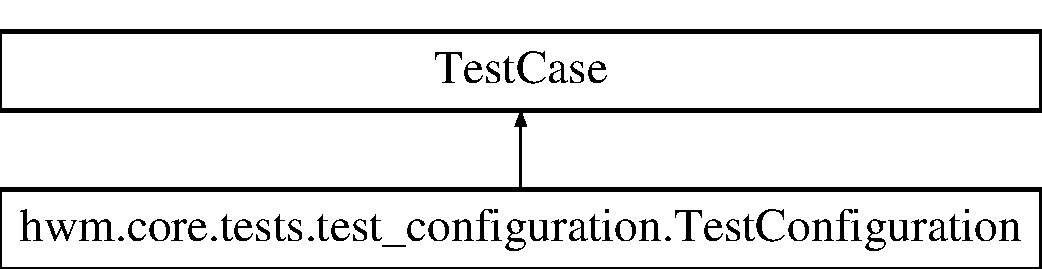
\includegraphics[height=2.000000cm]{classhwm_1_1core_1_1tests_1_1test__configuration_1_1_test_configuration}
\end{center}
\end{figure}
\subsection*{Public Member Functions}
\begin{DoxyCompactItemize}
\item 
\hypertarget{classhwm_1_1core_1_1tests_1_1test__configuration_1_1_test_configuration_a647bf2029dc0d183573c89c58d6f4096}{def {\bfseries set\-Up}}\label{classhwm_1_1core_1_1tests_1_1test__configuration_1_1_test_configuration_a647bf2029dc0d183573c89c58d6f4096}

\item 
\hypertarget{classhwm_1_1core_1_1tests_1_1test__configuration_1_1_test_configuration_a21d352adb004a3458af5667d48d90626}{def {\bfseries tear\-Down}}\label{classhwm_1_1core_1_1tests_1_1test__configuration_1_1_test_configuration_a21d352adb004a3458af5667d48d90626}

\item 
\hypertarget{classhwm_1_1core_1_1tests_1_1test__configuration_1_1_test_configuration_a84dddfc4a1966d5ededf5532d9e3c71b}{def {\bfseries test\-\_\-configuration\-\_\-setup}}\label{classhwm_1_1core_1_1tests_1_1test__configuration_1_1_test_configuration_a84dddfc4a1966d5ededf5532d9e3c71b}

\item 
\hypertarget{classhwm_1_1core_1_1tests_1_1test__configuration_1_1_test_configuration_ab2196b8bdc35a55296679b3bd121090b}{def {\bfseries test\-\_\-user\-\_\-option\-\_\-standard\-\_\-operation}}\label{classhwm_1_1core_1_1tests_1_1test__configuration_1_1_test_configuration_ab2196b8bdc35a55296679b3bd121090b}

\item 
\hypertarget{classhwm_1_1core_1_1tests_1_1test__configuration_1_1_test_configuration_a1bf684666f466141eecdc94889d22c17}{def {\bfseries test\-\_\-user\-\_\-option\-\_\-override}}\label{classhwm_1_1core_1_1tests_1_1test__configuration_1_1_test_configuration_a1bf684666f466141eecdc94889d22c17}

\item 
\hypertarget{classhwm_1_1core_1_1tests_1_1test__configuration_1_1_test_configuration_aaee6f1eaf24d095ae1413b92054e7220}{def {\bfseries test\-\_\-user\-\_\-option\-\_\-read\-\_\-nonexistent}}\label{classhwm_1_1core_1_1tests_1_1test__configuration_1_1_test_configuration_aaee6f1eaf24d095ae1413b92054e7220}

\item 
\hypertarget{classhwm_1_1core_1_1tests_1_1test__configuration_1_1_test_configuration_ae1c4d819e898334a90a72a6c53dd0951}{def {\bfseries test\-\_\-user\-\_\-option\-\_\-delete\-\_\-nonexistent}}\label{classhwm_1_1core_1_1tests_1_1test__configuration_1_1_test_configuration_ae1c4d819e898334a90a72a6c53dd0951}

\item 
\hypertarget{classhwm_1_1core_1_1tests_1_1test__configuration_1_1_test_configuration_a7ba6c7f4ece88a8adf0d268b2506caa0}{def {\bfseries test\-\_\-config\-\_\-file\-\_\-load}}\label{classhwm_1_1core_1_1tests_1_1test__configuration_1_1_test_configuration_a7ba6c7f4ece88a8adf0d268b2506caa0}

\item 
\hypertarget{classhwm_1_1core_1_1tests_1_1test__configuration_1_1_test_configuration_a1d5f214ee4f434d144f0695ab1ad0205}{def {\bfseries test\-\_\-config\-\_\-file\-\_\-invalid\-\_\-load}}\label{classhwm_1_1core_1_1tests_1_1test__configuration_1_1_test_configuration_a1d5f214ee4f434d144f0695ab1ad0205}

\item 
\hypertarget{classhwm_1_1core_1_1tests_1_1test__configuration_1_1_test_configuration_a668bcea24e6152d35e9132afdc5dd737}{def {\bfseries test\-\_\-default\-\_\-option\-\_\-set}}\label{classhwm_1_1core_1_1tests_1_1test__configuration_1_1_test_configuration_a668bcea24e6152d35e9132afdc5dd737}

\item 
\hypertarget{classhwm_1_1core_1_1tests_1_1test__configuration_1_1_test_configuration_a14cfcee6ef411abba643eb4a7fc617f2}{def {\bfseries test\-\_\-default\-\_\-option\-\_\-override}}\label{classhwm_1_1core_1_1tests_1_1test__configuration_1_1_test_configuration_a14cfcee6ef411abba643eb4a7fc617f2}

\item 
\hypertarget{classhwm_1_1core_1_1tests_1_1test__configuration_1_1_test_configuration_adcda0a611a1d0ce2957bfd3672366628}{def {\bfseries test\-\_\-required\-\_\-option\-\_\-not\-\_\-set}}\label{classhwm_1_1core_1_1tests_1_1test__configuration_1_1_test_configuration_adcda0a611a1d0ce2957bfd3672366628}

\item 
\hypertarget{classhwm_1_1core_1_1tests_1_1test__configuration_1_1_test_configuration_a696ce64435e758aee6434a729d1d08c5}{def {\bfseries test\-\_\-protected\-\_\-option\-\_\-read}}\label{classhwm_1_1core_1_1tests_1_1test__configuration_1_1_test_configuration_a696ce64435e758aee6434a729d1d08c5}

\item 
\hypertarget{classhwm_1_1core_1_1tests_1_1test__configuration_1_1_test_configuration_a5900af776af16be95fe427880cdf78ef}{def {\bfseries test\-\_\-protected\-\_\-option\-\_\-set\-\_\-protection}}\label{classhwm_1_1core_1_1tests_1_1test__configuration_1_1_test_configuration_a5900af776af16be95fe427880cdf78ef}

\item 
\hypertarget{classhwm_1_1core_1_1tests_1_1test__configuration_1_1_test_configuration_afff950a936cd73d1542e8b16398041b6}{def {\bfseries test\-\_\-protected\-\_\-option\-\_\-delete\-\_\-protection}}\label{classhwm_1_1core_1_1tests_1_1test__configuration_1_1_test_configuration_afff950a936cd73d1542e8b16398041b6}

\end{DoxyCompactItemize}
\subsection*{Public Attributes}
\begin{DoxyCompactItemize}
\item 
\hypertarget{classhwm_1_1core_1_1tests_1_1test__configuration_1_1_test_configuration_a7b03d30cc9acb5deeb12a55d1cdea015}{{\bfseries config}}\label{classhwm_1_1core_1_1tests_1_1test__configuration_1_1_test_configuration_a7b03d30cc9acb5deeb12a55d1cdea015}

\item 
\hypertarget{classhwm_1_1core_1_1tests_1_1test__configuration_1_1_test_configuration_af45c587122dd349022c2730e6205906d}{{\bfseries source\-\_\-data\-\_\-directory}}\label{classhwm_1_1core_1_1tests_1_1test__configuration_1_1_test_configuration_af45c587122dd349022c2730e6205906d}

\end{DoxyCompactItemize}


\subsection{Detailed Description}
This test case tests the functionality of the configuration module (and Config class). 

\begin{DoxyNote}{Note}
The configuration module creates a singleton instance of the Config class (accessed with Configuration). 
\end{DoxyNote}


The documentation for this class was generated from the following file\-:\begin{DoxyCompactItemize}
\item 
C\-:/\-Users/\-Jimmy/\-Documents/\-Files/\-Work/\-Active Projects/\-M\-X\-L/mercury2/\-Hardware\-\_\-\-Manager/hwm/core/tests/test\-\_\-configuration.\-py\end{DoxyCompactItemize}

\hypertarget{classhwm_1_1sessions_1_1tests_1_1test__coordinator_1_1_test_coordinator}{\section{hwm.\-sessions.\-tests.\-test\-\_\-coordinator.\-Test\-Coordinator Class Reference}
\label{classhwm_1_1sessions_1_1tests_1_1test__coordinator_1_1_test_coordinator}\index{hwm.\-sessions.\-tests.\-test\-\_\-coordinator.\-Test\-Coordinator@{hwm.\-sessions.\-tests.\-test\-\_\-coordinator.\-Test\-Coordinator}}
}


This test suite tests the functionality of the session coordinator.  


Inheritance diagram for hwm.\-sessions.\-tests.\-test\-\_\-coordinator.\-Test\-Coordinator\-:\begin{figure}[H]
\begin{center}
\leavevmode
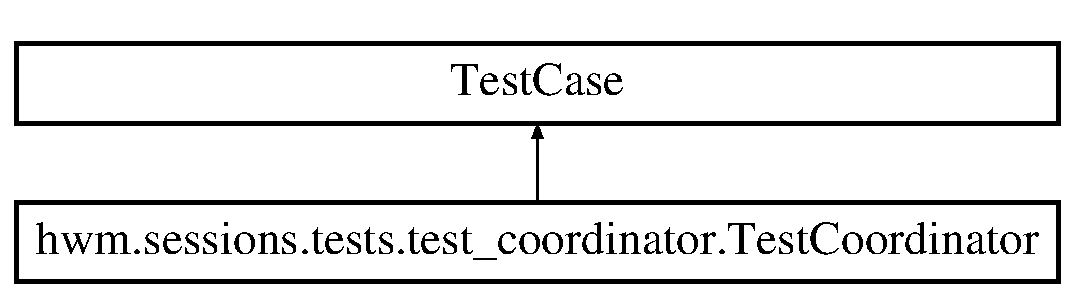
\includegraphics[height=2.000000cm]{classhwm_1_1sessions_1_1tests_1_1test__coordinator_1_1_test_coordinator}
\end{center}
\end{figure}
\subsection*{Public Member Functions}
\begin{DoxyCompactItemize}
\item 
\hypertarget{classhwm_1_1sessions_1_1tests_1_1test__coordinator_1_1_test_coordinator_ad515ad14dc1a984de607635a81a67455}{def {\bfseries set\-Up}}\label{classhwm_1_1sessions_1_1tests_1_1test__coordinator_1_1_test_coordinator_ad515ad14dc1a984de607635a81a67455}

\item 
\hypertarget{classhwm_1_1sessions_1_1tests_1_1test__coordinator_1_1_test_coordinator_a363d58d2e8912298a07f77b7990e039a}{def {\bfseries tear\-Down}}\label{classhwm_1_1sessions_1_1tests_1_1test__coordinator_1_1_test_coordinator_a363d58d2e8912298a07f77b7990e039a}

\item 
\hypertarget{classhwm_1_1sessions_1_1tests_1_1test__coordinator_1_1_test_coordinator_a3327bf6cf9f23d00fe71d525f409b82f}{def \hyperlink{classhwm_1_1sessions_1_1tests_1_1test__coordinator_1_1_test_coordinator_a3327bf6cf9f23d00fe71d525f409b82f}{test\-\_\-schedule\-\_\-update}}\label{classhwm_1_1sessions_1_1tests_1_1test__coordinator_1_1_test_coordinator_a3327bf6cf9f23d00fe71d525f409b82f}

\begin{DoxyCompactList}\small\item\em This test checks that the session coordinator can correctly instruct the schedule manager to update its schedule. \end{DoxyCompactList}\item 
\hypertarget{classhwm_1_1sessions_1_1tests_1_1test__coordinator_1_1_test_coordinator_a1dcc013c1674fd593b0f2bb86f7ec325}{def \hyperlink{classhwm_1_1sessions_1_1tests_1_1test__coordinator_1_1_test_coordinator_a1dcc013c1674fd593b0f2bb86f7ec325}{test\-\_\-active\-\_\-reservation\-\_\-session\-\_\-creation}}\label{classhwm_1_1sessions_1_1tests_1_1test__coordinator_1_1_test_coordinator_a1dcc013c1674fd593b0f2bb86f7ec325}

\begin{DoxyCompactList}\small\item\em This test verifies that the session coordinator can correctly create (and skip) usage sessions from the reservation schedule. \end{DoxyCompactList}\end{DoxyCompactItemize}
\subsection*{Public Attributes}
\begin{DoxyCompactItemize}
\item 
\hypertarget{classhwm_1_1sessions_1_1tests_1_1test__coordinator_1_1_test_coordinator_a3f7b40a4155ad7addb3dff58a7bf736a}{{\bfseries config}}\label{classhwm_1_1sessions_1_1tests_1_1test__coordinator_1_1_test_coordinator_a3f7b40a4155ad7addb3dff58a7bf736a}

\item 
\hypertarget{classhwm_1_1sessions_1_1tests_1_1test__coordinator_1_1_test_coordinator_a0967f2e46b04d37f832d79e45121ca29}{{\bfseries source\-\_\-data\-\_\-directory}}\label{classhwm_1_1sessions_1_1tests_1_1test__coordinator_1_1_test_coordinator_a0967f2e46b04d37f832d79e45121ca29}

\end{DoxyCompactItemize}


\subsection{Detailed Description}
This test suite tests the functionality of the session coordinator. 

The documentation for this class was generated from the following file\-:\begin{DoxyCompactItemize}
\item 
C\-:/\-Users/\-Jimmy/\-Documents/\-Files/\-Work/\-Active Projects/\-M\-X\-L/mercury2/\-Hardware\-\_\-\-Manager/hwm/sessions/tests/test\-\_\-coordinator.\-py\end{DoxyCompactItemize}

\hypertarget{classhwm_1_1hardware_1_1pipelines_1_1tests_1_1test__pipeline__manager_1_1_test_pipeline_manager}{\section{hwm.\-hardware.\-pipelines.\-tests.\-test\-\_\-pipeline\-\_\-manager.\-Test\-Pipeline\-Manager Class Reference}
\label{classhwm_1_1hardware_1_1pipelines_1_1tests_1_1test__pipeline__manager_1_1_test_pipeline_manager}\index{hwm.\-hardware.\-pipelines.\-tests.\-test\-\_\-pipeline\-\_\-manager.\-Test\-Pipeline\-Manager@{hwm.\-hardware.\-pipelines.\-tests.\-test\-\_\-pipeline\-\_\-manager.\-Test\-Pipeline\-Manager}}
}


This collection of tests tests the hardware pipeline manager, which is responsible for managing access to the individual hardware pipelines.  


Inheritance diagram for hwm.\-hardware.\-pipelines.\-tests.\-test\-\_\-pipeline\-\_\-manager.\-Test\-Pipeline\-Manager\-:\begin{figure}[H]
\begin{center}
\leavevmode
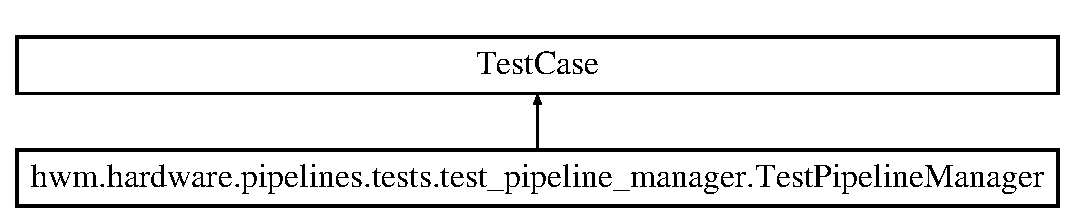
\includegraphics[height=2.000000cm]{classhwm_1_1hardware_1_1pipelines_1_1tests_1_1test__pipeline__manager_1_1_test_pipeline_manager}
\end{center}
\end{figure}
\subsection*{Public Member Functions}
\begin{DoxyCompactItemize}
\item 
\hypertarget{classhwm_1_1hardware_1_1pipelines_1_1tests_1_1test__pipeline__manager_1_1_test_pipeline_manager_ac179d43830017f0a99bf9712f7cbee81}{def {\bfseries set\-Up}}\label{classhwm_1_1hardware_1_1pipelines_1_1tests_1_1test__pipeline__manager_1_1_test_pipeline_manager_ac179d43830017f0a99bf9712f7cbee81}

\item 
\hypertarget{classhwm_1_1hardware_1_1pipelines_1_1tests_1_1test__pipeline__manager_1_1_test_pipeline_manager_a72737439c025f32b64a8d67987736046}{def {\bfseries tear\-Down}}\label{classhwm_1_1hardware_1_1pipelines_1_1tests_1_1test__pipeline__manager_1_1_test_pipeline_manager_a72737439c025f32b64a8d67987736046}

\item 
\hypertarget{classhwm_1_1hardware_1_1pipelines_1_1tests_1_1test__pipeline__manager_1_1_test_pipeline_manager_a7b4162cdcb61eaf8e7991d13b2432897}{def \hyperlink{classhwm_1_1hardware_1_1pipelines_1_1tests_1_1test__pipeline__manager_1_1_test_pipeline_manager_a7b4162cdcb61eaf8e7991d13b2432897}{test\-\_\-initialization\-\_\-errors}}\label{classhwm_1_1hardware_1_1pipelines_1_1tests_1_1test__pipeline__manager_1_1_test_pipeline_manager_a7b4162cdcb61eaf8e7991d13b2432897}

\begin{DoxyCompactList}\small\item\em Verifies that the pipeline manager raises exceptions as appropriate during initialization. \end{DoxyCompactList}\item 
def \hyperlink{classhwm_1_1hardware_1_1pipelines_1_1tests_1_1test__pipeline__manager_1_1_test_pipeline_manager_a1f51d3e12b2c7028d2bb7eaf8fc30024}{test\-\_\-pipeline\-\_\-invalid\-\_\-config}
\begin{DoxyCompactList}\small\item\em Tests that the pipeline manager correctly rejects some invalid pipeline configurations (as validated by Pipeline.\-\_\-setup\-\_\-pipeline()). \end{DoxyCompactList}\item 
\hypertarget{classhwm_1_1hardware_1_1pipelines_1_1tests_1_1test__pipeline__manager_1_1_test_pipeline_manager_afc95e79fcb438a9a1bbbc1987632db6c}{def \hyperlink{classhwm_1_1hardware_1_1pipelines_1_1tests_1_1test__pipeline__manager_1_1_test_pipeline_manager_afc95e79fcb438a9a1bbbc1987632db6c}{test\-\_\-pipeline\-\_\-get}}\label{classhwm_1_1hardware_1_1pipelines_1_1tests_1_1test__pipeline__manager_1_1_test_pipeline_manager_afc95e79fcb438a9a1bbbc1987632db6c}

\begin{DoxyCompactList}\small\item\em Tests that the pipeline manager can correctly return a specified pipeline. \end{DoxyCompactList}\end{DoxyCompactItemize}
\subsection*{Public Attributes}
\begin{DoxyCompactItemize}
\item 
\hypertarget{classhwm_1_1hardware_1_1pipelines_1_1tests_1_1test__pipeline__manager_1_1_test_pipeline_manager_ad92a77f755c8cebb0389690a65cb1f93}{{\bfseries config}}\label{classhwm_1_1hardware_1_1pipelines_1_1tests_1_1test__pipeline__manager_1_1_test_pipeline_manager_ad92a77f755c8cebb0389690a65cb1f93}

\item 
\hypertarget{classhwm_1_1hardware_1_1pipelines_1_1tests_1_1test__pipeline__manager_1_1_test_pipeline_manager_afd711b88d77f50caea5c8503435451fd}{{\bfseries source\-\_\-data\-\_\-directory}}\label{classhwm_1_1hardware_1_1pipelines_1_1tests_1_1test__pipeline__manager_1_1_test_pipeline_manager_afd711b88d77f50caea5c8503435451fd}

\item 
\hypertarget{classhwm_1_1hardware_1_1pipelines_1_1tests_1_1test__pipeline__manager_1_1_test_pipeline_manager_aaee9fbc81e51d86d01d58504e59f02ef}{{\bfseries command\-\_\-parser}}\label{classhwm_1_1hardware_1_1pipelines_1_1tests_1_1test__pipeline__manager_1_1_test_pipeline_manager_aaee9fbc81e51d86d01d58504e59f02ef}

\item 
\hypertarget{classhwm_1_1hardware_1_1pipelines_1_1tests_1_1test__pipeline__manager_1_1_test_pipeline_manager_aed029f977f1d05573bf75371a4c9c4fc}{{\bfseries session\-\_\-coordinator}}\label{classhwm_1_1hardware_1_1pipelines_1_1tests_1_1test__pipeline__manager_1_1_test_pipeline_manager_aed029f977f1d05573bf75371a4c9c4fc}

\item 
\hypertarget{classhwm_1_1hardware_1_1pipelines_1_1tests_1_1test__pipeline__manager_1_1_test_pipeline_manager_a70f550b1ebf4f5e2eacaedc73db067e0}{{\bfseries device\-\_\-manager}}\label{classhwm_1_1hardware_1_1pipelines_1_1tests_1_1test__pipeline__manager_1_1_test_pipeline_manager_a70f550b1ebf4f5e2eacaedc73db067e0}

\end{DoxyCompactItemize}
\subsection*{Private Member Functions}
\begin{DoxyCompactItemize}
\item 
def \hyperlink{classhwm_1_1hardware_1_1pipelines_1_1tests_1_1test__pipeline__manager_1_1_test_pipeline_manager_a4c08b28c93be6c3debcd8aaddb2de5e2}{\-\_\-reset\-\_\-device\-\_\-manager}
\begin{DoxyCompactList}\small\item\em Resets the device manager instance. \end{DoxyCompactList}\item 
\hypertarget{classhwm_1_1hardware_1_1pipelines_1_1tests_1_1test__pipeline__manager_1_1_test_pipeline_manager_a78d66e796179f40f732ce7d1d76b76b5}{def {\bfseries \-\_\-reset\-\_\-config\-\_\-entries}}\label{classhwm_1_1hardware_1_1pipelines_1_1tests_1_1test__pipeline__manager_1_1_test_pipeline_manager_a78d66e796179f40f732ce7d1d76b76b5}

\end{DoxyCompactItemize}


\subsection{Detailed Description}
This collection of tests tests the hardware pipeline manager, which is responsible for managing access to the individual hardware pipelines. 

\subsection{Member Function Documentation}
\hypertarget{classhwm_1_1hardware_1_1pipelines_1_1tests_1_1test__pipeline__manager_1_1_test_pipeline_manager_a4c08b28c93be6c3debcd8aaddb2de5e2}{\index{hwm\-::hardware\-::pipelines\-::tests\-::test\-\_\-pipeline\-\_\-manager\-::\-Test\-Pipeline\-Manager@{hwm\-::hardware\-::pipelines\-::tests\-::test\-\_\-pipeline\-\_\-manager\-::\-Test\-Pipeline\-Manager}!\-\_\-reset\-\_\-device\-\_\-manager@{\-\_\-reset\-\_\-device\-\_\-manager}}
\index{\-\_\-reset\-\_\-device\-\_\-manager@{\-\_\-reset\-\_\-device\-\_\-manager}!hwm::hardware::pipelines::tests::test_pipeline_manager::TestPipelineManager@{hwm\-::hardware\-::pipelines\-::tests\-::test\-\_\-pipeline\-\_\-manager\-::\-Test\-Pipeline\-Manager}}
\subsubsection[{\-\_\-reset\-\_\-device\-\_\-manager}]{\setlength{\rightskip}{0pt plus 5cm}def hwm.\-hardware.\-pipelines.\-tests.\-test\-\_\-pipeline\-\_\-manager.\-Test\-Pipeline\-Manager.\-\_\-reset\-\_\-device\-\_\-manager (
\begin{DoxyParamCaption}
\item[{}]{self, }
\item[{}]{command\-\_\-parser}
\end{DoxyParamCaption}
)\hspace{0.3cm}{\ttfamily [private]}}}\label{classhwm_1_1hardware_1_1pipelines_1_1tests_1_1test__pipeline__manager_1_1_test_pipeline_manager_a4c08b28c93be6c3debcd8aaddb2de5e2}


Resets the device manager instance. 

This is required if multiple pipeline configurations are tested in the same test method because the device pipeline registrations don't get reset when the pipeline manager does.


\begin{DoxyParams}{Parameters}
{\em command\-\_\-parser} & The active Command\-Parser instance. \\
\hline
\end{DoxyParams}
\hypertarget{classhwm_1_1hardware_1_1pipelines_1_1tests_1_1test__pipeline__manager_1_1_test_pipeline_manager_a1f51d3e12b2c7028d2bb7eaf8fc30024}{\index{hwm\-::hardware\-::pipelines\-::tests\-::test\-\_\-pipeline\-\_\-manager\-::\-Test\-Pipeline\-Manager@{hwm\-::hardware\-::pipelines\-::tests\-::test\-\_\-pipeline\-\_\-manager\-::\-Test\-Pipeline\-Manager}!test\-\_\-pipeline\-\_\-invalid\-\_\-config@{test\-\_\-pipeline\-\_\-invalid\-\_\-config}}
\index{test\-\_\-pipeline\-\_\-invalid\-\_\-config@{test\-\_\-pipeline\-\_\-invalid\-\_\-config}!hwm::hardware::pipelines::tests::test_pipeline_manager::TestPipelineManager@{hwm\-::hardware\-::pipelines\-::tests\-::test\-\_\-pipeline\-\_\-manager\-::\-Test\-Pipeline\-Manager}}
\subsubsection[{test\-\_\-pipeline\-\_\-invalid\-\_\-config}]{\setlength{\rightskip}{0pt plus 5cm}def hwm.\-hardware.\-pipelines.\-tests.\-test\-\_\-pipeline\-\_\-manager.\-Test\-Pipeline\-Manager.\-test\-\_\-pipeline\-\_\-invalid\-\_\-config (
\begin{DoxyParamCaption}
\item[{}]{self}
\end{DoxyParamCaption}
)}}\label{classhwm_1_1hardware_1_1pipelines_1_1tests_1_1test__pipeline__manager_1_1_test_pipeline_manager_a1f51d3e12b2c7028d2bb7eaf8fc30024}


Tests that the pipeline manager correctly rejects some invalid pipeline configurations (as validated by Pipeline.\-\_\-setup\-\_\-pipeline()). 

This is also tested directly by the Pipeline unit test suite. 

The documentation for this class was generated from the following file\-:\begin{DoxyCompactItemize}
\item 
hwm/hardware/pipelines/tests/test\-\_\-pipeline\-\_\-manager.\-py\end{DoxyCompactItemize}

\hypertarget{classhwm_1_1sessions_1_1tests_1_1test__schedule_1_1_test_schedule}{\section{hwm.\-sessions.\-tests.\-test\-\_\-schedule.\-Test\-Schedule Class Reference}
\label{classhwm_1_1sessions_1_1tests_1_1test__schedule_1_1_test_schedule}\index{hwm.\-sessions.\-tests.\-test\-\_\-schedule.\-Test\-Schedule@{hwm.\-sessions.\-tests.\-test\-\_\-schedule.\-Test\-Schedule}}
}


This test suite tests the functionality of the schedule manager (Schedule\-Manager).  


Inheritance diagram for hwm.\-sessions.\-tests.\-test\-\_\-schedule.\-Test\-Schedule\-:\begin{figure}[H]
\begin{center}
\leavevmode
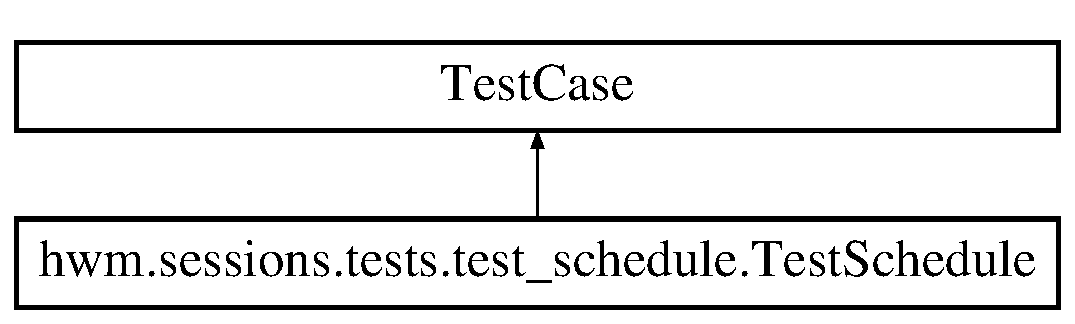
\includegraphics[height=2.000000cm]{classhwm_1_1sessions_1_1tests_1_1test__schedule_1_1_test_schedule}
\end{center}
\end{figure}
\subsection*{Public Member Functions}
\begin{DoxyCompactItemize}
\item 
\hypertarget{classhwm_1_1sessions_1_1tests_1_1test__schedule_1_1_test_schedule_a53c04d1ce7982c94c18e193f5fae6de3}{def {\bfseries set\-Up}}\label{classhwm_1_1sessions_1_1tests_1_1test__schedule_1_1_test_schedule_a53c04d1ce7982c94c18e193f5fae6de3}

\item 
\hypertarget{classhwm_1_1sessions_1_1tests_1_1test__schedule_1_1_test_schedule_a81669427da2aaa2ff48f0d21c8925ee2}{def \hyperlink{classhwm_1_1sessions_1_1tests_1_1test__schedule_1_1_test_schedule_a81669427da2aaa2ff48f0d21c8925ee2}{test\-\_\-local\-\_\-file\-\_\-load}}\label{classhwm_1_1sessions_1_1tests_1_1test__schedule_1_1_test_schedule_a81669427da2aaa2ff48f0d21c8925ee2}

\begin{DoxyCompactList}\small\item\em Tests the ability of the Schedule manager to download a valid dummy schedule from the local disk and update its local schedule copy. \end{DoxyCompactList}\item 
\hypertarget{classhwm_1_1sessions_1_1tests_1_1test__schedule_1_1_test_schedule_ae11c8a73b939a92ff398b948b0afa015}{def \hyperlink{classhwm_1_1sessions_1_1tests_1_1test__schedule_1_1_test_schedule_ae11c8a73b939a92ff398b948b0afa015}{test\-\_\-local\-\_\-file\-\_\-load\-\_\-invalid\-\_\-schema}}\label{classhwm_1_1sessions_1_1tests_1_1test__schedule_1_1_test_schedule_ae11c8a73b939a92ff398b948b0afa015}

\begin{DoxyCompactList}\small\item\em Verifies that Schedule\-Manager rejects schedules that don't fit the schedule schema requirements (see included documentation for requirements). \end{DoxyCompactList}\item 
\hypertarget{classhwm_1_1sessions_1_1tests_1_1test__schedule_1_1_test_schedule_ae9a9f2dd3dbd2169a24bfc6210f5b238}{def \hyperlink{classhwm_1_1sessions_1_1tests_1_1test__schedule_1_1_test_schedule_ae9a9f2dd3dbd2169a24bfc6210f5b238}{test\-\_\-local\-\_\-file\-\_\-load\-\_\-missing}}\label{classhwm_1_1sessions_1_1tests_1_1test__schedule_1_1_test_schedule_ae9a9f2dd3dbd2169a24bfc6210f5b238}

\begin{DoxyCompactList}\small\item\em Tests that the Schedule\-Manager returns an error if a missing schedule file is requested. \end{DoxyCompactList}\item 
\hypertarget{classhwm_1_1sessions_1_1tests_1_1test__schedule_1_1_test_schedule_aad883af594f5058a04fb1b6bc2dd5d9a}{def \hyperlink{classhwm_1_1sessions_1_1tests_1_1test__schedule_1_1_test_schedule_aad883af594f5058a04fb1b6bc2dd5d9a}{test\-\_\-remote\-\_\-file\-\_\-load\-\_\-missing}}\label{classhwm_1_1sessions_1_1tests_1_1test__schedule_1_1_test_schedule_aad883af594f5058a04fb1b6bc2dd5d9a}

\begin{DoxyCompactList}\small\item\em Tests the schedule manager's ability to respond to an invalid schedule U\-R\-L. \end{DoxyCompactList}\item 
def \hyperlink{classhwm_1_1sessions_1_1tests_1_1test__schedule_1_1_test_schedule_ab2481441aa193770ce6812e1728e4b77}{test\-\_\-get\-\_\-active\-\_\-reservations}
\begin{DoxyCompactList}\small\item\em Tests that the schedule manager returns the reservations that are active (i.\-e. \end{DoxyCompactList}\end{DoxyCompactItemize}
\subsection*{Public Attributes}
\begin{DoxyCompactItemize}
\item 
\hypertarget{classhwm_1_1sessions_1_1tests_1_1test__schedule_1_1_test_schedule_a6d48e1aaf3b1e1267e8a69b1e23b104b}{{\bfseries source\-\_\-data\-\_\-directory}}\label{classhwm_1_1sessions_1_1tests_1_1test__schedule_1_1_test_schedule_a6d48e1aaf3b1e1267e8a69b1e23b104b}

\end{DoxyCompactItemize}


\subsection{Detailed Description}
This test suite tests the functionality of the schedule manager (Schedule\-Manager). 

\subsection{Member Function Documentation}
\hypertarget{classhwm_1_1sessions_1_1tests_1_1test__schedule_1_1_test_schedule_ab2481441aa193770ce6812e1728e4b77}{\index{hwm\-::sessions\-::tests\-::test\-\_\-schedule\-::\-Test\-Schedule@{hwm\-::sessions\-::tests\-::test\-\_\-schedule\-::\-Test\-Schedule}!test\-\_\-get\-\_\-active\-\_\-reservations@{test\-\_\-get\-\_\-active\-\_\-reservations}}
\index{test\-\_\-get\-\_\-active\-\_\-reservations@{test\-\_\-get\-\_\-active\-\_\-reservations}!hwm::sessions::tests::test_schedule::TestSchedule@{hwm\-::sessions\-::tests\-::test\-\_\-schedule\-::\-Test\-Schedule}}
\subsubsection[{test\-\_\-get\-\_\-active\-\_\-reservations}]{\setlength{\rightskip}{0pt plus 5cm}def hwm.\-sessions.\-tests.\-test\-\_\-schedule.\-Test\-Schedule.\-test\-\_\-get\-\_\-active\-\_\-reservations (
\begin{DoxyParamCaption}
\item[{}]{self}
\end{DoxyParamCaption}
)}}\label{classhwm_1_1sessions_1_1tests_1_1test__schedule_1_1_test_schedule_ab2481441aa193770ce6812e1728e4b77}


Tests that the schedule manager returns the reservations that are active (i.\-e. 

time\-\_\-start $<$ current time $<$ time\-\_\-end), while ignoring the inactive ones.

\begin{DoxyNote}{Note}
The end time of one of the reservations in the test schedule is set to 2019 to make this test pass. 
\end{DoxyNote}


The documentation for this class was generated from the following file\-:\begin{DoxyCompactItemize}
\item 
hwm/sessions/tests/test\-\_\-schedule.\-py\end{DoxyCompactItemize}

\addcontentsline{toc}{part}{Index}
\printindex
\end{document}
